% !TEX TS-program = XeLaTeX
%
% Περάστε στο πακέτο cseuoi-thesis τις κατάλληλες επιλογές για τη διατριβή σας
%
%\documentclass[gr,phd]{cseuoi-thesis} % Διδακτορικό (στα Ελληνικά)
\documentclass[en,msc,systems]{cseuoi-thesis} % Μεταπτυχιακό με εξειδίκευση στα Υπολογιστικά Συστήματα (στα Αγγλικά)
%\documentclass[en,msc,theory]{cseuoi-thesis} % Μεταπτυχιακό με εξειδίκευση στη Θεωρία Επιστήμης Υπολογιστών (στα Αγγλικά)
%\documentclass[en,msc,software]{cseuoi-thesis} % Μεταπτυχαικό με εξειδίκευση στο Λογισμικό (στα Αγγλικά)
%\documentclass[en,msc,scicomp]{cseuoi-thesis} % Μεταπτυχιακό με εξειδίκευση στους Επιστημονικούς Υπολογισμούς (στα Αγγλικά)
%\documentclass[en,msc,techapps]{cseuoi-thesis} % Μεταπτυχιακό με εξειδίκευση στις Τεχνολογίες - Εφαρμογές (στα Αγγλικά)


% 
% Συμπληρώστε τα στοιχεία σας στις παρακάτω εντολές (αφαιρώντας το \colorbox{gray}{})
%
\titleEn{Reducing Polarization in Social Media}
\authorEn{Leonidas Boutsikaris}
\arthro{τον}
\aitiatiki{}
\dateEn{April 2020}
\advisorEn{Panayiotis Tsaparas, Assistant Professor}



% 
% Εξεταστική επιτροπή για ΜΔΕ
%
\MSCexaminer{Panayiotis Tsaparas}{Associate Professor}%
    {Department of Computer Science and Engineering, University of Ioannina (Supervisor)}
\MSCexaminer{? ?}{Associate Professor}%
    {Department of Computer Science and Engineering, University of Ioannina }
\MSCexaminer{? ?}{Associate Professor}%
    {Department of Computer Science and Engineering, University of Ioannina }


% Πακέτο για την εμφάνιση περιθωρίων (χρήσιμο για την εύρεση overfull boxes)
%\usepackage{showframe}

% Πακέτο για τη διατήρηση των floats (εικόνες κ.α.) εντός των ενοτήτων
%\usepackage[section]{placeins}



\begin{document}

% Σελίδες χωρίς αρίθμηση
\pagenumbering{gobble}

% Εκτύπωση της σελίδας τίτλου
\maketitle

% Εκτύπωση της σελίδας με τις επιτροπές
\makecommittees

% Αρχικοποίηση του minitoc
\dominitoc[n]

%\chapter*{\cseafierwsi}

Η σελίδα αυτή είναι προαιρετική και περιέχει αφιέρωση σε κάποιο σημαντικό πρόσωπο.

\bigskip

\noindent Προτεινόμενο: 1-2 γραμμές.

\noindent Μέγιστο: 1 σελίδα.
 % Προαιρετικό
%\chapter*{\cseeuxaristies}

Η σελίδα αυτή είναι προαιρετική και περιέχει ευχαριστίες σε άτομα που βοήθησαν με οποιονδήποτε τρόπο τον συγγραφέα της διατριβής.

\bigskip

\noindent Προτεινόμενο: 10-15 γραμμές.

\noindent Μέγιστο: 1 σελίδα. % Προαιρετικό


% Σελίδες με αρίθμηση i, ii, iii, iv, ...
\pagenumbering{roman}

% Περιεχόμενα
\pdfbookmark{\contentsname}{contents} % hyperref
\tableofcontents

% Κατάλογος Σχημάτων
%\addstarredchapterc{\listfigurename} % minitoc
%\listoffigures

% Κατάλογος Πινάκων
%\addstarredchapterc{\listtablename} % minitoc
%\listoftables

% Κατάλογος Αλγορίθμων
%\addstarredchapterc{\listalgorithmname} % minitoc
%\listof{algorithm}{\listalgorithmname}

%\chapter*{\glossaryname}
% Εισαγωγή του κεφάλαιου στα περιεχόμενα
\addstarredchapter{\glossaryname} %minitoc

Η σελίδα αυτή είναι προαιρετική.
Περιέχει ορισμούς και επεξηγήσεις εννοιών, όρων, συντομεύσεων, και συμβολισμών.
Αν η έκτασή τους είναι μεγαλύτερη από δύο σελίδες τότε πρέπει να πάει στο τέλος της διατριβής, αμέσως μετά τα παραρτήματα. % Προαιρετικό

% Περίληψη και εκτεταμένη περίληψη
%\chapter*{\abstractname}
\addstarredchapter{\abstractname} % minitoc

\noindent We know for a fact that opinions are formed through social interactions. Online communities offer public access to social disputes on controversial matters that allow the study and moderation of them. The majority of studies in social networks are based on the Friedkin-Johnsen model.
\\
\\
Users of online communities are receiving biased information that amplify their own viewpoints. This creates a fragmented community and users interact only with individuals that hold the same opinions. In this thesis we use the polarization index to measure the polarization of a social graph.
\\
\\We try to reduce the polarization by connecting individuals. We propose new social connections between different and extreme opinions by following the intuition of the Friedkin-Johnsen model. 
\\
\\
Finally, probabilities are adopted to our heuristic algorithms that now make selections based on how probable is the acceptance of a recommendation of a new social connection. 

\bigskip

%\chapter*{\cseextabstract}
\addstarredchapter{\cseextabstract} % minitoc

%\makecseextabstract


\noindent Εκτεταμένη περίληψη της εργασίας στην αντίθετη γλώσσα από αυτήν του κειμένου.
Αν το κείμενο είναι στα Ελληνικά τότε αυτή η σελίδα πρέπει να είναι στα Αγγλικά.
Αν το κείμενο είναι στα Αγγλικά τότε αυτή η σελίδα πρέπει να είναι στα Ελληνικά.

\bigskip

\noindent Προτεινόμενο: 2 σελίδες.

\noindent Μέγιστο: 4 σελίδες.


% Σελίδες με αρίθμηση 1, 2, 3, 4, ...
\pagenumbering{arabic}


% Εισαγωγή των κεφαλαίων
\chapter{Introduction and the Theory Behind Polarization}
\label{ch:Introduction}


\section{Introduction}
\label{sec:Objectives}

Polarization describes the division of people into two contrasting groups or sets of opinions or beliefs. The term is used in various domains such as politics and social studies. For example political polarization refers to the divergence of political attitudes to ideological extremes. Social studies use this term to  describe the segregation within a society in terms of income inequality or social and class status. Currently social media have a big role as a source of news and information and a lot of the related discussions of people have gone online. Polarization is linked with harmful effects such as intensifying stereotypes and creating echo chambers. In echo chambers individuals get their news only from like-minded people as they share and reinforce one another’s opinions. Additionally the fact that people tend to ignore opposing views in combination with algorithmic personalization results a significant increase of polarization.

\section{Social and Psychological Factors}

Individuals experience discomfort when given data that actively challenge their opinions. In the field of psychology, cognitive dissonance occurs when a person holds two or more contradictory beliefs, ideas, or values and experiences psychological stress because of that. In simple terms dissonance is defined as a the lack of agreement.
Individuals want to reduce the discomfort that is caused from cognitive dissonance. Reduction occurs by strengthening opinions that come in agreement with their own and downplaying everything that challenges them. This leads individuals to a selective exposure on information \cite{jonasHardtFreyThelen2001}. Selective exposure is also demonstrated in groups. Furthermore people assign themselves with social identities. The self-categorization theory stems from the social identity theory, which holds that conformity stems from psychological processes. Accordingly, proponents of the self-categorization model hold that group polarization occurs because individuals identify with a particular group and conform to a prototypical group position that is more extreme than the group mean. It is shown that groups of people tend to make decisions that are more extreme than the initial inclination of its members \cite{sunstein}.

\label{sec:Structure}

\section{Polarization online}

Online entities such as news or social media platforms are aware of their users opinions  and aim to maximize their satisfaction. As discussed above, platforms will present content in a way that minimizes psychological stress. This leads to media bias. Media bias is the bias or perceived bias of journalists and news producers within the mass media in the selection of many events and stories that are reported and how they are covered. When this happens online, personalization of the content creates algorithmic bias. Algorithmic bias describes systematic and repeatable errors in a computer system that create unfair outcomes, such as privileging one arbitrary group of users over others. Bias can emerge due to many factors like the design of the algorithm. Due to personalization we don't see the same content and this is the main reason for the formation of filter bubbles.

\section{Filter Bubbles}

Filter bubbles are the echo chambers of social media. In news media, an echo chamber is a metaphorical description of a situation in which beliefs  and opinions are strengthened by communication and repetition inside a closed system. It is important to distinguish the difference between echo chambers and filter bubbles. This two concepts are almost identical, however,  filter bubbles are a result of algorithms that choose content based on previous online behaviour, as with search histories or online shopping activity.



\chapter{Related Work}
\label{ch:Instructions}


\section{Measuring the Polarization of a Network}
\label{sec:Submission}

At first we have to measure the opinion polarization in a social Network. The actions and information of a user can give us insights about his opinions on a topic e.g. accounts a user follows, content they repost, comments they make , etc. Using this information we can measure the polarization. 
\\
\\
Assume a graph $G = (V,E)$ representing a network that is connected and undirected. $Z$ will be the vector of expressed opinions for the whole network. Each value $Z_i$ of the vector will represent a node and can be computed with the opinion-formation model of Friedkin and Johnsen. 
\\
\\
The length of the opinion vector $||z|| ^2$ measures  the polarization and  $\pi(z) = \frac{||z|| ^2}n$ is defined as the polarization index of the network, where  $n$ is the number of nodes in the graph so the polarization index can be independent of the network size. 
\\
\\
There is a direct link between this opinion model and random walks. Given the graph $G = (V,E)$ we can construct the augmented graph $H(V∪X, E∪R)$. For each vertex of  $V$ we will add a new vertex on $X$ and a directed edge $(v_i,x_i)$ in $R$. 
\\
\\
The node $x_i$ corresponds to the internal opinion of the node $v_i$. In the model we follow $z_j$ or else the expressed opinion of a user that can be computed by the probability of $P(x_i |v_j)$. This probability represents that a random walk on the augmented graph that started from the node $V_j$ ended at the node $X_i$ or else how much likely the probability of user $V_j$ adopting the opinion of user $V_i$. This probability depends on the structure of the graph. 
\\
\\
Two problems are introduced, the $ModerateInternal$ and the $ModerateExpressed$. When moderating opinions a small set of nodes $T_s$ is being set to zero, in each problem, as their names suggests, internal or external opinions are set to zero. Two algorithms are proposed for the $ModerateInternal problem$. 
\\
\\
A greedy algorithm that finds the set $T_s$ of nodes iteratively according to the biggest decrease it causes and the Binary Orthogonal Matching Pursuit (BOMP) algorithm. For the $ModerateExpressed$ problem the same greedy algorithm is used.
\cite{tsapMatakosTerzi}


\section{Polarization and Disagreement}
\label{sec:polarizationDisareement}

Another way of looking at polarization is by combining it with disagreement. The main problem of minimising polarization and disagreement lies in the opinions of each user and how targeted ads and recommendations influence their opinions. 
\\
\\
Considering the disagreement in combination with polarization a network can choose how to respond in different situations. Their recommendation system could choose between keeping the disagreement low or exposing users to radically different opinions. There are situations that this optimisation can reduce the overall polarization-disagreement in the network by recommending edges in different parts of the network than the ones that agree with the human confirmation bias. 
\\
\\
Given a social network $G = (V,E,w)$ and initial opinions $s: V \rightarrow [0,1]$ the equilibrium vector according to the Friedkin-Johnsen model is defined as $z^*=(I+L)^1s$ where $L$ is the laplacian matrix of the graph and $I$ the identity matrix. Disagreement of $d(u,v)$ of edge $(u,v)$ is defined as the squared difference between the opinions of $u,v$ at equilibrium: $d(u,v) = w_{uv}(Z_u^* - Z_v*)^2.$ 
\\
\\
The total disagreement is defined as $D_{G,s} = \sum_{(u,v) \epsilon E} d(u,v)$. With $\bar z = z^* - \frac{z*^T \overrightarrow 1}{n}\overrightarrow 1$ polarization is measured as a deviation from the average with the standard definition of variance as $P_{G,s} = \sum_{u\epsilon V} \bar z_u^2 = \bar z^T \bar z$ .
\\
\\
The polarization-disagreement index is defined as follows $I_{G,s} = P_{G,s} +D_{G,s}$. The objective is to minimize this index. 
\\
\\
Muco and Tsourakakis have shown that minimising $\bar z^T \bar z + \bar z^T L\bar z$ is the same to minimising the polarization-disagreement index. Here, $L$ is a matrix among the set of valid combinatorial Laplacians of connected graphs.\cite{musco}

\section{Quantifying and minimizing Risk of Conflict in Social Networks}
\label{sec:riskOfConflict}

We know for a fact that opinions are formed through social interactions and in every interaction conflict arises. Online networks offer public access to social disputes on controversial matters that allows the study and moderation of them. The majority of studies are based in the Friedkin-Johnsen model. 
\\
\\
The main problem is with the Friedkin-Johnsen model metrics. The external opinion of a user, which by definition is hard to measure, combined with the internal opinion which is impossible to be measured. Another problem occurs in the editing of the social graph. We edit the social graph in a way that minimises the conflict of a certain social issue. This can lead to an increased conflict of one or more social issues inside the network.
\\
\\
\\
Chen, Lijffijt and De Bie still use the Friedkin-Johnsen model to evaluate the network conflict but the quantifications depend only on the network topology in a way that the conflict can be reduced over all issues. Worst-case(WCR) conflict risk and average-case conflict risk(ACR) are defined to represent two separate problems, how the network can be minimised in the worst case or in the average case scenario by altering the social graph. 
\\
\\
These problems consider the measures of internal conflict, external conflict, and controversy. Internal conflict ($ic$) measures the difference of the internal and the expressed opinion of a user. $ic = \sum_i{(z_i-s_i)^2}.$
\\
\\
 External conflict ($ec$) measures how different are the opinions of the neighbours with each other. $ec = \sum_{(i,j) \epsilon E}{w_{ij}(z_i-z_j)^2}$. 
 \\
 \\
 Controversy ($c$) measures the variation of the opinions in the network and is independent of the social graph structure. $c = \sum_i{z_i}^2.$
 \\ 
 \\
 These measures are not independent. Reducing one of them results in the increase of another. This leads to the conservation law of conflict. $S^TS = ic + 2ec +  c.$ 
 \\
 \\
 There are two methods of minimising the conflict of the network for each of the ACR and WCR problems. One is a gradient method that  considers deleting and adding edges simultaneously and the other is a descent method that suggests deleting or adding a single edge. Chen, Lijffijt and De Bie used small world random networks and random networks with binomial and power law degree distribution to find out what types of networks have the highest risks for every conflict measure they defined. 
 \\
 \\
 A small world network is a type of graph in which most nodes are not neighbours of one another, but the neighbours of any given node are likely to be neighbours of each other and most nodes can be reached from every other node by a small number of hops or steps. They found that the small world networks are the most high-risk for the $ic$ metric. For $c$ and $r$ the most high-risk network depends on the density.\cite{chen}

\section{Reducing Controversy by connecting Opposing Views}
\label{sec:reducing}

Garimella et al. relly on a measure of controversy that is shown to work reliably in multiple domains in contrast with other measures that focus on a single topic. The controversy measure consists of the following steps:

\begin{enumerate}
  \item Given a topic $t$ they create an endorsement gragp $G=(V,E)$. This graph represents users who have generated content relevant to $t$. For example hashtags of a user.
  
  \item The nodes of this graph a re partitioned in two disjoint sets $X$ and $Y$. The partition is obtained using a graph-partition algorithm.
  
  \item The last step, is computing the controversy measure through a random-walk, thus creating the controversy score $RWC$. This score is defined as the difference of the probability that a random walk starting on one side of the partition will stay on the same side and the probability that the random walk will cross to the other side. A personalized PageRank is used where the restart probabilities are set to a random vertex of each side.
\end{enumerate}
\vspace{4pt}
Garimella et al. states that real graphs often have a star-like structure. Small number of higly popular vertices have a lot of incoming edges. These nodes can be seen as thought leaders and their followers. It is shown that connecting the high degree vertices minimises the $RWC$ score.
\\
\\
Probabilities are also incorporated in the sense that a new edge addition may be not accepted by the user. The polarity here is defined as $R_u= p^X(u) - p^Y(u) \epsilon [-1,1]$. 
\\
\\
The definition of $p^X(u)$ and $p^Y(u)$ is the fraction of other vertices $u'$ for which $lu'^X<lu^X$ and $lu'^Y<lu^Y$. 
\\
\\
In addition $lu^X$ and $lu^Y$ stand for the expected time a random walk needs to hit the high degree vertices of $X$ and $Y$ respectively starting from u. Considering $u$ and $v$ as 2 different and not connected users $P(u, v)$ is defined as the probability that $u$ accepts a recommendation to connect with $v$.
 \\
 \\
 Let $R_u$ and $R_v$ the polarity of these users respectively. $P(u, v)$ is estimated from the training data by obtaining $N_{Endorsed(R_u,R_v)} / N_{Exposed(R_u,R_v)}$.
 \\
 \\
The $Endorsed(R_u,R_v)$ and $Exposed(R_u,R_v)$ values represent the number of times a user with polarity $R_v$ was exposed/endorsed content generated by a user with $R_u$. For example $v$ follows $u$, thus $v$ is exposed to all content $u$ generates.
\\
\\ 
Finally we can re-define the problem as the expected decrease of $RWC$.
$E(u,v) = p(u,v) * δRWC_{u \rightarrow v}$


\chapter{Premilinaries and Problem Definition}
\label{ch:premAndDef}


\section{The Friedkin and Johnsen Model}
\label{sec:prem}

The model will use the information about the opinion of the user, internal and external, but also the constant update of the external opinions of the neighbourhood of the user e.g. the friend list or the accounts the user follows
to compute an opinion vector. This vector is a metric for the whole social graph that can give us insight about its current situation. The vector values range from [-1,1]. Values closer to the range limits indicate bigger polarization. Polarized graphs create groups of nodes that are strongly connected with each other and feedback to one another the same extreme opinion over a topic. These groups can be seen clearly in the illustration of filter bubbles and often associated with politics and controversial issues of our society. Using a certain number of users we can achieve a reduction on the polarization of the network. 
\\
\\
\\
We can educate a group of users with the opposite view, and in terms of our model that means that we can modify the social graph by adding a connection between  users of different opinions. \\
\\
Let $G = (V,E)$ be a connected undirected graph representing a network. Let $z$ be the vector of expressed opinions  for the whole network. Each value  of the vector represents a node and can be computed with the opinion-formation model of Friedkin and Johnsen as follows. 

\begin{equation} 
	z_i = \frac{w_{ii}*si + \sum_{j \epsilon N(i) }{w_{ij}*z_j}} {w_{ii} + \sum_{j \epsilon N(i) }{w_{ij}}} 
\end{equation} 
\\
Where $s_i$ denotes the internal and $z_i$ the expressed opinion of a user. The internal opinion of a user corresponds to the views that inherently has for a controversial topic while the expressed one is the views that the user shares on a social network with his neighbours. The length of the opinion vector $||z|| ^2$ measures  the polarization of the network. To make the polarization  independent of its network we can  normalize it  by dividing  it with the length of the vector $z$. 
An equivalent way of obtaining the vector $z$ from a graph is the following: if $L$ is the laplacian matrix of a graph $G=(V,E)$, and $I$ is the identity matrix, then $z=(L+I)^{-1}S$ \cite{bindel}. 

\section{Measuring the polarization}
\label{sec:meas}

We measure the polarization by its distance from a neutral opinion. We can quantify this with the length of the vector of the second norm $L_{2}^2$ \cite{tsapMatakosTerzi}.

\begin{equation}
	\pi(z) = ||z||_{2}^2
\end{equation}
\\
This value can be independent of the network if we normalize it by dividing with the size of the graph.


\section{A small example of the Friedkin and Johnsen Model}
\label{sec:example}
We will now present a small example so we can build a basic understanding of the Friedkin and Johnsen Model. Consider a small graph that consists of two nodes, $u$ and $v$ with internal opinions of 1 and -1 and $w_{uu} = w_{vu} = w_{vv} = 1$.

\begin{equation} 
	 z_u = \frac{1*1 + 1*1 + 1*(-1)}{1 + 2} = \frac{1}{3} \quad, \quad
	 z_v = \frac{1*(-1) + 1*(-1) + 1*1}{1 + 2} = -\frac{1}{3}
\end{equation}

\begin{equation}
	\pi(z) = ||z||_{2}^2 = \sqrt{(\frac{1}{3})^2 + (-\frac{1}{3})^2}^2 = \frac{2}{9}			   
\end{equation}

We did not normalize the polarization index here by dividing with the size of the graph as we have a simple example.

\section{Problem Definition}
\label{sec:problemDef}

Real world events such as Brexit and the 2016 U.S. presidential elections gives us a clear hint about the polarization our society is witnessing. Social media polarization has a strong effect on politics, opinion formation and how people interact with each other in a society. Users of social media are now receiving biased information that amplify their own viewpoints. Enclosed in their filter bubble, they will ignore everyone else and only acknowledge opinions that fit their own reality. In combination with fake news a malicious entity could use social media as a tool to polarize certain groups of people for their own interest. Problem 3 and 4 examine this case. Reducing online polarization is crucial, Problem 1 and 2 can help combat this phenomenon.
\\
\\
\textit{Problem 1}. Let $C \subseteq	V \times V$ a set of edges that are not in the graph. We want to find a subset of $S \subseteq C$ of $k$ edges whose addition to a graph $G$ leads to the greatest reduction of $\pi(z)$.
\\
\\
\\
\textbf{Problem 2}. Let $S$ a set of edges that are proposed for addition in the graph $G$ from \textbf{Problem 1}. We want to find the probabilities of these changes being accepted.
\\
\\
\\
\textbf{Problem 3}. Let $V \times V$ the set of edges of graph $G$. We want to find a subset of edges $S = k, k \in V \times V$   whose removal from the graph $G$ leads to the greatest increase of $\pi(z)$.
\\
\\
\\
\textbf{Problem 4}. Let $S$ the set of edges that are proposed for removal in the graph $G$ from \textbf{Problem 3}. We want to find the probabilities of these changes being accepted.
\\

\section{Monotonicity of the Problem}
\label{sec:monotonicity}
\vspace{20pt}
We observe that $\pi(z)$ is not monotone with respect to the edge additions. This means that adding an edge will not necessarily decrease the polarization index. We will  show that this is true with a counter example. In the network~\ref{fig:p5} nodes 0, 2 and 3 have a value of $s_i=-1$, and nodes 2 and 4 have a value of $s_i=+1$. For both examples we assume that $w_{ii}=w_{ij}=w_{ji}=1$ and $n$ the number of nodes.
We will now compute the polarization index of the original graph
\\
\\
\begin{figure}[h]
	\centering
	\begin{subfigure}[t]{0.3\textwidth}
		\centering
		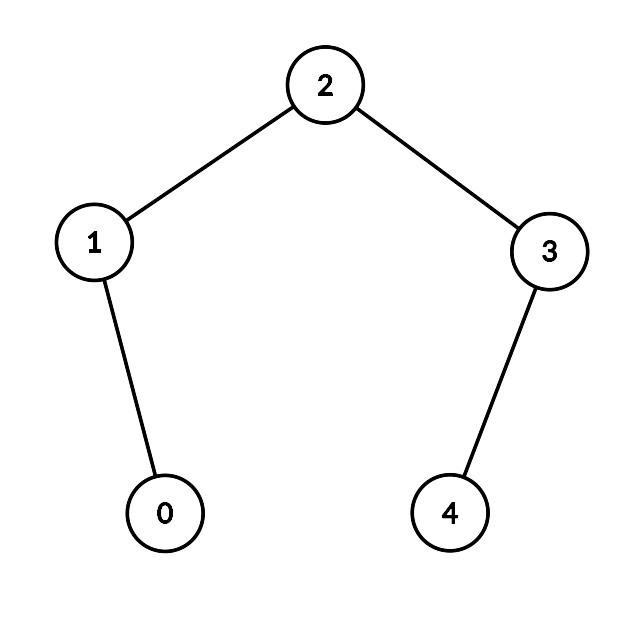
\includegraphics[height=0.15\textheight]{Figures/p5A}
		\caption{}
		\label{subfig:monotonicityA}
	\end{subfigure}
	\hfill
	\begin{subfigure}[t]{0.3\textwidth}
		\centering
		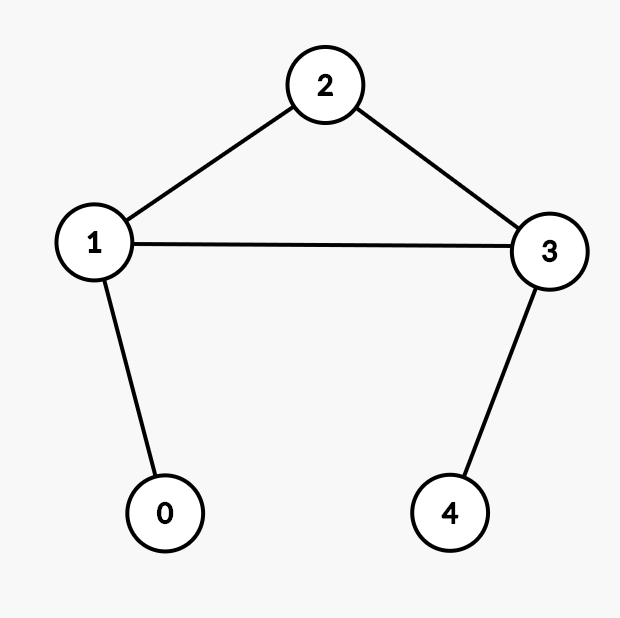
\includegraphics[height=0.15\textheight]{Figures/p5B}
		\caption{}
		\label{subfig:monotonicityB}
	\end{subfigure}
	\vspace{20pt}
	\hfill
	\caption{Edge addition between opposed opinions.}
	\label{fig:p5}
\end{figure}

\begin{equation}
	\begin{aligned}
		\\
		L+I=
		\left(\begin{matrix}
		2 & -1 & 0 & 0 & 0 \\
		-1 & 3 & -1 & 0 & 0 \\
		0 & -1 & 3 & -1 & 0 \\
		0 & 0 & -1 & 3 & -1 \\
		0 & 0 & 0 & -1 & 2
		\end{matrix}\right),
		\qquad \qquad 
		(L+I)^{-1}=
		\left(\begin{matrix}
		\frac{34}{55} & \frac{13}{55} & \frac{1}{11} & \frac{2}{55} & \frac{1}{55} \\
		\frac{13}{55} & \frac{26}{55} & \frac{2}{11} & \frac{4}{55} & \frac{2}{55} \\
		\frac{1}{11} & \frac{2}{11} & \frac{5}{11} & \frac{2}{11} & \frac{1}{11} \\
		\frac{2}{55} & \frac{4}{55} & \frac{2}{11} & \frac{26}{55} & \frac{13}{55} \\
		\frac{1}{55} & \frac{2}{55} & \frac{1}{11} & \frac{13}{55} & \frac{34}{55}
		\end{matrix}\right)
		,
		\\
		\\
		\\
		\\
		\qquad \qquad
		s=
		\left(\begin{matrix}
		-1 \\
		1 \\
		-1 \\
		-1 \\
		1
		\end{matrix}\right)
		,
		\qquad \qquad
		(L+I)^{-1}s=
		\left(\begin{matrix}
		\frac{34}{55} & \frac{13}{55} & \frac{1}{11} & \frac{2}{55} & \frac{1}{55} \\
		\frac{13}{55} & \frac{26}{55} & \frac{2}{11} & \frac{4}{55} & \frac{2}{55} \\
		\frac{1}{11} & \frac{2}{11} & \frac{5}{11} & \frac{2}{11} & \frac{1}{11} \\
		\frac{2}{55} & \frac{4}{55} & \frac{2}{11} & \frac{26}{55} & \frac{13}{55} \\
		\frac{1}{55} & \frac{2}{55} & \frac{1}{11} & \frac{13}{55} & \frac{34}{55}
		\end{matrix}\right)
		\times
		\left(\begin{matrix}
		-1 \\
		1 \\
		-1 \\
		-1 \\
		1
		\end{matrix}\right)
		=
		\left(\begin{matrix}
		\frac{-27}{55} \\
		\frac{1}{55} \\
		\frac{-5}{11} \\
		\frac{-21}{55} \\
		\frac{17}{55}
		\end{matrix}\right)
		\\
		\\
		\\
		\\
		\pi(z) = \frac{||z||_{2}^2}{n} = \frac{\sqrt{(\frac{-27}{55})^2 + (\frac{1}{55})^2 + (\frac{-5}{11})^2 + (\frac{-21}{55})^2 + (\frac{17}{55})^2}^2}{5}= 0.13785123966
	\end{aligned}
\end{equation}
\\
\\
\\
\\
We will now compute the polarization index after the addition of the edge $1\rightarrow3$.
\\
\\
\\
\begin{equation}
	\begin{aligned}
		L+I=
		\left(\begin{matrix}
		2 & -1 & 0 & 0 & 0 \\
		-1 & 4 & -1 & -1 & 0 \\
		0 & -1 & 3 & -1 & 0 \\
		0 & -1 & -1 & 4 & -1 \\
		0 & 0 & 0 & -1 & 2
		\end{matrix}\right),
		\qquad \qquad 
		(L+I)^{-1}=
		\left(\begin{matrix}
		\frac{59}{99} & \frac{19}{99} & \frac{1}{11} & \frac{8}{99} & \frac{4}{99} \\
		\frac{19}{99} & \frac{38}{99} & \frac{2}{11} & \frac{16}{99} & \frac{8}{99} \\
		\frac{1}{11} & \frac{2}{11} & \frac{5}{11} & \frac{2}{11} & \frac{1}{11} \\
		\frac{8}{99} & \frac{16}{99} & \frac{2}{11} & \frac{38}{99} & \frac{19}{99} \\
		\frac{4}{99} & \frac{8}{99} & \frac{1}{11} & \frac{19}{99} & \frac{59}{99}
		\end{matrix}\right)
		,
		\\
		\\
		\\
		\qquad \qquad
		s=
		\left(\begin{matrix}
		-1 \\
		1 \\
		-1 \\
		-1 \\
		1
		\end{matrix}\right)
		,
		\qquad \qquad
		(L+I)^{-1}s=
		\left(\begin{matrix}
		\frac{59}{99} & \frac{19}{99} & \frac{1}{11} & \frac{8}{99} & \frac{4}{99} \\
		\frac{19}{99} & \frac{38}{99} & \frac{2}{11} & \frac{16}{99} & \frac{8}{99} \\
		\frac{1}{11} & \frac{2}{11} & \frac{5}{11} & \frac{2}{11} & \frac{1}{11} \\
		\frac{8}{99} & \frac{16}{99} & \frac{2}{11} & \frac{38}{99} & \frac{19}{99} \\
		\frac{4}{99} & \frac{8}{99} & \frac{1}{11} & \frac{19}{99} & \frac{59}{99}
		\end{matrix}\right)		\times
		\left(\begin{matrix}
		-1 \\
		1 \\
		-1 \\
		-1 \\
		1
		\end{matrix}\right)
		=
		\left(\begin{matrix}
		\frac{-53}{99} \\
		\frac{-7}{99} \\
		\frac{-5}{11} \\
		\frac{-29}{99} \\
		\frac{35}{99}
		\end{matrix}\right)
		\\
		\\
		\\
		\pi(z) = \frac{||z||_{2}^2}{n} = \frac{\sqrt{(\frac{-53}{99})^2 + (\frac{-7}{99})^2 + (\frac{-5}{11})^2 + (\frac{-29}{99})^2 + (\frac{35}{99})^2}^2}{5} = 0.14180185695
	\end{aligned}
\end{equation}
\\
We can see an increase of the polarization index after adding this particular edge. This example was discovered after brute-forcing different graph topologies with different combinations of opinion values.
\\	
\begin{lemma}
The polarization index does not necessarily decrease after an edge addition between opposing views.
\end{lemma}

\section{Polarization in a complete graph}
\label{sec:fullgraph}
\vspace{20pt}
Given a polarized graph $G$ we will compute the polarization index $\pi(z)$ before and after converting the graph $G$ to a full graph. 

\begin{table}[!htb]
 \centering
 \caption{Polarization Before and after converting to a full graph}
 \label{tab:fullgraph}
 \begin{tabular}{| l || l | l | l | l |}
 \hline
  Dataset & Number of Nodes & Number of edges & Average Degree & $\pi(z)$\\
  \hline
  \hline
  Karate Before & $34$ & $78$ & $4.5882$ &  $0.35857$\\
  \hline
  Karate After & $34$ & $561$ & $33$ &  $0.00081$\\
  \hline
  \hline
  Books Before & $105$ & $441$ & $8.4000$ &  $0.44046$\\
  \hline
  Books After & $105$ & $5460$ & $104.0000$ &  $0.00453$\\
  \hline
  \hline
  Blogs Before & $1490$ & $16718$ & $22.4403$ &  $0.27909$\\
  \hline
  Blogs After & $1490$ & $1109308$ & $1489.0040$ &  $0.00030$\\
  \hline
 \end{tabular}
 \end{table}

\vspace{20pt}
We can see the results from the karate, books and blogs datasets at table ~\ref{tab:fullgraph} The results leads us to the following lemma.
\\	
\begin{lemma}
The polarization index does not drop to zero in a fully connected graph.
\end{lemma}


\chapter{Algorithms}
\label{ch:algorithms}


In this section we  consider a greedy algorithm and some heuristics for reducing $\pi(z)$. All the heuristics use the intuition that connecting the most extreme opinions of each community can result in great reduction. 
When a new edge is introduced, the graph structure changes. This leads to changes in the opinion vector $z$.
The recomputation of the $z$ vector is expensive on time due to the computation of the inverse matrix in the $(L+I)^{-1}S$ formula.
This is why we consider two types of algorithms, those that recompute the $z$ vectors and those that do not.
All the heuristics run on $\mathcal{O}(n^2)$. This is due to the fact that they need to explore all edge combinations.

\section{Algorithms that recompute the opinion vector}
\label{sec:recomputeAlgos}

We begin with a Greedy algorithm. Greedy algorithms work in stages and during each stage a choice is made which is locally optimal.
The Greedy algorithm computes the decrease in $\pi(z)$ and selects the edge with the largest decrease every time.
\\
\\
After finding the best edge, the $Greedy$ algorithm adds this edge to the graph. This result in a change of the network structure.
Then a recomputation of the $z$ vector is happening and  the procedure is repeated.To reduce running times, we  use repeated averaging instead of computing the inverse matrix and limit the accuracy of the convergence.

\vspace{30pt}
    		\begin{algorithm}[H]
		
			\caption{Greedy}
			\label{alg:greedyAlgo}
			
			\begin{flushleft}
        				\textbf{INPUT:} Graph $G(V, E)$; $k$ number of edges to add;
				\vspace{6pt} \\
        				\textbf{OUTPUT:} A set $S$ of $k$ edges to be added to $G$ that minimize the polarization \\
				 index $\pi(z)$
			\end{flushleft}
			
			\begin{algorithmic}[1]
				\FOR {$i = 1:k \ $}
				\STATE Compute the opinion vector $z$
					\FOR { each  edge in $|V| \times |V| \textbackslash E$}
						\STATE Compute the decrease of $\pi(z)$ if edge is added to $G$
					\ENDFOR
					\STATE Select the edge with the largest decrease and add it to $G$
				\ENDFOR
				\STATE Return the set of edges that were selected
			\end{algorithmic}
		\end{algorithm}
\vspace{30pt}

\noindent A second heuristic we consider is the $FirstTopGreedy$. Let $X$ be the set of nodes of expressed opinions $\epsilon$ [-1,0) sorted by increasing order and $Y$ the set of nodes of expressed opinions $\epsilon$ (0,1] sorted by decreasing order. This heuristic use the first $k$ nodes of $X$ and $Y$, resulting in  a $k \times k$ smaller search space. This allows the $FirstTopGreedy$ to reduce the amount of time spend searching for the best edge to add. \noindent 
\\
\\
Last we consider two heuristics that choose edges based on the value of the expressed opinion of their nodes. The Distance of their opinions can be defined as $D=|z_u - z_v|$. This heuristic computes the distance between every edge candidate and then chooses to add the edge with the maximum distance.

\begin{algorithm}[htbp]
	\caption{FirstTopGreedy}
	\label{alg:kgreedy}
	
	\begin{flushleft}
        		\textbf{INPUT:} Graph $G(V, E)$; $k$ number of edges to add;\\
		$X$, the set of nodes that their expressed opinions $\epsilon$ [-1,0) sorted by increasing order\\
		$Y$, set of nodes that their expressed opinions $\epsilon$ (0,1]  sorted by decreasing order\\
		\vspace{6pt}
        		\textbf{OUTPUT:} A set $S$ of $k$ edges to be added to $G$ that minimize the polarization \\ index $\pi(z)$
	\end{flushleft}
	
	\begin{algorithmic}[1]
		\STATE $A \leftarrow $ first $k$ items of $X$
		\STATE $B \leftarrow $ first $k$ items of $Y$
		\FOR {$i = 1:k \ $}
			\STATE Compute the opinion vector $z$
			\FOR { each  edge in $|A| \times |B| \textbackslash E$}
				\STATE Compute the decrease of $\pi(z)$ if edge is added to the graph
			\ENDFOR
			\STATE Select the edge with the largest decrease and add it to $G$
		\ENDFOR
		\STATE Return the set of edges that were selected
	\end{algorithmic}
	
\end{algorithm}
		
\clearpage


\begin{algorithm}[H]
	\caption{ExpressedΟpinion}
	\label{alg:expressedOpinion}
	
	\begin{flushleft}
        		\textbf{INPUT:} Graph $G(V, E)$; $k$ number of edges to add\\
		\vspace{6pt}
        		\textbf{OUTPUT:} A set $S$ of $k$ edges to be added to $G$ that minimize the polarization
		\\ index $\pi(z)$
	\end{flushleft}
	
	\begin{algorithmic}[1]
		\FOR {$i = 1:k \ $}
			\STATE Compute the opinion vector $z$
			\STATE Compute the $z$ values
			\FOR { each  edge in $|V| \times |V| \textbackslash E$}
				\STATE Compute the value $D=|z_u - z_v|$.
			\ENDFOR
			\STATE Sort the distance values by decreasing order
			\STATE Add the edge with the biggest distance to $G$
		\ENDFOR
		\STATE Return the set of edges that were selected
	\end{algorithmic}
	
\end{algorithm}

\section{Algorithms that do not recompute the opinion vector}
\label{sec:norecomputeAlgo}

We continue by exploring some heuristics that do not consider the network changes and thus can run more easily in larger datasets.
Computing the $\pi(z)$ is an expensive operation due to the computation of the inverse matrix. At first we can see a variation of the $Greedy$ algorithm. Its implementation is similar to the $Greedy$. We compute the opinion vector only once and we sort the edges according to the decrease. Then we select the top $k$ edges.
\\
\\
We continue by using a variation of the $FirstTopGreedy$. The $FirstTopGreedyBatch$ heuristic. $FirsTopGreedy$  works exactly like $GreedyBatch$ with the difference that the opinion vector is not recomputed. Let $X$ be the set of nodes that their expressed opinions $\epsilon$ [-1,0) sorted by increasing order and $Y$ the set of nodes that their expressed opinions $\epsilon$ (0,1] sorted by decreasing order. This heuristic is taking the first $k$ nodes of $X$ and $Y$, resulting in $k \times k$ nodes.
\clearpage

\begin{algorithm}[H]
		
			\caption{GreedyBatch}
			\label{alg:greedyBatch}
			
			\begin{flushleft}
        				\textbf{INPUT:} Graph $G(V, E)$; $k$ number of edges to add;
				\vspace{6pt}\\
        				\textbf{OUTPUT:} A set $S$ of $k$ edges to be added to $G$ that minimize the polarization \\ index $\pi(z)$
			\end{flushleft}
			
			\begin{algorithmic}[1]
				\STATE Compute the $z$ values
				\FOR { each  edge in $|V| \times |V| \textbackslash E$}
					\STATE Compute the decrease of $\pi(z)$ if edge is added to $G$ 
				\ENDFOR
				\STATE Sort the values computed by decreasing order;
				\STATE Select the $k$ edges with the largest decrease and add it to $G$
				\STATE Return the set of edges that were selected
			\end{algorithmic}
		\end{algorithm}


\begin{algorithm}[H]
	\caption{FirstTopGreedyBatch}
	\label{alg:kgreedy}
	
	\begin{flushleft}
        		\textbf{INPUT:} Graph $G(V, E)$; $k$ number of edges to add;\\
		$X$, the set of nodes that their expressed opinions $\epsilon$ [-1,0) sorted by increasing order\\
		$Y$, set of nodes that their expressed opinions $\epsilon$ (0,1]  sorted by decreasing order\\
		\vspace{6pt}
        		\textbf{OUTPUT:} A set $S$ of $k$ edges to be added to $G$ that minimize the polarization\\
		 index $\pi(z)$
	\end{flushleft}
	
	\begin{algorithmic}[1]
		\STATE $A, B \leftarrow $ first $k$ items of $X$ , $Y$
				\STATE Compute the $z$ values
		\FOR { each  edge in $|A| \times |B| \textbackslash E$}
			\STATE Compute the decrease of $\pi(z)$ if edge is added to the graph
		\ENDFOR
		\STATE Sort the values computed by decreasing order
		\STATE Select the $k$ edges with the largest decrease and add it to $G$
		\STATE Return the set of edges that were selected
	\end{algorithmic}
	
\end{algorithm}
\clearpage

\section{Computing edge probabilities }		
\label{sec:computingEdge}		
\vspace{20pt}
Our objective is to predict whether there would be a link between 2 unconnected nodes. At first we will find the pairs of nodes that don't have a link between them.	
The next step is to label these pairs. This is needed for preparing a training dataset. 
The edges that are present in the graph will be labeled as $1$ (positive samples) and the unconnected node pairs as $0$ (negative samples).		
\\
\\
\\
\noindent After the labelling we will use the node2vec algorithm to extract node features from the graph. For computing the features of an edge we can add up the features of the nodes of that pair. These features will be trained with a logistic regression model. After the model is trained we will obtain the probabilities of an edge being accepted for every edge. We use the default settings for the $Node2Vec$ algorithm and a 80/20 training/test size for the logistic regression model.
\\
\\
\noindent Computing the actual expected decrease in the polarization, and selecting the $k$ best edges is a difficult problem. Our goal is to incorporate the probabilities in the operation of the algorithms. We do not expect that the decrease in the polarization index will improve. We will do this as follows. 
\\
\\
Each algorithm computes a value $Val(u,v)$ for each candidate edge, and selects greedily edges with the best value. We will replace this value in the algorithm by $P(u,v)*Val(u,v)$. The quantity $Val(u,v)$ can be either the polarization decrease or the absolute distance of the expressed opinions of nodes $u$ and $v$. In the case that $Val(u,v)$ is the polarization decrease the product $P(u,v)*Val(u,v)$ corresponds to the expected polarization decrease.
\\
\\
In addition in section~\ref{sec:median}  Finally in section~\ref{sec:all} we display the results of the heuristics and edited heuristics together including a new algorithm called $maxProb$ that chooses an edge if it is among the edges with the highest acceptance probabilities.

\clearpage


%\chapter{Οδηγίες για τη Μορφή της Διατριβής}
\label{ch:Instructions}


\section{Διαδικασία Υποβολής Τελικού Αντίτυπου Διατριβής}
\label{sec:Submission}
Η μορφή αυτή καθιερώθηκε το 2005 και ενημερώθηκε το 2016.\footnote{\url{https://github.com/vvdimako/cseuoi-thesis}.}
Ο φοιτητής θα πρέπει να φέρει τη διατριβή στη μορφή που περιγράφεται, να περάσει την εξέταση, και να κάνει όλες τις απαιτούμενες από τους εξεταστές μετατροπές.
Έπειτα, η διαδικασία που πρέπει να ακολουθήσει είναι η εξής:
\begin{itemize}
	\item Να πάρει την έγκριση του επιβλέποντος για την τελική μορφή της διατριβής (υπογραφή στη φόρμα Δ3).
	\item Να υποβάλλει τη διατριβή στη Σ.Ε.Μ.Σ. για την τελική έγκριση της μορφής (όπως περιγράφεται εδώ) και να προσκομίσει τη φόρμα Δ3 την οποία θα υπογράψει ένα μέλος της επιτροπής.
	\item Να παραδώσει τη διατριβή σε μορφή PDF στο γραφείο Γ17 μαζί με τη φόρμα Δ3.
	\item Να παραλάβει από το γραφείο Γ17 αντίτυπα του εξωφύλλου, τα οποία θα βάλει μπροστά από τη σελίδα τίτλου της διατριβής. H τελευταία σελίδα θα πρέπει να είναι χοντρό λευκό γυαλιστερό χαρτί.
	\item Να παραδώσει τα 3 αντίτυπα για Μεταπτυχιακή Εργασία Εξειδίκευσης ή 5 αντίτυπα για Διδακτορική Διατριβή στο γραφείο Γ17 και να πάρει την υπογεγραμμένη φόρμα Δ3, την οποία θα παραδώσει και στη Γραμματεία μαζί με τα υπόλοιπα έγγραφα για την αποφοίτηση.
\end{itemize}


\section{Διαμόρφωση Κειμένου}
\label{sec:Text}

\subsection{Βασικές Οδηγίες}
\label{subsec:Basic}
Η διατριβή πρέπει να είναι τυπωμένη σε μονή όψη, ενώ το κείμενο πρέπει να είναι εντός των εξής περιθωρίων:
\begin{itemize}
	\item Top: 2.5 cm.
	\item Bottom: 3 cm.
	\item Left: 2.5 cm.
	\item Right: 2.5 cm.
\end{itemize}
Σε όλη τη διατριβή εκτός από τα Σχήματα και τους Πίνακες (συμπεριλαμβανομένων των λεζάντων όμως) πρέπει να χρησιμοποιείται γραμματοσειρά μεγέθους 12 στιγμών.
Οι όροι μπορούν να είναι σε \textit{πλάγια γράμματα}, χρησιμοποιώντας την εντολή \verb|\textit{πλάγια γράμματα}|, συνήθως την πρώτη φορά που χρησιμοποιούνται.
Τα \textbf{έντονα γράμματα} πρέπει να χρησιμοποιούνται μόνο στην περίπτωση που είναι απαραίτητα για την κατανόηση του κειμένου, χρησιμοποιώντας την εντολή \verb|\textbf{έντονα γράμματα}|.

Το κύριο αρχείο είναι το \texttt{SampleThesis.tex}, στο προοίμιο του οποίου θα πρέπει να περάσετε στο πακέτο \texttt{cseuoi-thesis} τις κατάλληλες επιλογές για τη διατριβή σας.
Αν το κείμενο της διατριβής είναι στα Ελληνικά τότε θα πρέπει να περάσετε την επιλογή \texttt{gr}, ενώ αν το κείμενο της διατριβής είναι στα Αγγλικά τότε θα πρέπει να περάσετε την επιλογή \texttt{en}.
Για τη στοιχειοθεσία Μεταπτυχιακής Εργασίας Εξειδίκευσης θα πρέπει να περάσετε την επιλογή \texttt{msc}, ενώ για τη στοιχειοθεσία Διδακτορικής Διατριβής θα πρέπει να περάσετε την επιλογή \texttt{phd}.
Στην περίπτωση της Μεταπτυχιακής Εργασίας Εξειδίκευσης θα πρέπει επιπλέον να περάσετε την κατάλληλη επιλογή για μία από τις εξής εξειδικεύσεις:
\begin{itemize}
	\item Υπολογιστικά Συστήματα: \texttt{systems}.
	\item Θεωρία Επιστήμης Υπολογιστών: \texttt{theory}.
	\item Λογισμικό: \texttt{software}.
	\item Επιστημονικοί Υπολογισμοί: \texttt{scicomp}.
	\item Τεχνολογίες - Εφαρμογές: \texttt{techapps}.
\end{itemize}
Στην περίπτωση της Διδακτορικής Διατριβής δεν περνάτε επιλογή για εξειδίκευση.

Στη συνέχεια του ίδιου αρχείου θα πρέπει να συμπληρώσετε τα στοιχεία σας στις αντίστοιχες εντολές, αφαιρώντας την εντολή \verb|\colorbox{gray}{}|.
Ειδικότερα, τα στοιχεία που θα πρέπει να συμπληρώσετε είναι ο τίτλος της διατριβής, το ονοματεπώνυμο του φοιτητή, ο μήνας και το έτος αποφοίτησης, καθώς και το ονοματεπώνυμο και τη βαθμίδα του επιβλέπων καθηγητή.
Τα παραπάνω στοιχεία θα πρέπει να τα συμπληρώσετε και στα Ελληνικά και στα Αγγλικά προκειμένου να χρησιμοποιηθούν κατάλληλα σε διάφορα σημεία της διατριβής, όπως η σελίδα τίτλου και οι σελίδες με τις περιλήψεις.
Αν κάποια τμήματα της διατριβής σας είναι σκιασμένα, είτε δεν έχετε συμπληρώσει τα αντίστοιχα στοιχεία σας είτε δεν αφαιρέσατε την εντολή \verb|\colorbox{gray}{}| όταν τα συμπληρώσατε.

\subsection{Κεφάλαια}
\label{subsec:Chapters}
Για να ορίσετε τον τίτλο ενός κεφαλαίου, πρέπει να χρησιμοποιήσετε την εντολή \verb|\chapter{Τίτλος Κεφαλαίου}|.
Παρόμοια, για τους τίτλους ενοτήτων χρησιμοποιείτε την εντολή \verb|\section{Τίτλος Ενότητας}|, ενώ για τίτλους υποενοτήτων την εντολή \verb|\subsection{Τίτλος Υποενότητας}|.
Είναι επιθυμητό να εισάγετε και μία ετικέτα κάθε φορά που χρησιμοποιείτε τις παραπάνω εντολές, το οποίο γίνεται με την εντολή \verb|\label{Ετικέτα}|, προκειμένου να μπορείτε να αναφέρεστε στο αντίστοιχο σημείο του κειμένου με την εντολή \verb|\ref{Ετικέτα}|.

To πακέτο \texttt{xgreek}\footnote{\url{https://www.ctan.org/pkg/xgreek?lang=en}.} ορίζει διάφορες χρήσιμες μακροεντολές, οι οποίες επιτρέπουν την εύκολη χρήση χαρακτήρων που είναι δύσκολα προσβάσιμοι από το πληκτρολόγιο.
Μερικές από αυτές τις μακροεντολές είναι οι εξής:
\begin{itemize}
	\item Άνω τόνος (\anwtonos): \verb|\anwtonos|.
	\item Άνω τελεία (\anoteleia): \verb|\anoteleia|.
	\item Σύμβολο του Ευρώ (\euro): \verb|\euro|.
	\item Σύμβολο τοις χιλίοις (\permill): \verb|\permill|.
\end{itemize}

Όταν θεωρείτε ότι είναι απολύτως απαραίτητο, μπορείτε να εισάγετε μία υποσημείωση με την εντολή \verb|\footnote{Αυτή είναι μία υποσημείωση.}|, η οποία εμφανίζεται στο κάτω μέρος της αντίστοιχης σελίδας\footnote{Αυτή είναι μία υποσημείωση.}.
Αν θέλετε να εισάγετε έναν νέο όρο στο ευρετήριο, θα πρέπει να χρησιμοποιήσετε την εντολή\index{νέος όρος} \verb|\index{νέος όρος}|.
Για κάθε υποόρο που θέλετε να προστεθεί σε έναν προηγούμενο όρο, θα πρέπει να χρησιμοποιήσετε την εντολή\index{νέος όρος!υποόρος} \verb|\index{νέος όρος!υποόρος}|.

\subsection{Παραρτήματα}
\label{subsec:Appendices}
Προαιρετικά, μπορείτε να εισάγετε ένα ή περισσότερα παραρτήματα, τα οποία θα βρίσκονται μετά τη βιβλιογραφία και πριν το ευρετήριο.
Σε αντίθεση με τα κεφάλαια της διατριβής, η αρίθμηση των παραρτημάτων γίνεται με κεφαλαίους χαρακτήρες.


\section{Σχήματα}
\label{sec:Figures}
Τα σχήματα και οι λεζάντες τους πρέπει να είναι πάντα κεντραρισμένα και εντός των περιθωρίων του κειμένου.
Για να εισάγουμε ένα σχήμα στο κείμενο, χρησιμοποιούμε τις παρακάτω εντολές:

\begin{verbatim}
\begin{figure}[t]
 \centering
 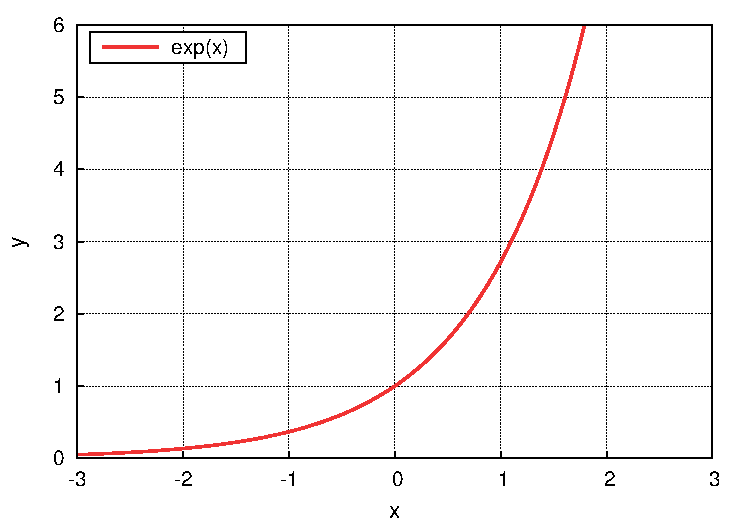
\includegraphics[width=0.65\textwidth]{Figures/ExponentialFunction.pdf}
 \caption{Η εκθετική συνάρτηση.}
 \label{fig:ExponentialFunction}
\end{figure}
\end{verbatim}

\begin{figure}[t]
	\centering
	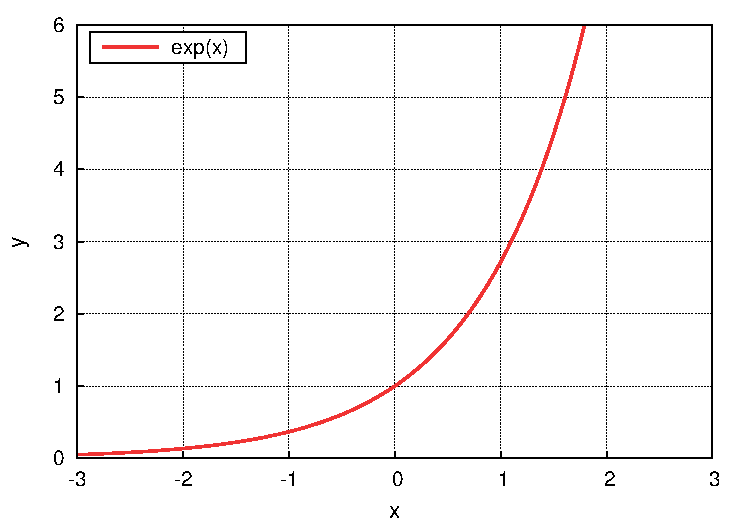
\includegraphics[width=0.65\textwidth]{Figures/ExponentialFunction.pdf}
	\caption{Η εκθετική συνάρτηση.}
	\label{fig:ExponentialFunction}
\end{figure}

Το αποτέλεσμα των παραπάνω εντολών φαίνεται στο Σχήμα~\ref{fig:ExponentialFunction}, ενώ σε περίπτωση που θέλουμε να αναφερθούμε σε αυτό μέσα στο κείμενο, χρησιμοποιούμε την εντολή \verb|Σχήμα~\ref{fig:ExponentialFunction}|.
Αν θέλουμε να εισάγουμε σε ένα σχήμα πολλές εικόνες μαζί, τότε χρησιμοποιούμε τις παρακάτω εντολές:

\begin{verbatim}
\begin{figure}[t]
 \centering
 \begin{subfigure}[t]{0.3\textwidth}
  \centering
  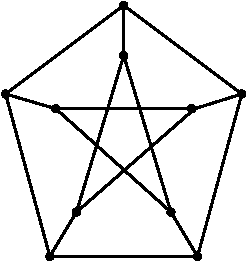
\includegraphics[height=0.15\textheight]{Figures/GraphA.pdf}
  \caption{}
  \label{subfig:GraphA}
 \end{subfigure}
 \hfill
 \begin{subfigure}[t]{0.3\textwidth}
  \centering
  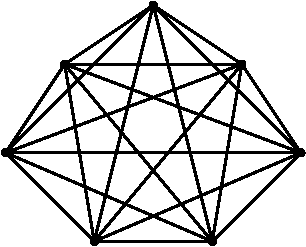
\includegraphics[height=0.15\textheight]{Figures/GraphB.pdf}
  \caption{}
  \label{subfig:GraphB}
 \end{subfigure}
 \hfill
 \begin{subfigure}[t]{0.3\textwidth}
  \centering
  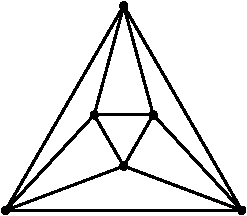
\includegraphics[height=0.15\textheight]{Figures/GraphC.pdf}
  \caption{}
  \label{subfig:GraphC}
 \end{subfigure}
 \caption{Τρία γραφήματα.}
 \label{fig:ThreeGraphs}
\end{figure}
\end{verbatim}

\begin{figure}[t]
	\centering
	\begin{subfigure}[t]{0.3\textwidth}
		\centering
		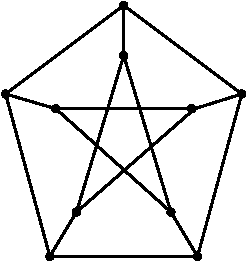
\includegraphics[height=0.15\textheight]{Figures/GraphA.pdf}
		\caption{}
		\label{subfig:GraphA}
	\end{subfigure}
	\hfill
	\begin{subfigure}[t]{0.3\textwidth}
		\centering
		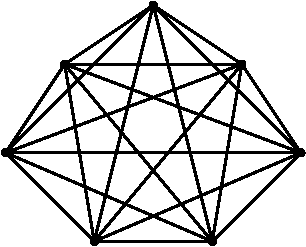
\includegraphics[height=0.15\textheight]{Figures/GraphB.pdf}
		\caption{}
		\label{subfig:GraphB}
	\end{subfigure}
	\hfill
	\begin{subfigure}[t]{0.3\textwidth}
		\centering
		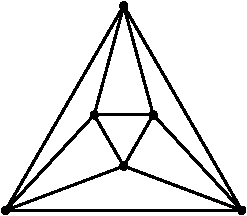
\includegraphics[height=0.15\textheight]{Figures/GraphC.pdf}
		\caption{}
		\label{subfig:GraphC}
	\end{subfigure}
	\caption{Τρία γραφήματα.}
	\label{fig:ThreeGraphs}
\end{figure}

Με τις παραπάνω εντολές εισάγαμε στο Σχήμα~\ref{fig:ThreeGraphs} τρία υποσχήματα, στα οποία μπορούμε να αναφερθούμε και ξεχωριστά αν θέλουμε, χρησιμοποιώντας τις αντίστοιχες ετικέτες που τους αναθέσαμε.


\section{Πίνακες}
\label{sec:Tables}
Με παρόμοιες εντολές μπορούμε να εισάγουμε και πίνακες.
Για παράδειγμα, με τις παρακάτω εντολές δημιουργούμε τον Πίνακα~\ref{tab:Example}.

\begin{verbatim}
\begin{table}[t]
 \centering
 \caption{Ένας Πίνακας.}
 \label{tab:Example}
 \begin{tabular}{| l || l | l | l |}
  \hline
  κελί 1 & κελί 2 & κελί 3 & κελί 4\\
  \hline
  \hline
  κελί 5 & κελί 6 & κελί 7 & κελί 8\\
  \hline
  κελί 9 & κελί 10 & κελί 11 & κελί 12\\
  \hline
  κελί 13 & κελί 14 & κελί 15 & κελί 16\\
  \hline
  κελί 17 & κελί 18 & κελί 19 & κελί 20\\
  \hline
 \end{tabular}
\end{table}
\end{verbatim}

\begin{table}[t]
	\centering
	\caption{Ένας Πίνακας.}
	\label{tab:Example}
	\begin{tabular}{| l || l | l | l |}
		\hline
		κελί 1 & κελί 2 & κελί 3 & κελί 4\\
		\hline
		\hline
		κελί 5 & κελί 6 & κελί 7 & κελί 8\\
		\hline
		κελί 9 & κελί 10 & κελί 11 & κελί 12\\
		\hline
		κελί 13 & κελί 14 & κελί 15 & κελί 16\\
		\hline
		κελί 17 & κελί 18 & κελί 19 & κελί 20\\
		\hline
	\end{tabular}
\end{table}


\section{Αλγόριθμοι}
\label{sec:Algorithms}
Για τη στοιχειοθεσία αλγορίθμων σε μορφή ψευδοκώδικα, όπως φαίνεται στον Αλγόριθμο~\ref{alg:Example} για παράδειγμα, χρησιμοποιούμε τις παρακάτω εντολές:

\begin{verbatim}
\begin{algorithm}[t]
 \caption{Υπολογισμός $y = x^n$.}
 \label{alg:Example}
 \begin{algorithmic}[1]
  \REQUIRE $n \geq 0 \vee x \neq 0$
  \ENSURE $y = x^n$
  \STATE $y \leftarrow 1$
  \IF{$n < 0$}
  \STATE $X \leftarrow 1 / x$
  \STATE $N \leftarrow -n$
  \ELSE
  \STATE $X \leftarrow x$
  \STATE $N \leftarrow n$
  \ENDIF
  \WHILE{$N \neq 0$}
  \IF{$N$ is even}
  \STATE $X \leftarrow X \times X$
  \STATE $N \leftarrow N / 2$
  \ELSE[$N$ is odd]
  \STATE $y \leftarrow y \times X$
  \STATE $N \leftarrow N - 1$
  \ENDIF
  \ENDWHILE
 \end{algorithmic}
\end{algorithm}
\end{verbatim}

\begin{algorithm}[t]
	\caption{Υπολογισμός $y = x^n$.}
	\label{alg:Example}
	\begin{algorithmic}[1]
		\REQUIRE $n \geq 0 \vee x \neq 0$
		\ENSURE $y = x^n$
		\STATE $y \leftarrow 1$
		\IF{$n < 0$}
		\STATE $X \leftarrow 1 / x$
		\STATE $N \leftarrow -n$
		\ELSE
		\STATE $X \leftarrow x$
		\STATE $N \leftarrow n$
		\ENDIF
		\WHILE{$N \neq 0$}
		\IF{$N$ is even}
		\STATE $X \leftarrow X \times X$
		\STATE $N \leftarrow N / 2$
		\ELSE[$N$ is odd]
		\STATE $y \leftarrow y \times X$
		\STATE $N \leftarrow N - 1$
		\ENDIF
		\ENDWHILE
	\end{algorithmic}
\end{algorithm}


\section{Μαθηματικά}
\label{sec:Mathematics}
Για τη στοιχειοθεσία μαθηματικών εκφράσεων χρησιμοποιούμε με παρόμοιο τρόπο τα παρακάτω περιβάλλοντα:
\begin{itemize}
	\item Εξίσωση: \verb|\begin{equation} ... \end{equation}|.

	\begin{equation}
		S_{n} = 1 + \sum_{k=1}^{n}\frac{1}{k^{2} + k}\,,\quad n \in \mathbb{N}\,.
		\label{eq:Example}
	\end{equation}

	\item Θεώρημα: \verb|\begin{theorem} ... \end{theorem}|.

	\begin{theorem}
		Τhe square of the hypotenuse (the side opposite the right angle) is equal to the sum of the squares of the other two sides.
	\end{theorem}

	\item Λήμμα: \verb|\begin{lemma} ... \end{lemma}|.

	\begin{lemma}
		If a prime divides the product of two numbers, it must divide at least one of those numbers.
	\end{lemma}

	\item Πόρισμα: \verb|\begin{corollary} ... \end{corollary}|.

	\begin{corollary}
		In any right triangle, the hypotenuse is greater than any one of the other sides, but less than their sum.
	\end{corollary}

	\item Γεγονός: \verb|\begin{fact} ... \end{fact}|.

	\begin{fact}
		It takes 8 minutes 17 seconds for light to travel from the Sun’s surface to the Earth.
	\end{fact}

	\item Σημείωση: \verb|\begin{remark} ... \end{remark}|.

	\begin{remark}
		This is a remark.
	\end{remark}

	\item Ορισμός: \verb|\begin{definition} ... \end{definition}|.

	\begin{definition}
		Addition is bringing two or more numbers (or things) together to make a new total.
	\end{definition}

	\item Παρατήρηση: \verb|\begin{observation} ... \end{observation}|.

	\begin{observation}
		This is an observation.
	\end{observation}

	\item Aπόδειξη: \verb|\begin{proof} ... \end{proof}|.

	\begin{theorem}[Fermat's Last Theorem]
		There are no positive integers $x$, $y$, and $z$ that satisfy the equation $x^{n} + y^{n} = z^{n}$ for any integer value of $n > 2$.
	\end{theorem}
	\begin{proof}
		``I have discovered a truly marvellous proof of this, which this margin is too narrow to contain.''
	\end{proof}
\end{itemize}


\section{Διαχείριση Βιβλιογραφίας}
\label{sec:Bibliography}
Για τη δημιουργία της βιβλιογραφίας χρησιμοποιούμε το πακέτο BibTeX.
Για αυτό απαιτείται μία βιβλιογραφική βάση δεδομένων, η οποία αποθηκεύεται ως ένα απλό αρχείο κειμένου με κατάληξη bib.
Το αρχείο αυτό περιέχει καταχωρήσεις της παρακάτω μορφής:

\begin{verbatim}
@article{Newman2003a,
 author = {Newman, Mark E. J.},
 title = {The Structure and Function of Complex Networks},
 journal = {SIAM Review},
 volume = {45},
 number = {2},
 pages = {167--256},
 year = {2003},
 doi = {10.1137/S003614450342480}
}
\end{verbatim}

\section{Proposed Algorithm}
\label{sec:proposedAlgorithm}

The results from section~\ref{sec:intuition} makes us consider edge addition between high conflicting value nodes. After making this edge connection between two nodes we will see a big decrease. After this decrease the network will recalculate the expressed opinions since we are using a repeated averaging model. 
\\
\\
These two nodes that were decreased and became more neutral will now start to influence their other neighbours. If their other neighbours have a high value the new calculation will not see a big decrease due to the fact that the smallest decrease is happening when we connect a value near zero and a relatively high value, as we saw in ~\ref{sec:intuition}. To find out we will have to compute the decrease of each high conflicting values and get the best of them. 

The algorithm can be seen in the figure ~\ref{alg:algorithm}.

\begin{algorithm}[t]
	\caption{Minimization of the polarization index $\pi(z)$}
	\label{alg:algorithm}
	\begin{flushleft}
        		\textbf{INPUT:} Graph $G$, number of edges to add , $k$; $k1$, $k2$, High polarization vertices of each opinion, [-1,0] and [0,1], $X$,$Y$ respectively.\\
        		\textbf{OUTPUT:} List of $k$ edges that minimize the polarization index $\pi(z)$
	\end{flushleft}
	\begin{algorithmic}[1]
		\STATE $Out \leftarrow Empty List;$
		\FOR {$i = 1:k1 \ do$}
		\STATE $Vertex \ u = X[i]$
		\FOR {$j= 1:k2 \ do$}
		\STATE $Vertex \ v = Y[i]$
		\STATE Compute $\pi(z)$, the decrease if the edge $(u,v)$ is added;
		\STATE Append edge $(u,v)$ to Out;
		\ENDFOR
		\ENDFOR
		\STATE $Sorted \leftarrow sort(Out)$ by $\pi(z)$ by decreasing order;
		\STATE Return top $k$ from $Sorted$
	\end{algorithmic}
\end{algorithm}
% !TEX TS-program = XeLaTeX
%
% Περάστε στο πακέτο cseuoi-thesis τις κατάλληλες επιλογές για τη διατριβή σας
%
%\documentclass[gr,phd]{cseuoi-thesis} % Διδακτορικό (στα Ελληνικά)
\documentclass[en,msc,systems]{cseuoi-thesis} % Μεταπτυχιακό με εξειδίκευση στα Υπολογιστικά Συστήματα (στα Αγγλικ)ά
%\documentclass[en,msc,theory]{cseuoi-thesis} % Μεταπτυχιακό με εξειδίκευση στη Θεωρία Επιστήμης Υπολογιστών (στα Αγγλικά)
%\documentclass[en,msc,software]{cseuoi-thesis} % Μεταπτυχαικό με εξειδίκευση στο Λογισμικό (στα Αγγλικά)
%\documentclass[en,msc,scicomp]{cseuoi-thesis} % Μεταπτυχιακό με εξειδίκευση στους Επιστημονικούς Υπολογισμούς (στα Αγγλικά)
%\documentclass[en,msc,techapps]{cseuoi-thesis} % Μεταπτυχιακό με εξειδίκευση στις Τεχνολογίες - Εφαρμογές (στα Αγγλικά)


% 
% Συμπληρώστε τα στοιχεία σας στις παρακάτω εντολές (αφαιρώντας το \colorbox{gray}{})
%
\titleEn{Reducing Polarization in Social Media}
\authorEn{Leonidas Boutsikaris}
\arthro{τον}
\aitiatiki{}
\dateEn{February 2021}
\advisorEn{Panayiotis Tsaparas, Assistant Professor}



% 
% Εξεταστική επιτροπή για ΜΔΕ
%
\MSCexaminer{Panayiotis Tsaparas}{Associate Professor}%
    {Department of Computer Science and Engineering, University of Ioannina (Supervisor)}
\MSCexaminer{? ?}{Associate Professor}%
    {Department of Computer Science and Engineering, University of Ioannina }
\MSCexaminer{? ?}{Associate Professor}%
    {Department of Computer Science and Engineering, University of Ioannina }


% Πακέτο για την εμφάνιση περιθωρίων (χρήσιμο για την εύρεση overfull boxes)
%\usepackage{showframe}

% Πακέτο για τη διατήρηση των floats (εικόνες κ.α.) εντός των ενοτήτων
%\usepackage[section]{placeins}



\begin{document}

% Σελίδες χωρίς αρίθμηση
\pagenumbering{gobble}

% Εκτύπωση της σελίδας τίτλου
\maketitle

% Εκτύπωση της σελίδας με τις επιτροπές
\makecommittees

% Αρχικοποίηση του minitoc
\dominitoc[n]

%\chapter*{\cseafierwsi}

Η σελίδα αυτή είναι προαιρετική και περιέχει αφιέρωση σε κάποιο σημαντικό πρόσωπο.

\bigskip

\noindent Προτεινόμενο: 1-2 γραμμές.

\noindent Μέγιστο: 1 σελίδα.
 % Προαιρετικό
%\chapter*{\cseeuxaristies}

Η σελίδα αυτή είναι προαιρετική και περιέχει ευχαριστίες σε άτομα που βοήθησαν με οποιονδήποτε τρόπο τον συγγραφέα της διατριβής.

\bigskip

\noindent Προτεινόμενο: 10-15 γραμμές.

\noindent Μέγιστο: 1 σελίδα. % Προαιρετικό


% Σελίδες με αρίθμηση i, ii, iii, iv, ...
\pagenumbering{roman}

% Περιεχόμενα
\pdfbookmark{\contentsname}{contents} % hyperref
\tableofcontents

% Κατάλογος Σχημάτων
%\addstarredchapterc{\listfigurename} % minitoc
%\listoffigures

% Κατάλογος Πινάκων
%\addstarredchapterc{\listtablename} % minitoc
%\listoftables

% Κατάλογος Αλγορίθμων
%\addstarredchapterc{\listalgorithmname} % minitoc
%\listof{algorithm}{\listalgorithmname}

%\chapter*{\glossaryname}
% Εισαγωγή του κεφάλαιου στα περιεχόμενα
\addstarredchapter{\glossaryname} %minitoc

Η σελίδα αυτή είναι προαιρετική.
Περιέχει ορισμούς και επεξηγήσεις εννοιών, όρων, συντομεύσεων, και συμβολισμών.
Αν η έκτασή τους είναι μεγαλύτερη από δύο σελίδες τότε πρέπει να πάει στο τέλος της διατριβής, αμέσως μετά τα παραρτήματα. % Προαιρετικό

% Περίληψη και εκτεταμένη περίληψη
%\chapter*{\abstractname}
\addstarredchapter{\abstractname} % minitoc

\noindent We know for a fact that opinions are formed through social interactions. Online communities offer public access to social disputes on controversial matters that allow the study and moderation of them. The majority of studies in social networks are based on the Friedkin-Johnsen model.
\\
\\
Users of online communities are receiving biased information that amplify their own viewpoints. This creates a fragmented community and users interact only with individuals that hold the same opinions. In this thesis we use the polarization index to measure the polarization of a social graph.
\\
\\We try to reduce the polarization by connecting individuals. We propose new social connections between different and extreme opinions by following the intuition of the Friedkin-Johnsen model. 
\\
\\
Finally, probabilities are adopted to our heuristic algorithms that now make selections based on how probable is the acceptance of a recommendation of a new social connection. 

\bigskip

%\chapter*{\cseextabstract}
\addstarredchapter{\cseextabstract} % minitoc

%\makecseextabstract


\noindent Εκτεταμένη περίληψη της εργασίας στην αντίθετη γλώσσα από αυτήν του κειμένου.
Αν το κείμενο είναι στα Ελληνικά τότε αυτή η σελίδα πρέπει να είναι στα Αγγλικά.
Αν το κείμενο είναι στα Αγγλικά τότε αυτή η σελίδα πρέπει να είναι στα Ελληνικά.

\bigskip

\noindent Προτεινόμενο: 2 σελίδες.

\noindent Μέγιστο: 4 σελίδες.


% Σελίδες με αρίθμηση 1, 2, 3, 4, ...
\pagenumbering{arabic}


% Εισαγωγή των κεφαλαίων
\chapter{Introduction and the Theory Behind Polarization}
\label{ch:Introduction}


\section{Introduction}
\label{sec:Objectives}

Polarization describes the division of people into two contrasting groups or sets of opinions or beliefs. The term is used in various domains such as politics and social studies. For example political polarization refers to the divergence of political attitudes to ideological extremes. Social studies use this term to  describe the segregation within a society in terms of income inequality or social and class status. Currently social media have a big role as a source of news and information and a lot of the related discussions of people have gone online. Polarization is linked with harmful effects such as intensifying stereotypes and creating echo chambers. In echo chambers individuals get their news only from like-minded people as they share and reinforce one another’s opinions. Additionally the fact that people tend to ignore opposing views in combination with algorithmic personalization results a significant increase of polarization.

\section{Social and Psychological Factors}

Individuals experience discomfort when given data that actively challenge their opinions. In the field of psychology, cognitive dissonance occurs when a person holds two or more contradictory beliefs, ideas, or values and experiences psychological stress because of that. In simple terms dissonance is defined as a the lack of agreement.
Individuals want to reduce the discomfort that is caused from cognitive dissonance. Reduction occurs by strengthening opinions that come in agreement with their own and downplaying everything that challenges them. This leads individuals to a selective exposure on information \cite{jonasHardtFreyThelen2001}. Selective exposure is also demonstrated in groups. Furthermore people assign themselves with social identities. The self-categorization theory stems from the social identity theory, which holds that conformity stems from psychological processes. Accordingly, proponents of the self-categorization model hold that group polarization occurs because individuals identify with a particular group and conform to a prototypical group position that is more extreme than the group mean. It is shown that groups of people tend to make decisions that are more extreme than the initial inclination of its members \cite{sunstein}.

\label{sec:Structure}

\section{Polarization online}

Online entities such as news or social media platforms are aware of their users opinions  and aim to maximize their satisfaction. As discussed above, platforms will present content in a way that minimizes psychological stress. This leads to media bias. Media bias is the bias or perceived bias of journalists and news producers within the mass media in the selection of many events and stories that are reported and how they are covered. When this happens online, personalization of the content creates algorithmic bias. Algorithmic bias describes systematic and repeatable errors in a computer system that create unfair outcomes, such as privileging one arbitrary group of users over others. Bias can emerge due to many factors like the design of the algorithm. Due to personalization we don't see the same content and this is the main reason for the formation of filter bubbles.

\section{Filter Bubbles}

Filter bubbles are the echo chambers of social media. In news media, an echo chamber is a metaphorical description of a situation in which beliefs  and opinions are strengthened by communication and repetition inside a closed system. It is important to distinguish the difference between echo chambers and filter bubbles. This two concepts are almost identical, however,  filter bubbles are a result of algorithms that choose content based on previous online behaviour, as with search histories or online shopping activity.



\chapter{Related Work}
\label{ch:Instructions}


\section{Measuring the Polarization of a Network}
\label{sec:Submission}

At first we have to measure the opinion polarization in a social Network. The actions and information of a user can give us insights about his opinions on a topic e.g. accounts a user follows, content they repost, comments they make , etc. Using this information we can measure the polarization. 
\\
\\
Assume a graph $G = (V,E)$ representing a network that is connected and undirected. $Z$ will be the vector of expressed opinions for the whole network. Each value $Z_i$ of the vector will represent a node and can be computed with the opinion-formation model of Friedkin and Johnsen. 
\\
\\
The length of the opinion vector $||z|| ^2$ measures  the polarization and  $\pi(z) = \frac{||z|| ^2}n$ is defined as the polarization index of the network, where  $n$ is the number of nodes in the graph so the polarization index can be independent of the network size. 
\\
\\
There is a direct link between this opinion model and random walks. Given the graph $G = (V,E)$ we can construct the augmented graph $H(V∪X, E∪R)$. For each vertex of  $V$ we will add a new vertex on $X$ and a directed edge $(v_i,x_i)$ in $R$. 
\\
\\
The node $x_i$ corresponds to the internal opinion of the node $v_i$. In the model we follow $z_j$ or else the expressed opinion of a user that can be computed by the probability of $P(x_i |v_j)$. This probability represents that a random walk on the augmented graph that started from the node $V_j$ ended at the node $X_i$ or else how much likely the probability of user $V_j$ adopting the opinion of user $V_i$. This probability depends on the structure of the graph. 
\\
\\
Two problems are introduced, the $ModerateInternal$ and the $ModerateExpressed$. When moderating opinions a small set of nodes $T_s$ is being set to zero, in each problem, as their names suggests, internal or external opinions are set to zero. Two algorithms are proposed for the $ModerateInternal problem$. 
\\
\\
A greedy algorithm that finds the set $T_s$ of nodes iteratively according to the biggest decrease it causes and the Binary Orthogonal Matching Pursuit (BOMP) algorithm. For the $ModerateExpressed$ problem the same greedy algorithm is used.
\cite{tsapMatakosTerzi}


\section{Polarization and Disagreement}
\label{sec:polarizationDisareement}

Another way of looking at polarization is by combining it with disagreement. The main problem of minimising polarization and disagreement lies in the opinions of each user and how targeted ads and recommendations influence their opinions. 
\\
\\
Considering the disagreement in combination with polarization a network can choose how to respond in different situations. Their recommendation system could choose between keeping the disagreement low or exposing users to radically different opinions. There are situations that this optimisation can reduce the overall polarization-disagreement in the network by recommending edges in different parts of the network than the ones that agree with the human confirmation bias. 
\\
\\
Given a social network $G = (V,E,w)$ and initial opinions $s: V \rightarrow [0,1]$ the equilibrium vector according to the Friedkin-Johnsen model is defined as $z^*=(I+L)^1s$ where $L$ is the laplacian matrix of the graph and $I$ the identity matrix. Disagreement of $d(u,v)$ of edge $(u,v)$ is defined as the squared difference between the opinions of $u,v$ at equilibrium: $d(u,v) = w_{uv}(Z_u^* - Z_v*)^2.$ 
\\
\\
The total disagreement is defined as $D_{G,s} = \sum_{(u,v) \epsilon E} d(u,v)$. With $\bar z = z^* - \frac{z*^T \overrightarrow 1}{n}\overrightarrow 1$ polarization is measured as a deviation from the average with the standard definition of variance as $P_{G,s} = \sum_{u\epsilon V} \bar z_u^2 = \bar z^T \bar z$ .
\\
\\
The polarization-disagreement index is defined as follows $I_{G,s} = P_{G,s} +D_{G,s}$. The objective is to minimize this index. 
\\
\\
Muco and Tsourakakis have shown that minimising $\bar z^T \bar z + \bar z^T L\bar z$ is the same to minimising the polarization-disagreement index. Here, $L$ is a matrix among the set of valid combinatorial Laplacians of connected graphs.\cite{musco}

\section{Quantifying and minimizing Risk of Conflict in Social Networks}
\label{sec:riskOfConflict}

We know for a fact that opinions are formed through social interactions and in every interaction conflict arises. Online networks offer public access to social disputes on controversial matters that allows the study and moderation of them. The majority of studies are based in the Friedkin-Johnsen model. 
\\
\\
The main problem is with the Friedkin-Johnsen model metrics. The external opinion of a user, which by definition is hard to measure, combined with the internal opinion which is impossible to be measured. Another problem occurs in the editing of the social graph. We edit the social graph in a way that minimises the conflict of a certain social issue. This can lead to an increased conflict of one or more social issues inside the network.
\\
\\
\\
Chen, Lijffijt and De Bie still use the Friedkin-Johnsen model to evaluate the network conflict but the quantifications depend only on the network topology in a way that the conflict can be reduced over all issues. Worst-case(WCR) conflict risk and average-case conflict risk(ACR) are defined to represent two separate problems, how the network can be minimised in the worst case or in the average case scenario by altering the social graph. 
\\
\\
These problems consider the measures of internal conflict, external conflict, and controversy. Internal conflict ($ic$) measures the difference of the internal and the expressed opinion of a user. $ic = \sum_i{(z_i-s_i)^2}.$
\\
\\
 External conflict ($ec$) measures how different are the opinions of the neighbours with each other. $ec = \sum_{(i,j) \epsilon E}{w_{ij}(z_i-z_j)^2}$. 
 \\
 \\
 Controversy ($c$) measures the variation of the opinions in the network and is independent of the social graph structure. $c = \sum_i{z_i}^2.$
 \\ 
 \\
 These measures are not independent. Reducing one of them results in the increase of another. This leads to the conservation law of conflict. $S^TS = ic + 2ec +  c.$ 
 \\
 \\
 There are two methods of minimising the conflict of the network for each of the ACR and WCR problems. One is a gradient method that  considers deleting and adding edges simultaneously and the other is a descent method that suggests deleting or adding a single edge. Chen, Lijffijt and De Bie used small world random networks and random networks with binomial and power law degree distribution to find out what types of networks have the highest risks for every conflict measure they defined. 
 \\
 \\
 A small world network is a type of graph in which most nodes are not neighbours of one another, but the neighbours of any given node are likely to be neighbours of each other and most nodes can be reached from every other node by a small number of hops or steps. They found that the small world networks are the most high-risk for the $ic$ metric. For $c$ and $r$ the most high-risk network depends on the density.\cite{chen}

\section{Reducing Controversy by connecting Opposing Views}
\label{sec:reducing}

Garimella et al. relly on a measure of controversy that is shown to work reliably in multiple domains in contrast with other measures that focus on a single topic. The controversy measure consists of the following steps:

\begin{enumerate}
  \item Given a topic $t$ they create an endorsement gragp $G=(V,E)$. This graph represents users who have generated content relevant to $t$. For example hashtags of a user.
  
  \item The nodes of this graph a re partitioned in two disjoint sets $X$ and $Y$. The partition is obtained using a graph-partition algorithm.
  
  \item The last step, is computing the controversy measure through a random-walk, thus creating the controversy score $RWC$. This score is defined as the difference of the probability that a random walk starting on one side of the partition will stay on the same side and the probability that the random walk will cross to the other side. A personalized PageRank is used where the restart probabilities are set to a random vertex of each side.
\end{enumerate}
\vspace{4pt}
Garimella et al. states that real graphs often have a star-like structure. Small number of higly popular vertices have a lot of incoming edges. These nodes can be seen as thought leaders and their followers. It is shown that connecting the high degree vertices minimises the $RWC$ score.
\\
\\
Probabilities are also incorporated in the sense that a new edge addition may be not accepted by the user. The polarity here is defined as $R_u= p^X(u) - p^Y(u) \epsilon [-1,1]$. 
\\
\\
The definition of $p^X(u)$ and $p^Y(u)$ is the fraction of other vertices $u'$ for which $lu'^X<lu^X$ and $lu'^Y<lu^Y$. 
\\
\\
In addition $lu^X$ and $lu^Y$ stand for the expected time a random walk needs to hit the high degree vertices of $X$ and $Y$ respectively starting from u. Considering $u$ and $v$ as 2 different and not connected users $P(u, v)$ is defined as the probability that $u$ accepts a recommendation to connect with $v$.
 \\
 \\
 Let $R_u$ and $R_v$ the polarity of these users respectively. $P(u, v)$ is estimated from the training data by obtaining $N_{Endorsed(R_u,R_v)} / N_{Exposed(R_u,R_v)}$.
 \\
 \\
The $Endorsed(R_u,R_v)$ and $Exposed(R_u,R_v)$ values represent the number of times a user with polarity $R_v$ was exposed/endorsed content generated by a user with $R_u$. For example $v$ follows $u$, thus $v$ is exposed to all content $u$ generates.
\\
\\ 
Finally we can re-define the problem as the expected decrease of $RWC$.
$E(u,v) = p(u,v) * δRWC_{u \rightarrow v}$


\chapter{Premilinaries and Problem Definition}
\label{ch:premAndDef}


\section{The Friedkin and Johnsen Model}
\label{sec:prem}

The model will use the information about the opinion of the user, internal and external, but also the constant update of the external opinions of the neighbourhood of the user e.g. the friend list or the accounts the user follows
to compute an opinion vector. This vector is a metric for the whole social graph that can give us insight about its current situation. The vector values range from [-1,1]. Values closer to the range limits indicate bigger polarization. Polarized graphs create groups of nodes that are strongly connected with each other and feedback to one another the same extreme opinion over a topic. These groups can be seen clearly in the illustration of filter bubbles and often associated with politics and controversial issues of our society. Using a certain number of users we can achieve a reduction on the polarization of the network. 
\\
\\
\\
We can educate a group of users with the opposite view, and in terms of our model that means that we can modify the social graph by adding a connection between  users of different opinions. \\
\\
Let $G = (V,E)$ be a connected undirected graph representing a network. Let $z$ be the vector of expressed opinions  for the whole network. Each value  of the vector represents a node and can be computed with the opinion-formation model of Friedkin and Johnsen as follows. 

\begin{equation} 
	z_i = \frac{w_{ii}*si + \sum_{j \epsilon N(i) }{w_{ij}*z_j}} {w_{ii} + \sum_{j \epsilon N(i) }{w_{ij}}} 
\end{equation} 
\\
Where $s_i$ denotes the internal and $z_i$ the expressed opinion of a user. The internal opinion of a user corresponds to the views that inherently has for a controversial topic while the expressed one is the views that the user shares on a social network with his neighbours. The length of the opinion vector $||z|| ^2$ measures  the polarization of the network. To make the polarization  independent of its network we can  normalize it  by dividing  it with the length of the vector $z$. 
An equivalent way of obtaining the vector $z$ from a graph is the following: if $L$ is the laplacian matrix of a graph $G=(V,E)$, and $I$ is the identity matrix, then $z=(L+I)^{-1}S$ \cite{bindel}. 

\section{Measuring the polarization}
\label{sec:meas}

We measure the polarization by its distance from a neutral opinion. We can quantify this with the length of the vector of the second norm $L_{2}^2$ \cite{tsapMatakosTerzi}.

\begin{equation}
	\pi(z) = ||z||_{2}^2
\end{equation}
\\
This value can be independent of the network if we normalize it by dividing with the size of the graph.


\section{A small example of the Friedkin and Johnsen Model}
\label{sec:example}
We will now present a small example so we can build a basic understanding of the Friedkin and Johnsen Model. Consider a small graph that consists of two nodes, $u$ and $v$ with internal opinions of 1 and -1 and $w_{uu} = w_{vu} = w_{vv} = 1$.

\begin{equation} 
	 z_u = \frac{1*1 + 1*1 + 1*(-1)}{1 + 2} = \frac{1}{3} \quad, \quad
	 z_v = \frac{1*(-1) + 1*(-1) + 1*1}{1 + 2} = -\frac{1}{3}
\end{equation}

\begin{equation}
	\pi(z) = ||z||_{2}^2 = \sqrt{(\frac{1}{3})^2 + (-\frac{1}{3})^2}^2 = \frac{2}{9}			   
\end{equation}

We did not normalize the polarization index here by dividing with the size of the graph as we have a simple example.

\section{Problem Definition}
\label{sec:problemDef}

Real world events such as Brexit and the 2016 U.S. presidential elections gives us a clear hint about the polarization our society is witnessing. Social media polarization has a strong effect on politics, opinion formation and how people interact with each other in a society. Users of social media are now receiving biased information that amplify their own viewpoints. Enclosed in their filter bubble, they will ignore everyone else and only acknowledge opinions that fit their own reality. In combination with fake news a malicious entity could use social media as a tool to polarize certain groups of people for their own interest. Problem 3 and 4 examine this case. Reducing online polarization is crucial, Problem 1 and 2 can help combat this phenomenon.
\\
\\
\textit{Problem 1}. Let $C \subseteq	V \times V$ a set of edges that are not in the graph. We want to find a subset of $S \subseteq C$ of $k$ edges whose addition to a graph $G$ leads to the greatest reduction of $\pi(z)$.
\\
\\
\\
\textbf{Problem 2}. Let $S$ a set of edges that are proposed for addition in the graph $G$ from \textbf{Problem 1}. We want to find the probabilities of these changes being accepted.
\\
\\
\\
\textbf{Problem 3}. Let $V \times V$ the set of edges of graph $G$. We want to find a subset of edges $S = k, k \in V \times V$   whose removal from the graph $G$ leads to the greatest increase of $\pi(z)$.
\\
\\
\\
\textbf{Problem 4}. Let $S$ the set of edges that are proposed for removal in the graph $G$ from \textbf{Problem 3}. We want to find the probabilities of these changes being accepted.
\\

\section{Monotonicity of the Problem}
\label{sec:monotonicity}
\vspace{20pt}
We observe that $\pi(z)$ is not monotone with respect to the edge additions. This means that adding an edge will not necessarily decrease the polarization index. We will  show that this is true with a counter example. In the network~\ref{fig:p5} nodes 0, 2 and 3 have a value of $s_i=-1$, and nodes 2 and 4 have a value of $s_i=+1$. For both examples we assume that $w_{ii}=w_{ij}=w_{ji}=1$ and $n$ the number of nodes.
We will now compute the polarization index of the original graph
\\
\\
\begin{figure}[h]
	\centering
	\begin{subfigure}[t]{0.3\textwidth}
		\centering
		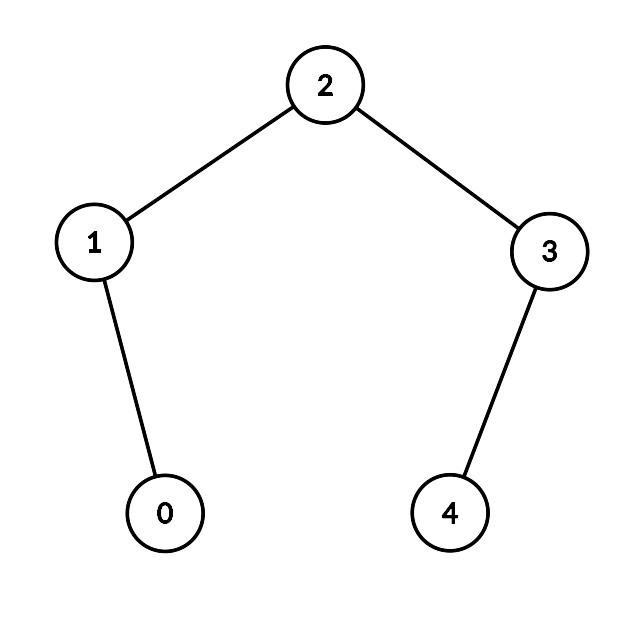
\includegraphics[height=0.15\textheight]{Figures/p5A}
		\caption{}
		\label{subfig:monotonicityA}
	\end{subfigure}
	\hfill
	\begin{subfigure}[t]{0.3\textwidth}
		\centering
		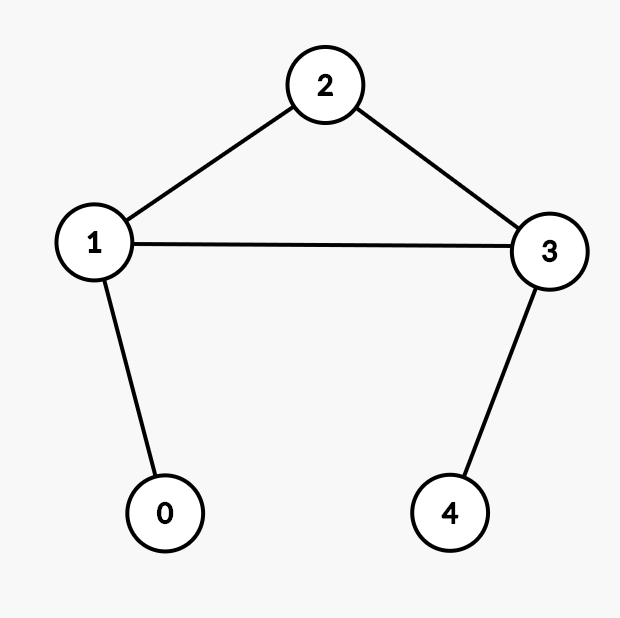
\includegraphics[height=0.15\textheight]{Figures/p5B}
		\caption{}
		\label{subfig:monotonicityB}
	\end{subfigure}
	\vspace{20pt}
	\hfill
	\caption{Edge addition between opposed opinions.}
	\label{fig:p5}
\end{figure}

\begin{equation}
	\begin{aligned}
		\\
		L+I=
		\left(\begin{matrix}
		2 & -1 & 0 & 0 & 0 \\
		-1 & 3 & -1 & 0 & 0 \\
		0 & -1 & 3 & -1 & 0 \\
		0 & 0 & -1 & 3 & -1 \\
		0 & 0 & 0 & -1 & 2
		\end{matrix}\right),
		\qquad \qquad 
		(L+I)^{-1}=
		\left(\begin{matrix}
		\frac{34}{55} & \frac{13}{55} & \frac{1}{11} & \frac{2}{55} & \frac{1}{55} \\
		\frac{13}{55} & \frac{26}{55} & \frac{2}{11} & \frac{4}{55} & \frac{2}{55} \\
		\frac{1}{11} & \frac{2}{11} & \frac{5}{11} & \frac{2}{11} & \frac{1}{11} \\
		\frac{2}{55} & \frac{4}{55} & \frac{2}{11} & \frac{26}{55} & \frac{13}{55} \\
		\frac{1}{55} & \frac{2}{55} & \frac{1}{11} & \frac{13}{55} & \frac{34}{55}
		\end{matrix}\right)
		,
		\\
		\\
		\\
		\\
		\qquad \qquad
		s=
		\left(\begin{matrix}
		-1 \\
		1 \\
		-1 \\
		-1 \\
		1
		\end{matrix}\right)
		,
		\qquad \qquad
		(L+I)^{-1}s=
		\left(\begin{matrix}
		\frac{34}{55} & \frac{13}{55} & \frac{1}{11} & \frac{2}{55} & \frac{1}{55} \\
		\frac{13}{55} & \frac{26}{55} & \frac{2}{11} & \frac{4}{55} & \frac{2}{55} \\
		\frac{1}{11} & \frac{2}{11} & \frac{5}{11} & \frac{2}{11} & \frac{1}{11} \\
		\frac{2}{55} & \frac{4}{55} & \frac{2}{11} & \frac{26}{55} & \frac{13}{55} \\
		\frac{1}{55} & \frac{2}{55} & \frac{1}{11} & \frac{13}{55} & \frac{34}{55}
		\end{matrix}\right)
		\times
		\left(\begin{matrix}
		-1 \\
		1 \\
		-1 \\
		-1 \\
		1
		\end{matrix}\right)
		=
		\left(\begin{matrix}
		\frac{-27}{55} \\
		\frac{1}{55} \\
		\frac{-5}{11} \\
		\frac{-21}{55} \\
		\frac{17}{55}
		\end{matrix}\right)
		\\
		\\
		\\
		\\
		\pi(z) = \frac{||z||_{2}^2}{n} = \frac{\sqrt{(\frac{-27}{55})^2 + (\frac{1}{55})^2 + (\frac{-5}{11})^2 + (\frac{-21}{55})^2 + (\frac{17}{55})^2}^2}{5}= 0.13785123966
	\end{aligned}
\end{equation}
\\
\\
\\
\\
We will now compute the polarization index after the addition of the edge $1\rightarrow3$.
\\
\\
\\
\begin{equation}
	\begin{aligned}
		L+I=
		\left(\begin{matrix}
		2 & -1 & 0 & 0 & 0 \\
		-1 & 4 & -1 & -1 & 0 \\
		0 & -1 & 3 & -1 & 0 \\
		0 & -1 & -1 & 4 & -1 \\
		0 & 0 & 0 & -1 & 2
		\end{matrix}\right),
		\qquad \qquad 
		(L+I)^{-1}=
		\left(\begin{matrix}
		\frac{59}{99} & \frac{19}{99} & \frac{1}{11} & \frac{8}{99} & \frac{4}{99} \\
		\frac{19}{99} & \frac{38}{99} & \frac{2}{11} & \frac{16}{99} & \frac{8}{99} \\
		\frac{1}{11} & \frac{2}{11} & \frac{5}{11} & \frac{2}{11} & \frac{1}{11} \\
		\frac{8}{99} & \frac{16}{99} & \frac{2}{11} & \frac{38}{99} & \frac{19}{99} \\
		\frac{4}{99} & \frac{8}{99} & \frac{1}{11} & \frac{19}{99} & \frac{59}{99}
		\end{matrix}\right)
		,
		\\
		\\
		\\
		\qquad \qquad
		s=
		\left(\begin{matrix}
		-1 \\
		1 \\
		-1 \\
		-1 \\
		1
		\end{matrix}\right)
		,
		\qquad \qquad
		(L+I)^{-1}s=
		\left(\begin{matrix}
		\frac{59}{99} & \frac{19}{99} & \frac{1}{11} & \frac{8}{99} & \frac{4}{99} \\
		\frac{19}{99} & \frac{38}{99} & \frac{2}{11} & \frac{16}{99} & \frac{8}{99} \\
		\frac{1}{11} & \frac{2}{11} & \frac{5}{11} & \frac{2}{11} & \frac{1}{11} \\
		\frac{8}{99} & \frac{16}{99} & \frac{2}{11} & \frac{38}{99} & \frac{19}{99} \\
		\frac{4}{99} & \frac{8}{99} & \frac{1}{11} & \frac{19}{99} & \frac{59}{99}
		\end{matrix}\right)		\times
		\left(\begin{matrix}
		-1 \\
		1 \\
		-1 \\
		-1 \\
		1
		\end{matrix}\right)
		=
		\left(\begin{matrix}
		\frac{-53}{99} \\
		\frac{-7}{99} \\
		\frac{-5}{11} \\
		\frac{-29}{99} \\
		\frac{35}{99}
		\end{matrix}\right)
		\\
		\\
		\\
		\pi(z) = \frac{||z||_{2}^2}{n} = \frac{\sqrt{(\frac{-53}{99})^2 + (\frac{-7}{99})^2 + (\frac{-5}{11})^2 + (\frac{-29}{99})^2 + (\frac{35}{99})^2}^2}{5} = 0.14180185695
	\end{aligned}
\end{equation}
\\
We can see an increase of the polarization index after adding this particular edge. This example was discovered after brute-forcing different graph topologies with different combinations of opinion values.
\\	
\begin{lemma}
The polarization index does not necessarily decrease after an edge addition between opposing views.
\end{lemma}

\section{Polarization in a complete graph}
\label{sec:fullgraph}
\vspace{20pt}
Given a polarized graph $G$ we will compute the polarization index $\pi(z)$ before and after converting the graph $G$ to a full graph. 

\begin{table}[!htb]
 \centering
 \caption{Polarization Before and after converting to a full graph}
 \label{tab:fullgraph}
 \begin{tabular}{| l || l | l | l | l |}
 \hline
  Dataset & Number of Nodes & Number of edges & Average Degree & $\pi(z)$\\
  \hline
  \hline
  Karate Before & $34$ & $78$ & $4.5882$ &  $0.35857$\\
  \hline
  Karate After & $34$ & $561$ & $33$ &  $0.00081$\\
  \hline
  \hline
  Books Before & $105$ & $441$ & $8.4000$ &  $0.44046$\\
  \hline
  Books After & $105$ & $5460$ & $104.0000$ &  $0.00453$\\
  \hline
  \hline
  Blogs Before & $1490$ & $16718$ & $22.4403$ &  $0.27909$\\
  \hline
  Blogs After & $1490$ & $1109308$ & $1489.0040$ &  $0.00030$\\
  \hline
 \end{tabular}
 \end{table}

\vspace{20pt}
We can see the results from the karate, books and blogs datasets at table ~\ref{tab:fullgraph} The results leads us to the following lemma.
\\	
\begin{lemma}
The polarization index does not drop to zero in a fully connected graph.
\end{lemma}


\chapter{Algorithms}
\label{ch:algorithms}


In this section we  consider a greedy algorithm and some heuristics for reducing $\pi(z)$. All the heuristics use the intuition that connecting the most extreme opinions of each community can result in great reduction. 
When a new edge is introduced, the graph structure changes. This leads to changes in the opinion vector $z$.
The recomputation of the $z$ vector is expensive on time due to the computation of the inverse matrix in the $(L+I)^{-1}S$ formula.
This is why we consider two types of algorithms, those that recompute the $z$ vectors and those that do not.
All the heuristics run on $\mathcal{O}(n^2)$. This is due to the fact that they need to explore all edge combinations.

\section{Algorithms that recompute the opinion vector}
\label{sec:recomputeAlgos}

We begin with a Greedy algorithm. Greedy algorithms work in stages and during each stage a choice is made which is locally optimal.
The Greedy algorithm computes the decrease in $\pi(z)$ and selects the edge with the largest decrease every time.
\\
\\
After finding the best edge, the $Greedy$ algorithm adds this edge to the graph. This result in a change of the network structure.
Then a recomputation of the $z$ vector is happening and  the procedure is repeated.To reduce running times, we  use repeated averaging instead of computing the inverse matrix and limit the accuracy of the convergence.

\vspace{30pt}
    		\begin{algorithm}[H]
		
			\caption{Greedy}
			\label{alg:greedyAlgo}
			
			\begin{flushleft}
        				\textbf{INPUT:} Graph $G(V, E)$; $k$ number of edges to add;
				\vspace{6pt} \\
        				\textbf{OUTPUT:} A set $S$ of $k$ edges to be added to $G$ that minimize the polarization \\
				 index $\pi(z)$
			\end{flushleft}
			
			\begin{algorithmic}[1]
				\FOR {$i = 1:k \ $}
				\STATE Compute the opinion vector $z$
					\FOR { each  edge in $|V| \times |V| \textbackslash E$}
						\STATE Compute the decrease of $\pi(z)$ if edge is added to $G$
					\ENDFOR
					\STATE Select the edge with the largest decrease and add it to $G$
				\ENDFOR
				\STATE Return the set of edges that were selected
			\end{algorithmic}
		\end{algorithm}
\vspace{30pt}

\noindent A second heuristic we consider is the $FirstTopGreedy$. Let $X$ be the set of nodes of expressed opinions $\epsilon$ [-1,0) sorted by increasing order and $Y$ the set of nodes of expressed opinions $\epsilon$ (0,1] sorted by decreasing order. This heuristic use the first $k$ nodes of $X$ and $Y$, resulting in  a $k \times k$ smaller search space. This allows the $FirstTopGreedy$ to reduce the amount of time spend searching for the best edge to add. \noindent 
\\
\\
Last we consider two heuristics that choose edges based on the value of the expressed opinion of their nodes. The Distance of their opinions can be defined as $D=|z_u - z_v|$. This heuristic computes the distance between every edge candidate and then chooses to add the edge with the maximum distance.

\begin{algorithm}[htbp]
	\caption{FirstTopGreedy}
	\label{alg:kgreedy}
	
	\begin{flushleft}
        		\textbf{INPUT:} Graph $G(V, E)$; $k$ number of edges to add;\\
		$X$, the set of nodes that their expressed opinions $\epsilon$ [-1,0) sorted by increasing order\\
		$Y$, set of nodes that their expressed opinions $\epsilon$ (0,1]  sorted by decreasing order\\
		\vspace{6pt}
        		\textbf{OUTPUT:} A set $S$ of $k$ edges to be added to $G$ that minimize the polarization \\ index $\pi(z)$
	\end{flushleft}
	
	\begin{algorithmic}[1]
		\STATE $A \leftarrow $ first $k$ items of $X$
		\STATE $B \leftarrow $ first $k$ items of $Y$
		\FOR {$i = 1:k \ $}
			\STATE Compute the opinion vector $z$
			\FOR { each  edge in $|A| \times |B| \textbackslash E$}
				\STATE Compute the decrease of $\pi(z)$ if edge is added to the graph
			\ENDFOR
			\STATE Select the edge with the largest decrease and add it to $G$
		\ENDFOR
		\STATE Return the set of edges that were selected
	\end{algorithmic}
	
\end{algorithm}
		
\clearpage


\begin{algorithm}[H]
	\caption{ExpressedΟpinion}
	\label{alg:expressedOpinion}
	
	\begin{flushleft}
        		\textbf{INPUT:} Graph $G(V, E)$; $k$ number of edges to add\\
		\vspace{6pt}
        		\textbf{OUTPUT:} A set $S$ of $k$ edges to be added to $G$ that minimize the polarization
		\\ index $\pi(z)$
	\end{flushleft}
	
	\begin{algorithmic}[1]
		\FOR {$i = 1:k \ $}
			\STATE Compute the opinion vector $z$
			\STATE Compute the $z$ values
			\FOR { each  edge in $|V| \times |V| \textbackslash E$}
				\STATE Compute the value $D=|z_u - z_v|$.
			\ENDFOR
			\STATE Sort the distance values by decreasing order
			\STATE Add the edge with the biggest distance to $G$
		\ENDFOR
		\STATE Return the set of edges that were selected
	\end{algorithmic}
	
\end{algorithm}

\section{Algorithms that do not recompute the opinion vector}
\label{sec:norecomputeAlgo}

We continue by exploring some heuristics that do not consider the network changes and thus can run more easily in larger datasets.
Computing the $\pi(z)$ is an expensive operation due to the computation of the inverse matrix. At first we can see a variation of the $Greedy$ algorithm. Its implementation is similar to the $Greedy$. We compute the opinion vector only once and we sort the edges according to the decrease. Then we select the top $k$ edges.
\\
\\
We continue by using a variation of the $FirstTopGreedy$. The $FirstTopGreedyBatch$ heuristic. $FirsTopGreedy$  works exactly like $GreedyBatch$ with the difference that the opinion vector is not recomputed. Let $X$ be the set of nodes that their expressed opinions $\epsilon$ [-1,0) sorted by increasing order and $Y$ the set of nodes that their expressed opinions $\epsilon$ (0,1] sorted by decreasing order. This heuristic is taking the first $k$ nodes of $X$ and $Y$, resulting in $k \times k$ nodes.
\clearpage

\begin{algorithm}[H]
		
			\caption{GreedyBatch}
			\label{alg:greedyBatch}
			
			\begin{flushleft}
        				\textbf{INPUT:} Graph $G(V, E)$; $k$ number of edges to add;
				\vspace{6pt}\\
        				\textbf{OUTPUT:} A set $S$ of $k$ edges to be added to $G$ that minimize the polarization \\ index $\pi(z)$
			\end{flushleft}
			
			\begin{algorithmic}[1]
				\STATE Compute the $z$ values
				\FOR { each  edge in $|V| \times |V| \textbackslash E$}
					\STATE Compute the decrease of $\pi(z)$ if edge is added to $G$ 
				\ENDFOR
				\STATE Sort the values computed by decreasing order;
				\STATE Select the $k$ edges with the largest decrease and add it to $G$
				\STATE Return the set of edges that were selected
			\end{algorithmic}
		\end{algorithm}


\begin{algorithm}[H]
	\caption{FirstTopGreedyBatch}
	\label{alg:kgreedy}
	
	\begin{flushleft}
        		\textbf{INPUT:} Graph $G(V, E)$; $k$ number of edges to add;\\
		$X$, the set of nodes that their expressed opinions $\epsilon$ [-1,0) sorted by increasing order\\
		$Y$, set of nodes that their expressed opinions $\epsilon$ (0,1]  sorted by decreasing order\\
		\vspace{6pt}
        		\textbf{OUTPUT:} A set $S$ of $k$ edges to be added to $G$ that minimize the polarization\\
		 index $\pi(z)$
	\end{flushleft}
	
	\begin{algorithmic}[1]
		\STATE $A, B \leftarrow $ first $k$ items of $X$ , $Y$
				\STATE Compute the $z$ values
		\FOR { each  edge in $|A| \times |B| \textbackslash E$}
			\STATE Compute the decrease of $\pi(z)$ if edge is added to the graph
		\ENDFOR
		\STATE Sort the values computed by decreasing order
		\STATE Select the $k$ edges with the largest decrease and add it to $G$
		\STATE Return the set of edges that were selected
	\end{algorithmic}
	
\end{algorithm}
\clearpage

\section{Computing edge probabilities }		
\label{sec:computingEdge}		
\vspace{20pt}
Our objective is to predict whether there would be a link between 2 unconnected nodes. At first we will find the pairs of nodes that don't have a link between them.	
The next step is to label these pairs. This is needed for preparing a training dataset. 
The edges that are present in the graph will be labeled as $1$ (positive samples) and the unconnected node pairs as $0$ (negative samples).		
\\
\\
\\
\noindent After the labelling we will use the node2vec algorithm to extract node features from the graph. For computing the features of an edge we can add up the features of the nodes of that pair. These features will be trained with a logistic regression model. After the model is trained we will obtain the probabilities of an edge being accepted for every edge. We use the default settings for the $Node2Vec$ algorithm and a 80/20 training/test size for the logistic regression model.
\\
\\
\noindent Computing the actual expected decrease in the polarization, and selecting the $k$ best edges is a difficult problem. Our goal is to incorporate the probabilities in the operation of the algorithms. We do not expect that the decrease in the polarization index will improve. We will do this as follows. 
\\
\\
Each algorithm computes a value $Val(u,v)$ for each candidate edge, and selects greedily edges with the best value. We will replace this value in the algorithm by $P(u,v)*Val(u,v)$. The quantity $Val(u,v)$ can be either the polarization decrease or the absolute distance of the expressed opinions of nodes $u$ and $v$. In the case that $Val(u,v)$ is the polarization decrease the product $P(u,v)*Val(u,v)$ corresponds to the expected polarization decrease.
\\
\\
In addition in section~\ref{sec:median}  Finally in section~\ref{sec:all} we display the results of the heuristics and edited heuristics together including a new algorithm called $maxProb$ that chooses an edge if it is among the edges with the highest acceptance probabilities.

\clearpage


\chapter{Experiments}
\label{ch:experiments}

\section{Datasets}
\label{sec:ds}

In this section we consider datasets that are separated in two opposing communities. The information about the opinions of each member of this community is known. Thus, we can assign internal opinions -1 and 1 to the nodes depending on their community membership\cite{tsapMatakosTerzi}.  We consider the following.

\begin{enumerate}

  \item The Karate dataset, that represents the friendships between the members of a karate club at a US university. This network is split in two equal size polarized communities around two rival karate instructors.
  
  \item The Books dataset, that is a network of US politics books. These books were published near the 2004 presidential election and sold by Amazon.com . These Books are classified as "Liberal", "Conservative", or "Neutral".  There are in total 43 liberal books, 49 conservative and 13 neutral.
  
  \item The Blogs dataset, a network of hyperlinks between online blogs on US politics. Blogs are classified as either Liberal or Conservative.
  
  \item The Elections dataset, this dataset is the network between the Twitter followers of Hillary Clinton and Donald Trump collected in the period 15/12/2016-15/01/2017 – around the time of the 2016 presidential elections. Members of this network are assigned an internal opinion of 1 or -1 based on which one of the two candidates they follow. We took a subsampled portion that has be done by Matakos, et al. !!cite here!!
  
  \item The beefban dataset, a  hashtag that Twitter users used in March 2015 to signal that their posts referred to a decision by the Indian government about the consumption of beef meat in India.
  
  \item The GermanWings dataset, a  hashtag that Twitter users used after the crash of Germanwings Flight 9525.
  
  \item The SXSW dataset, a hashtag that Twitter users used about the SXSW conference.

\end{enumerate}


\section{Experiments with heuristics}
\label{sec:experimHeuristics}

All experiments were made with an 2,7 GHz Dual-Core Intel Core i5 on the PyCharm IDE. We can only experiment with the $Karate$ and the $Books$ dataset on all the heuristics. The $Greedy$ algorithm cannot run on the rest of the datasets because they contain thousands of nodes. The $Greedy$ algorithm needs to consider changes in the network structure so it is impossible to compute the polarization so many times.
\\
\\ 
The same applies for the $GBatch$ algorithm. Although the $GBatch$ algorithm can run on the $beefban$ dataset that contains $799$ nodes it would take approximately $45$ hours, with our implementation, for the $polblogs$ dataset that has $1490$ nodes.
\\
\\
Only the $FKGreedy$ and the $Expressed opinion$ heuristics can run in all datasets but provide us with a small decrease in polarization. This decrease would be greater if we consider a bigger number of edge additions that are proportional to the size of the dataset. Greater number of edges would make $FKGreedy$ nonrunnable.
\\
\\
\clearpage

\subsection{Dataset statistics}

\begin{table}[H]
 \centering
 \caption{Stats}
 \label{tab:statistics}
 \begin{tabular}{| l || l | l | l | l |}
 \hline
  Name & \# of Nodes & \# of Edges & Avg. Degree & $\pi(z)$\\
  \hline
  \hline
  Karate & $34$ & $78$ & 4.5882 &  0.33964\\
  \hline
    books & $105$ & $441$ & 8.4 &  0.43429\\
  \hline
    beefban & $799$ & $6026$ & 15.0839 &  0.30326\\
  \hline
  polblogs & $1490$ & $16718$ & 22.4403 &  0.30983\\
  \hline
  GermanWings & $2111$ & $7329$ & 6.9436 &  0.44479\\
  \hline
  ClintonTrump & $2832$ & $18551$ & 13.1010 &  0.07582\\
  \hline
  SXSW & $4558$ & $91356$ & 40.0860 &  0.05581\\
  \hline
 \end{tabular}
 \end{table}



\subsection{Heuristics in the Karate dataset}


\begin{figure}[!htbp]
	\centering
	\includegraphics[width=0.65\textwidth]{Figures/Karate Polarization Decrease}
	\caption{Heuristic comparison of the decrease in Karate}
	\label{fig:karate_pol}
\end{figure}

\clearpage


\begin{figure}[!htbp]
	\centering
	\includegraphics[width=0.65\textwidth]{Figures/Karate Time Elapsed}
	\caption{Heuristic comparison of time in Karate}
	\label{fig:karate_time}
\end{figure}


\subsection{Visualization of edge addition in  the Karate dataset}

\begin{figure}[!htbp]
	\centering
	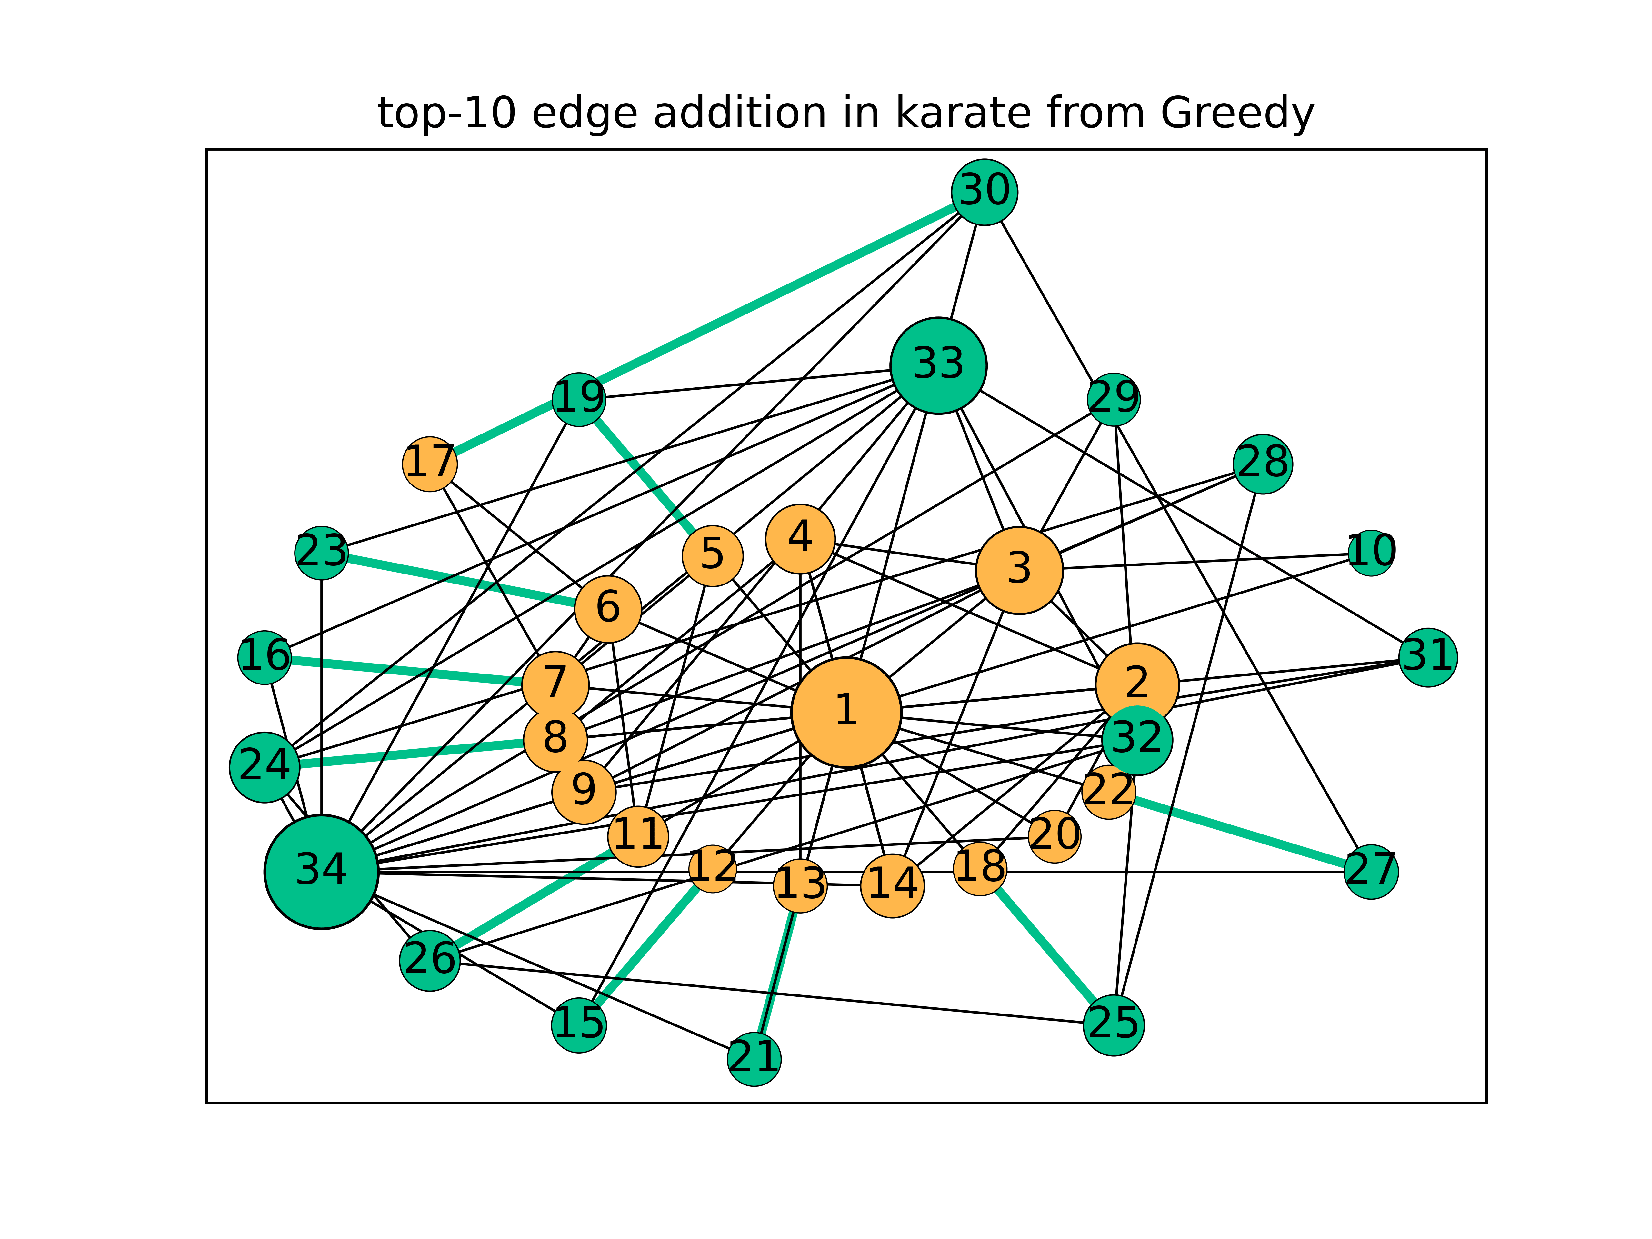
\includegraphics[width=0.65\textwidth]{Figures/top-10_karate_greedy}
	\caption{the top-10 edges proposed by the greedy algorithm}
	\label{fig:top-10-karate}
\end{figure}


\clearpage

\subsection{Heuristics in the Books dataset}

\begin{figure}[!htbp]
	\centering
	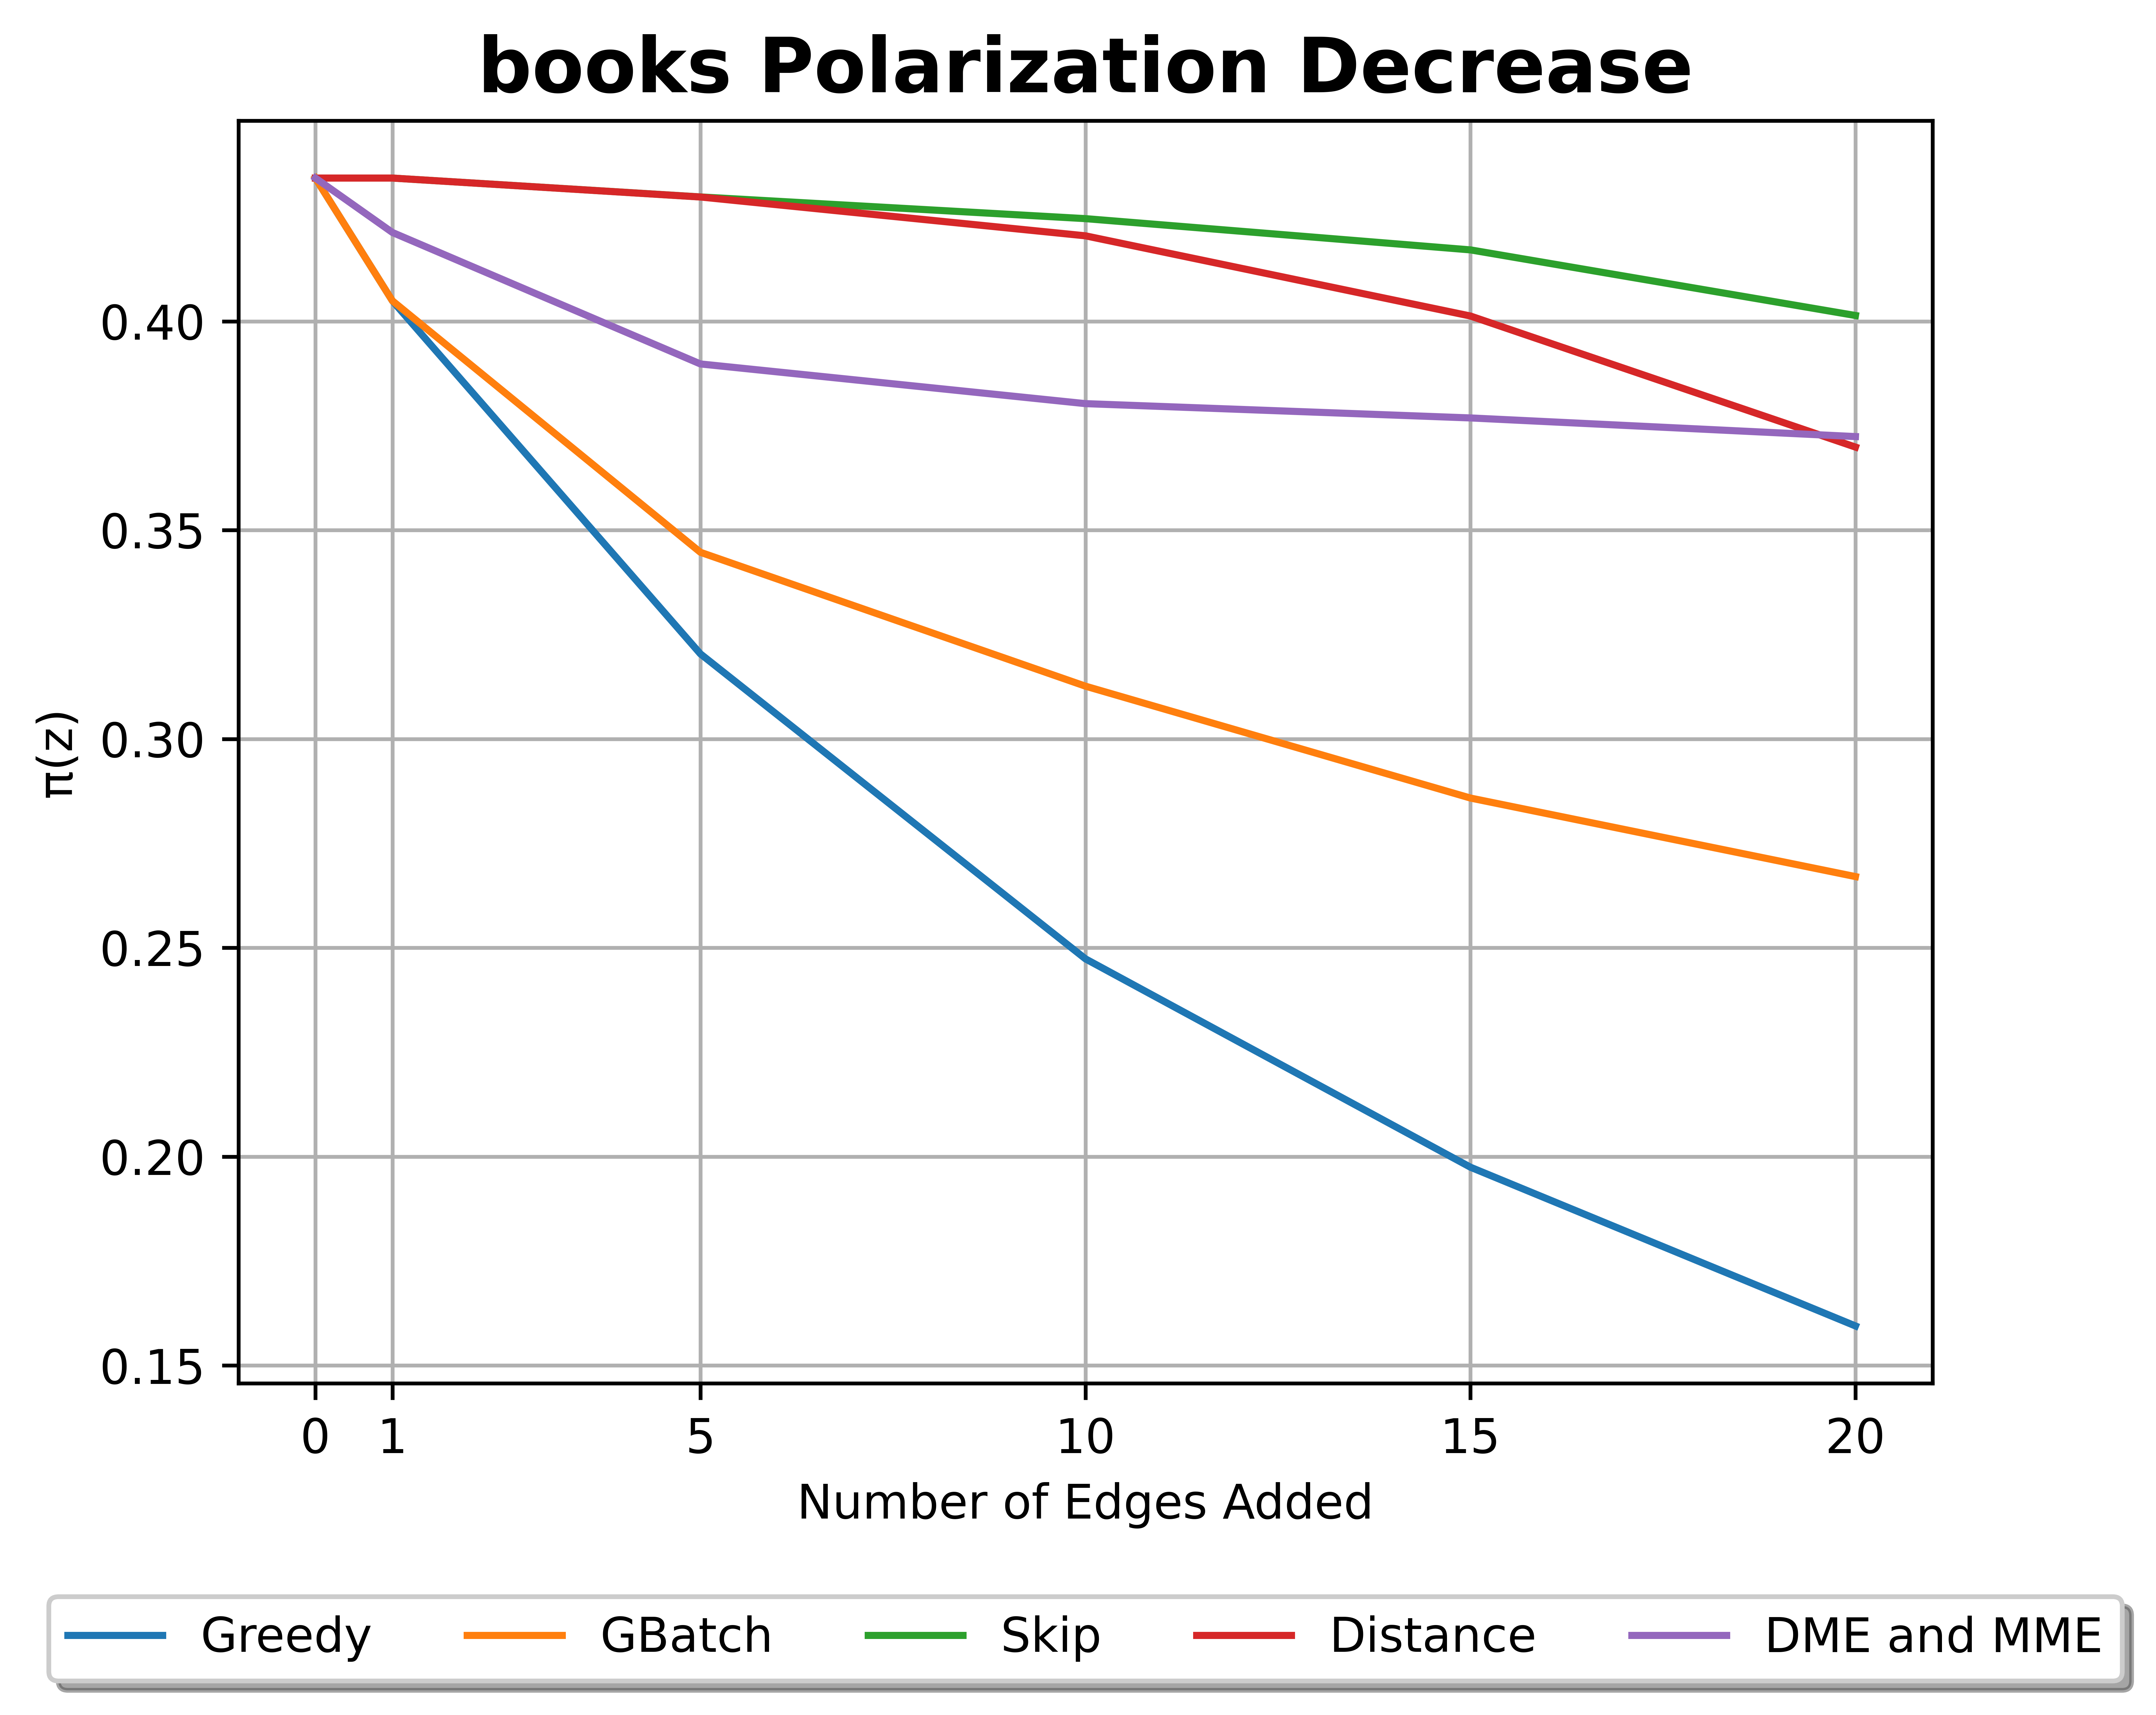
\includegraphics[width=0.65\textwidth]{Figures/books Polarization Decrease}
	\caption{Heuristic comparison of time in Books}
	\label{fig:books_pol}
\end{figure}


\begin{figure}[!htbp]
	\centering
	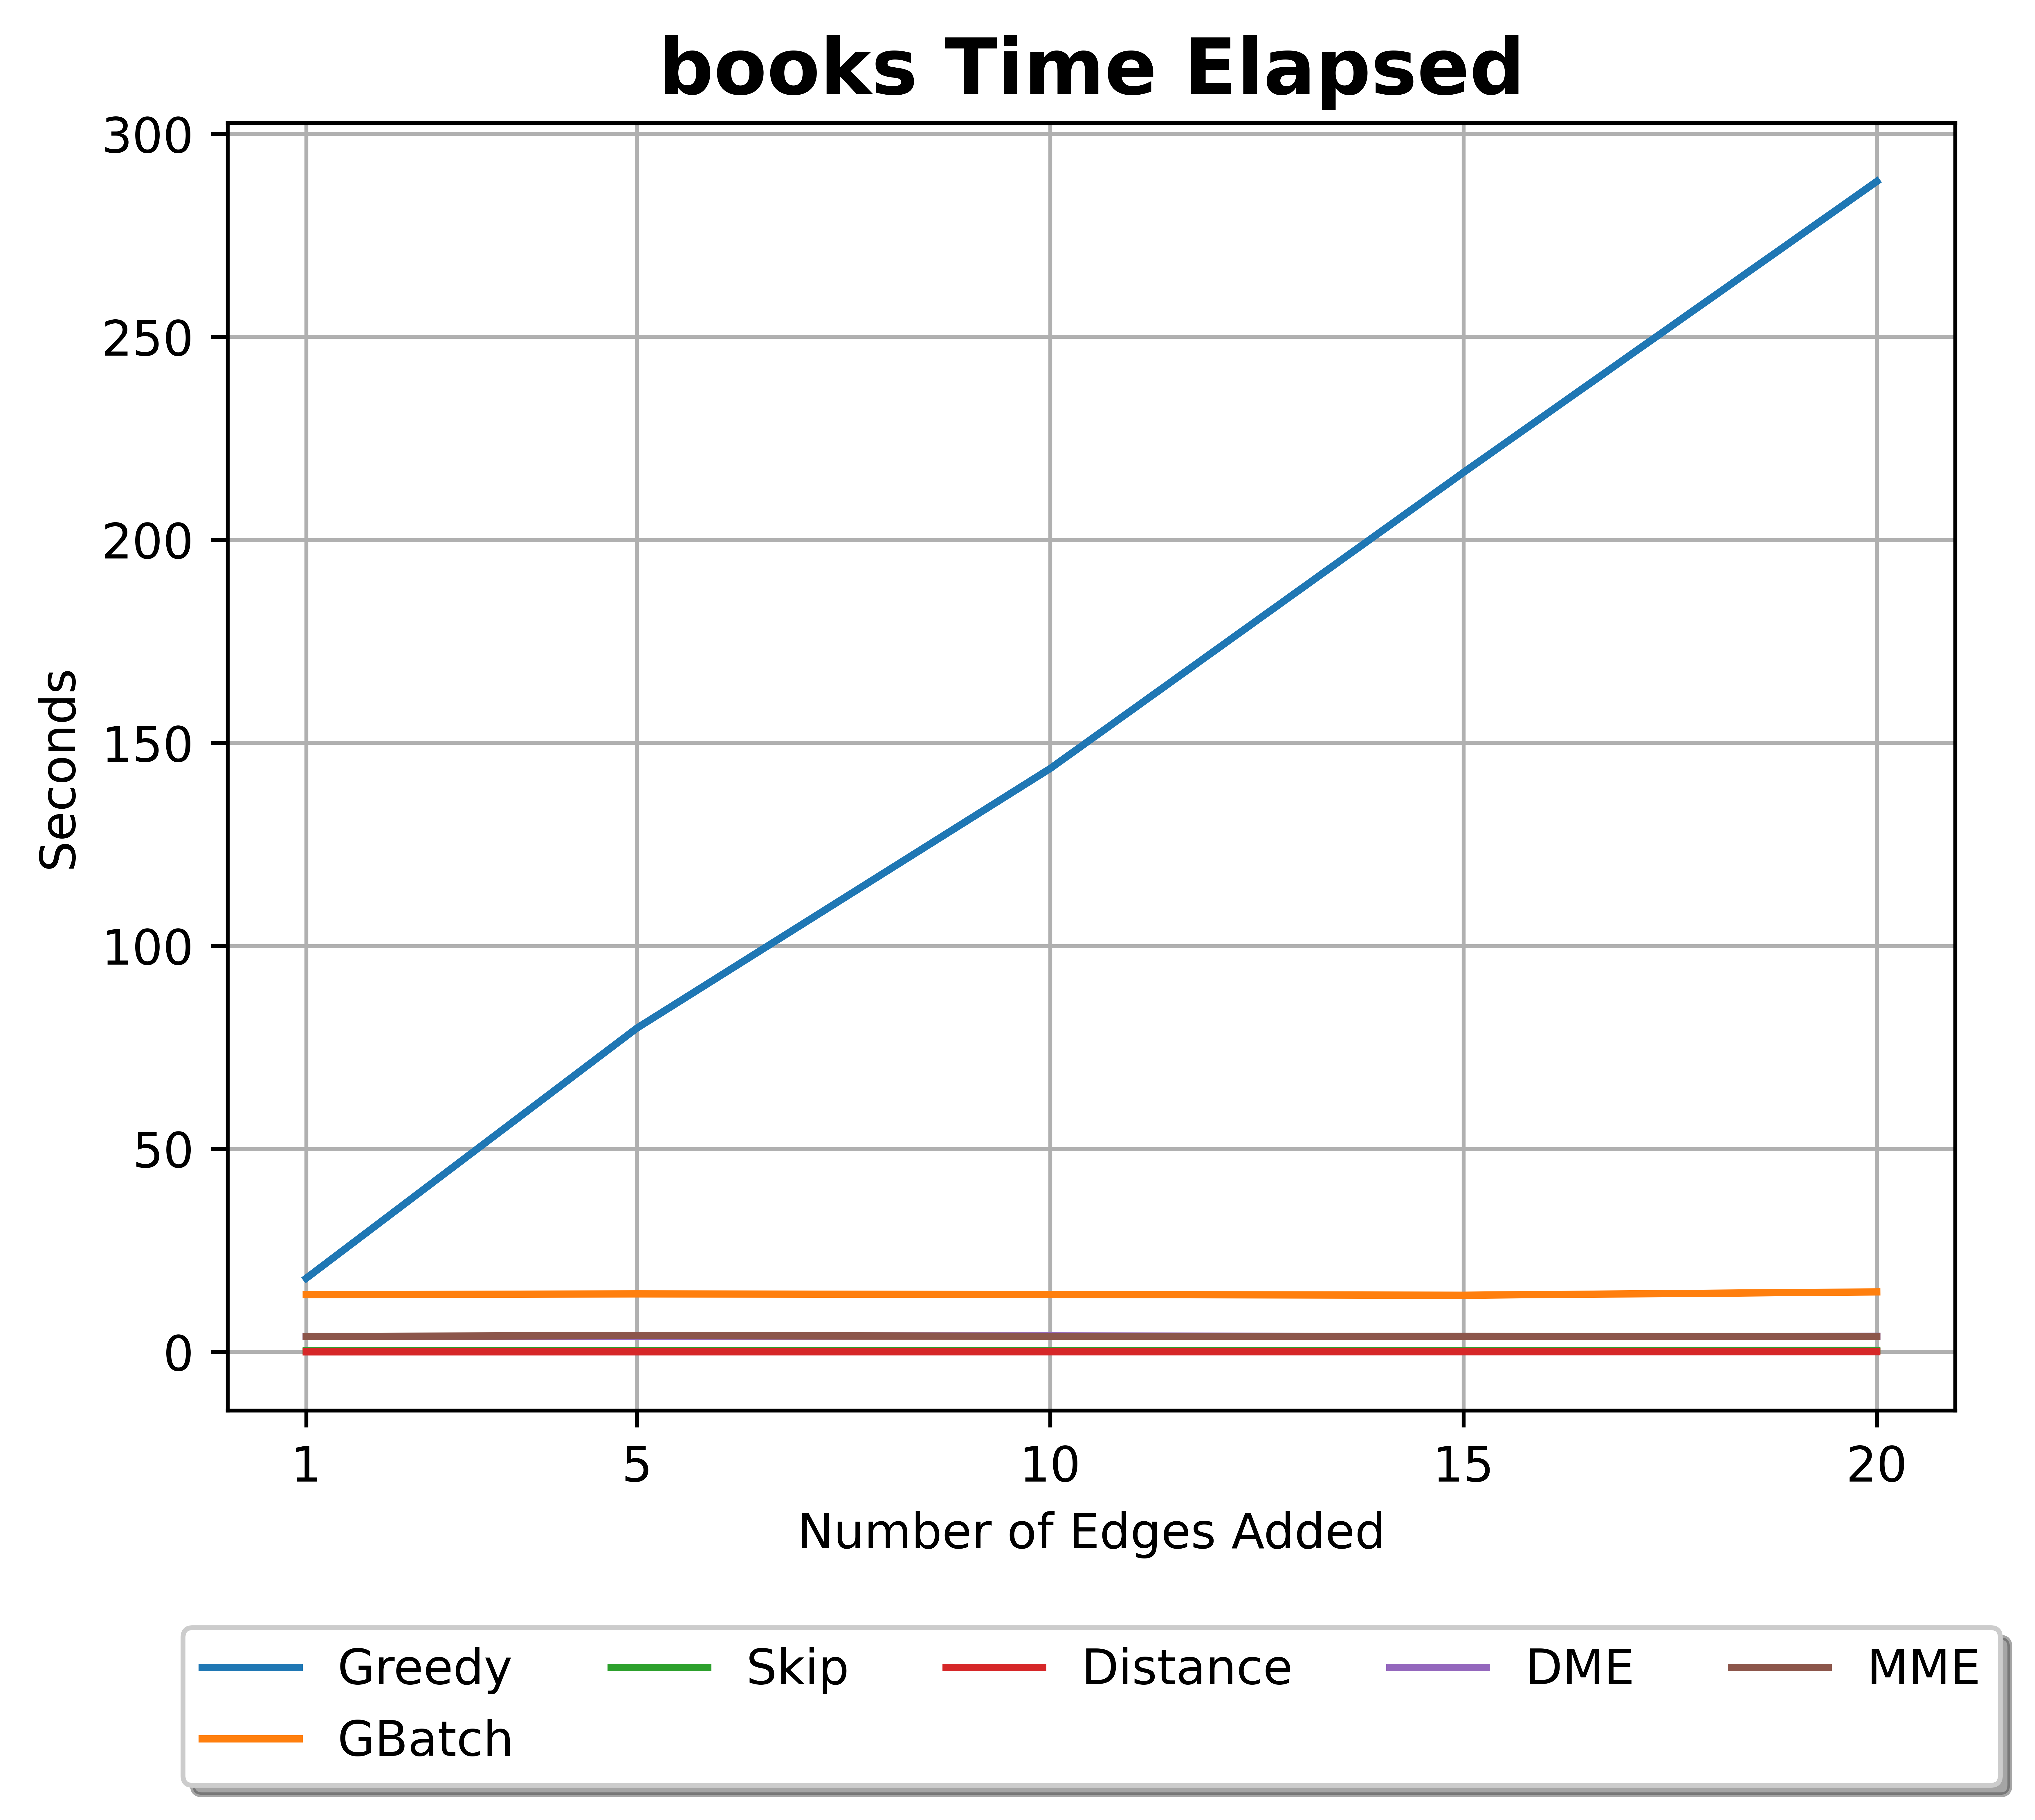
\includegraphics[width=0.65\textwidth]{Figures/books Time Elapsed}
	\caption{Heuristic comparison of time in Books}
	\label{fig:books_time}
\end{figure}


\clearpage


\subsection{Heuristics in the Beefban dataset}

\begin{figure}[!htbp]
	\centering
	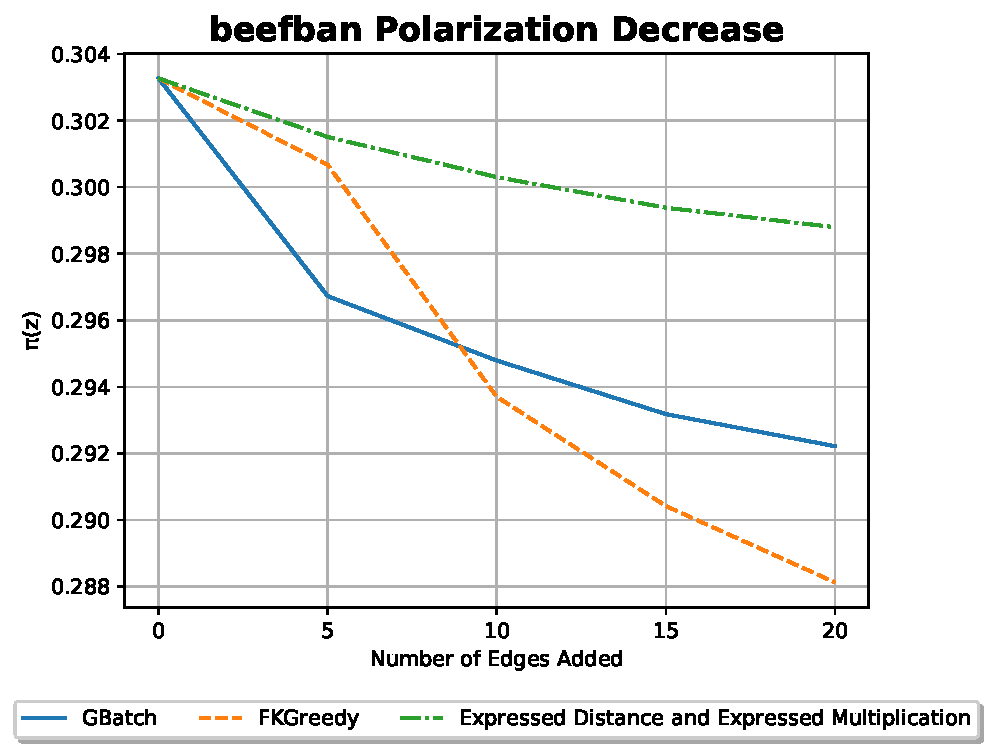
\includegraphics[width=0.65\textwidth]{Figures/beefban Polarization Decrease}
	\caption{Heuristic comparison of time in Beefban}
	\label{fig:beefban_pol}
\end{figure}


\begin{figure}[!htbp]
	\centering
	\includegraphics[width=0.65\textwidth]{Figures/Beefban Time Elapsed}
	\caption{Heuristic comparison of time in Beefban}
	\label{fig:beefban_time}
\end{figure}

\clearpage

\subsection{Heuristics in the Polblogs dataset}

\begin{figure}[!htbp]
	\centering
	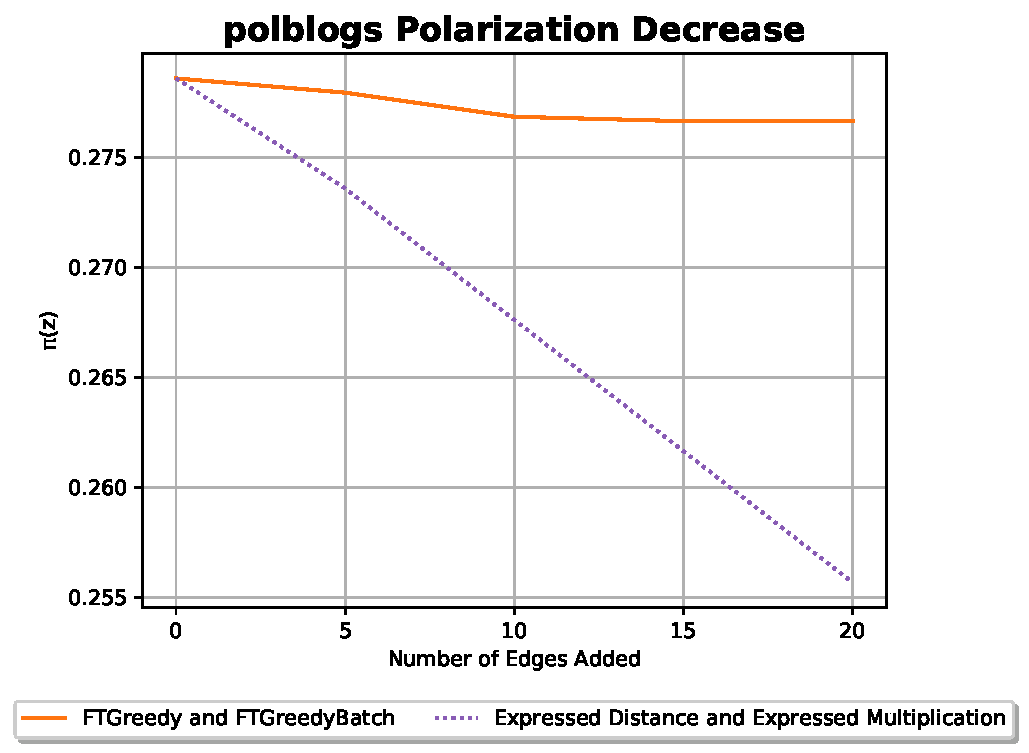
\includegraphics[width=0.65\textwidth]{Figures/polblogs Polarization Decrease}
	\caption{Heuristic comparison of time in Polblogs}
	\label{fig:polblogs_pol}
\end{figure}


\begin{figure}[!htbp]
	\centering
	\includegraphics[width=0.65\textwidth]{Figures/Polblogs Time Elapsed}
	\caption{Heuristic comparison of time in Polblogs}
	\label{fig:polblogs_time}
\end{figure}

\clearpage

\subsection{Heuristics in the GermanWings dataset}

\begin{figure}[!htbp]
	\centering
	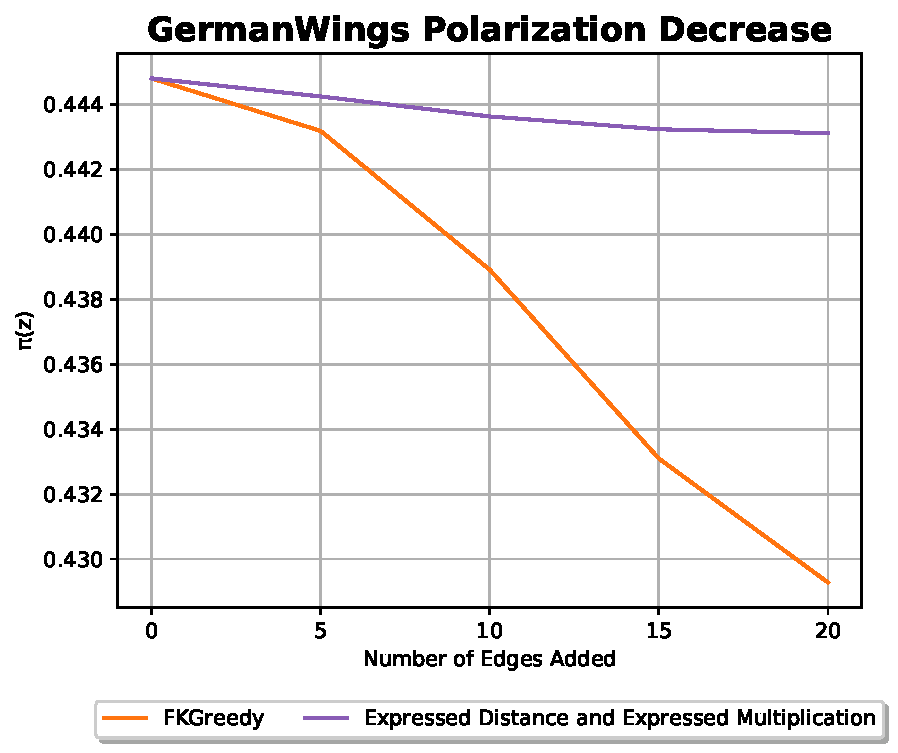
\includegraphics[width=0.65\textwidth]{Figures/GermanWings Polarization Decrease}
	\caption{Heuristic comparison of time in GermanWings}
	\label{fig:GermanWings_pol}
\end{figure}


\begin{figure}[!htbp]
	\centering
	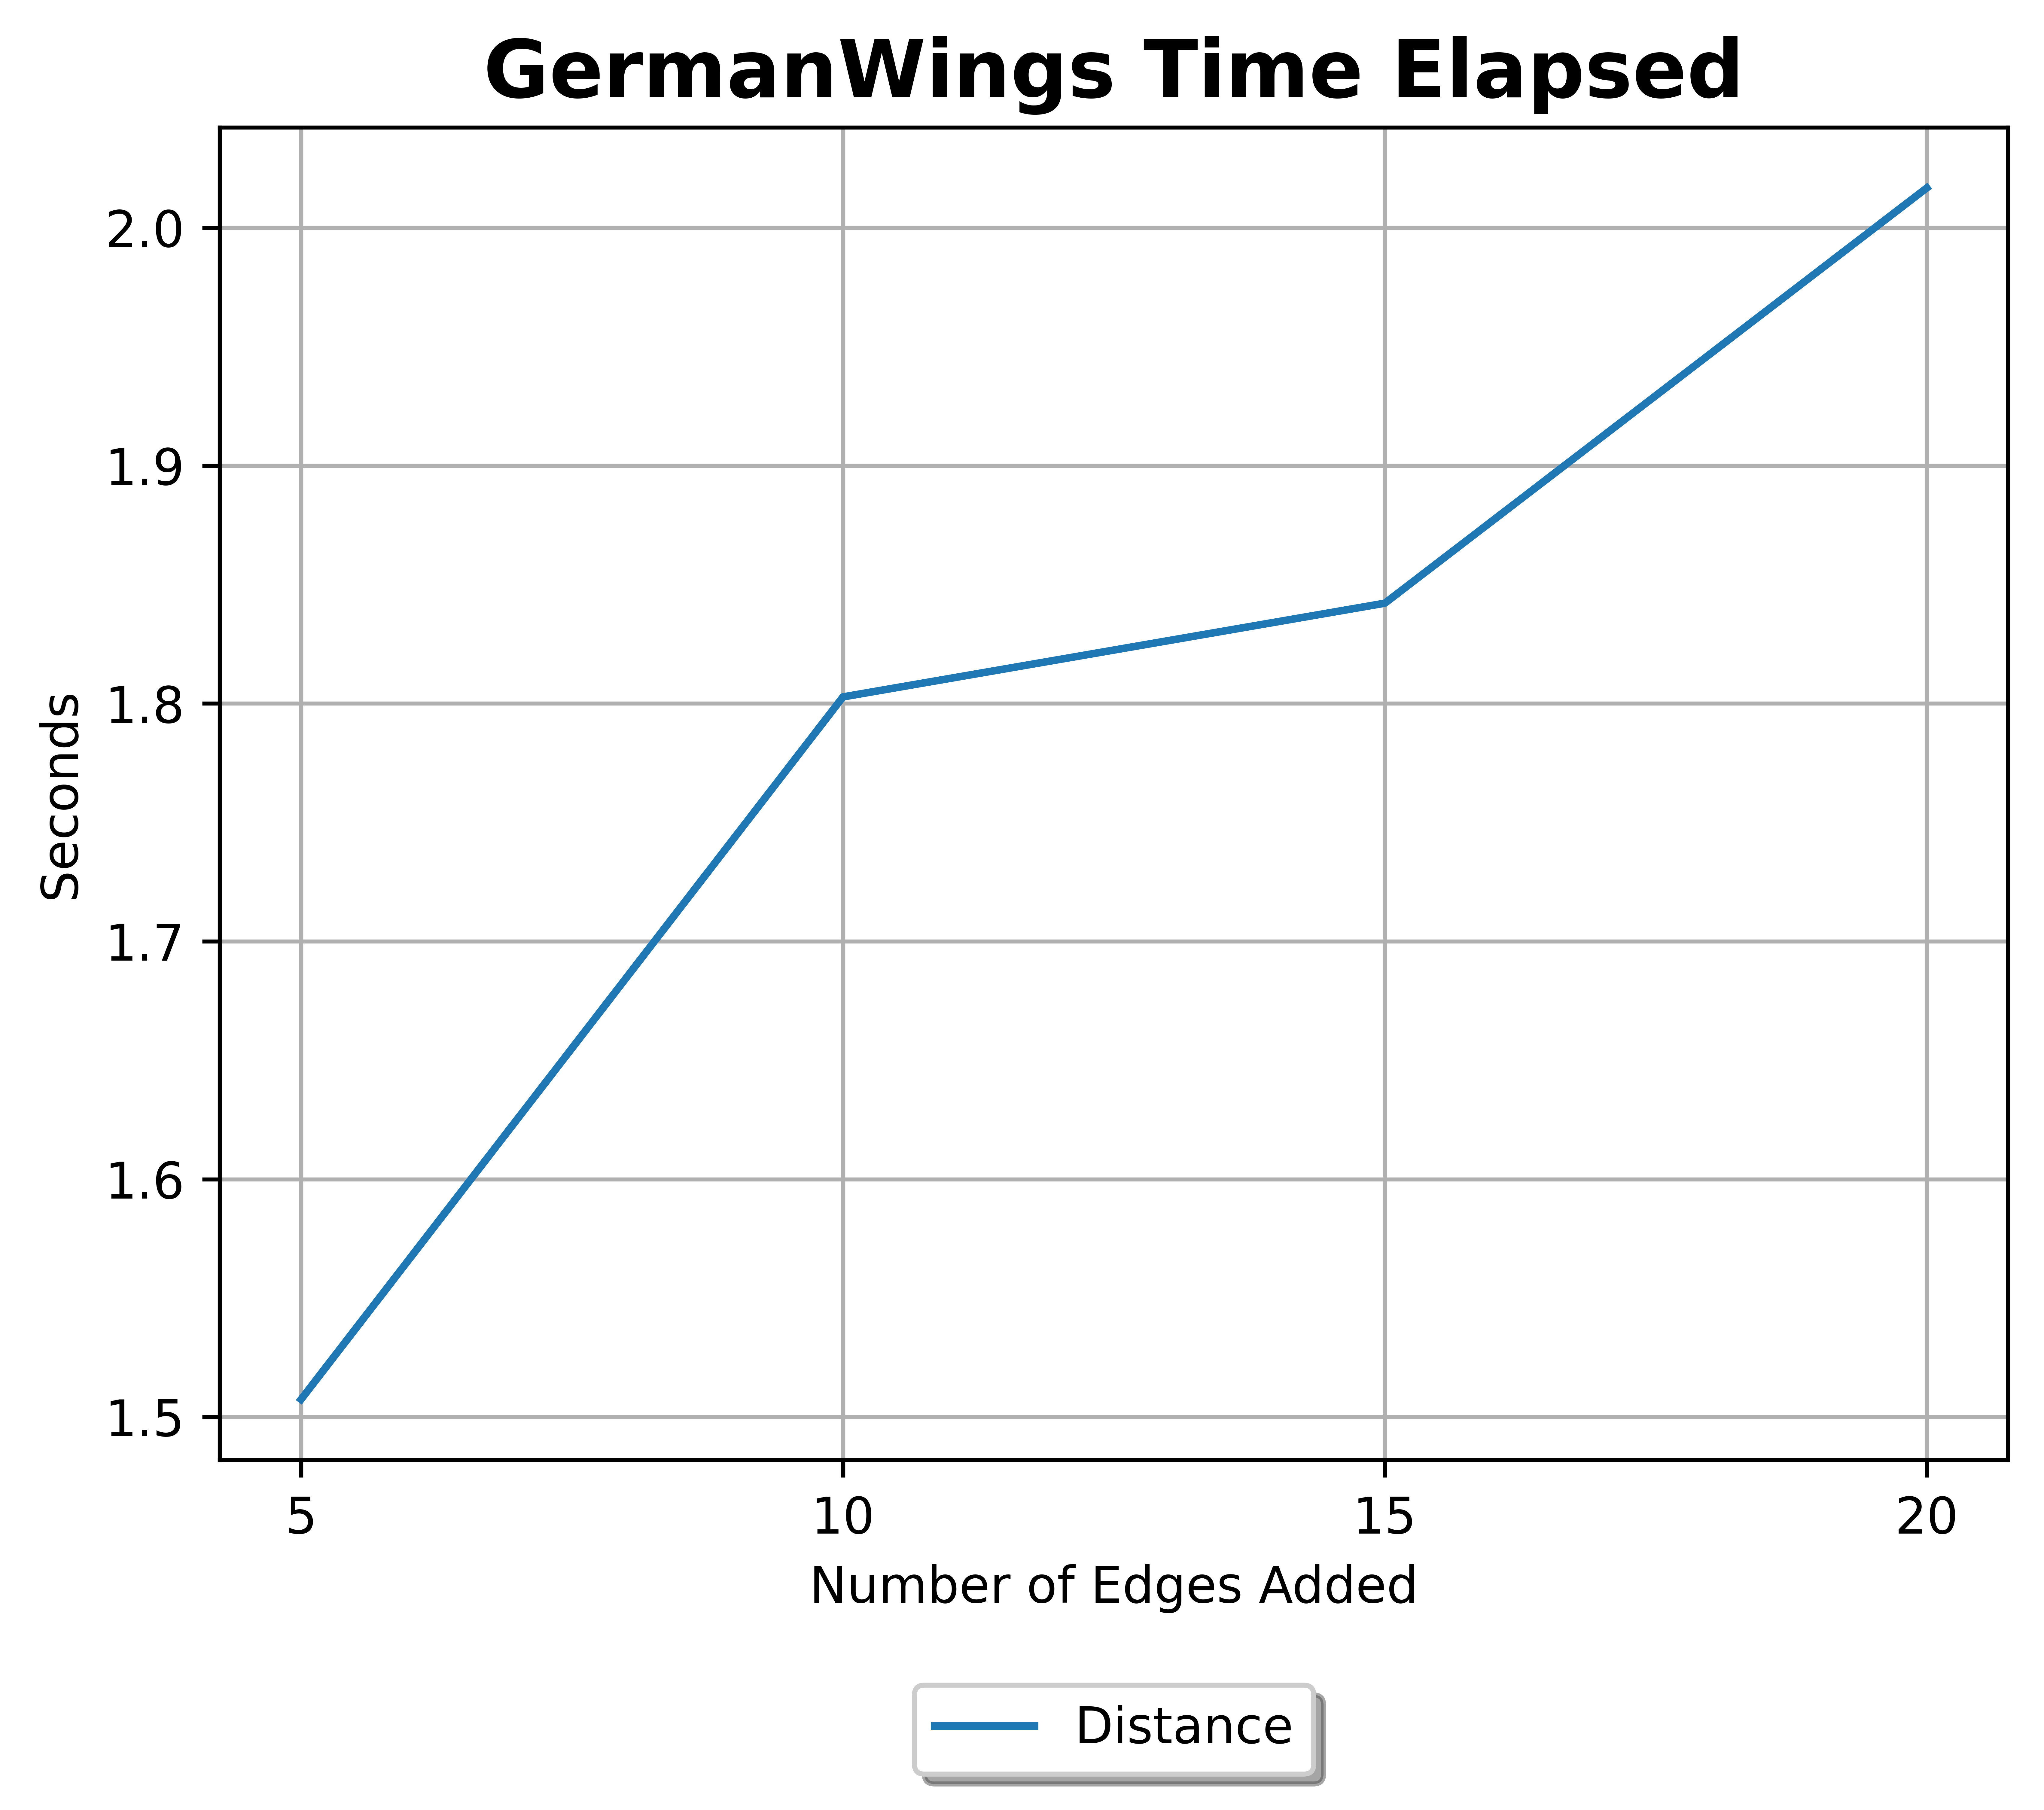
\includegraphics[width=0.65\textwidth]{Figures/GermanWings Time Elapsed}
	\caption{Heuristic comparison of time in GermanWings}
	\label{fig:GermanWings_time}
\end{figure}
\clearpage


\subsection{Heuristics in the ClintonTrump dataset}
\begin{figure}[!htbp]
	\centering
	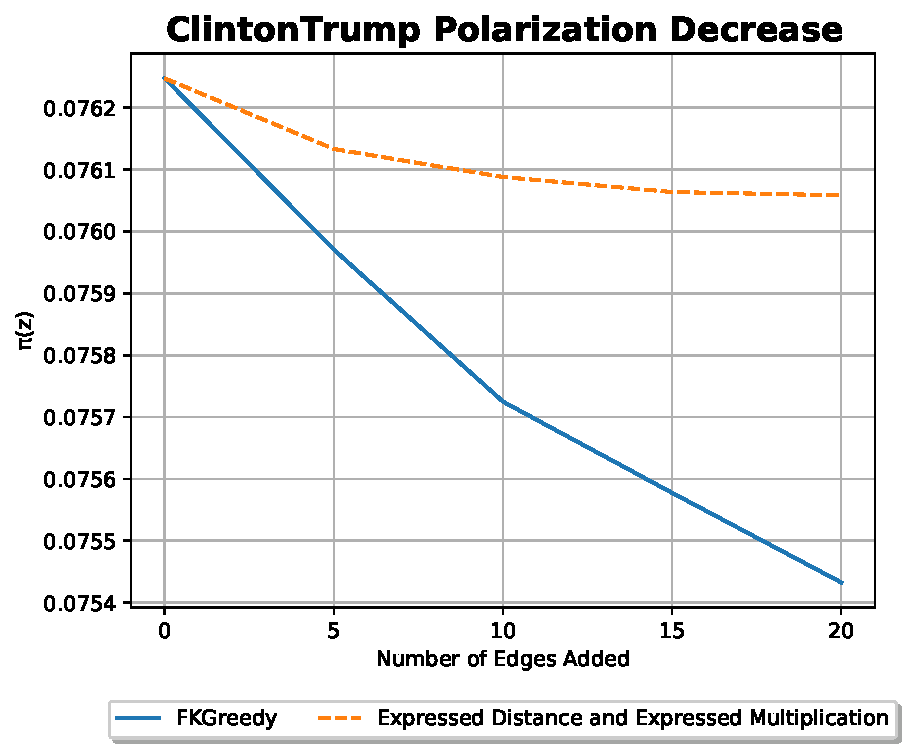
\includegraphics[width=0.65\textwidth]{Figures/ClintonTrump Polarization Decrease}
	\caption{Heuristic comparison of time in ClintonTrump}
	\label{fig:ClintonTrump_pol}
\end{figure}


\begin{figure}[!htbp]
	\centering
	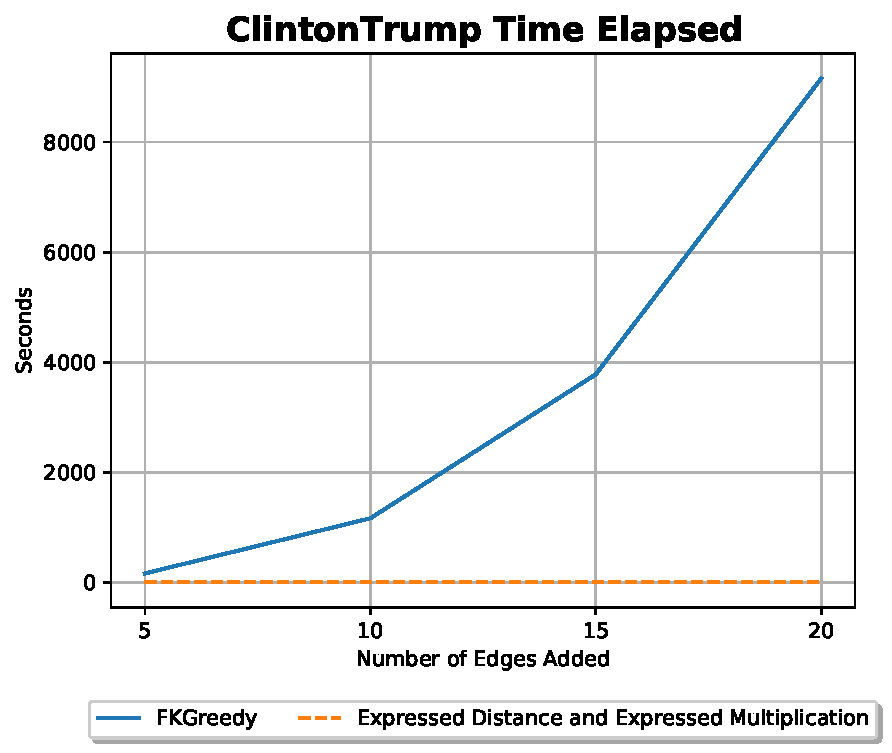
\includegraphics[width=0.65\textwidth]{Figures/ClintonTrump Time Elapsed}
	\caption{Heuristic comparison of time in ClintonTrump}
	\label{fig:ClintonTrump_time}
\end{figure}
\clearpage


\subsection{Heuristics in the SXSW dataset}



\clearpage


\section{Polarization decrease by removing edges}
\label{sec:polremovingdecrease}
Bellow we examine the removal of edges from a social graph and their result in polarization. We also find the edge betweenness centrality of each edge. 
\\
\\
The edge betweenness centrality is defined as the number of the shortest paths that go through an edge in a graph or network.(add cite Girvan and Newman 2002). 
\\
\\
In the tables following, Sign and Addition refer to the multiplication and the addition of the opinions of the nodes that are attached to the specific edge examined. Graphs in the books and blogs datasets, due to size, are omitted.
\\
\\

\subsection{Edges removal in the Karate dataset}

\begin{table}[H]
 \centering
 \caption{Edges with the biggest increase of polarization}
 \label{tab:edgesLargest}
 \begin{tabular}{| l || l | l | l | l |}
 \hline
  Edge & Betweenness Centrality & Polarization Increase & Sign & Addition\\
  \hline
  \hline
  (1, 32) & $0.12725$ & $0.04669$ & - &  0\\
  \hline
  (20, 34) & $0.059384$ & $0.03470$ & - &  0\\
  \hline
  (14, 34) & $0.06782$ & $0.02924$ & - &  0\\
  \hline
  (2, 31) & $0.03228$ & $0.02505$ & - &  0\\
  \hline
  (3, 28) & $0.04119$ & $0.02068$ & - &  0\\
  \hline
 \end{tabular}
  
 \caption{Edges with the biggest decrease of polarization }
 \label{tab:edgesLargest}
 \begin{tabular}{| l || l | l | l | l |}
 \hline
  Edge & Betweenness Centrality & Polarization Decrease & Sign & Addition\\
  \hline
  \hline
  (5, 11) & $0.00297$ & $5.55111*10^{-17}$ & + &  -2\\
  \hline
  (4, 8) & $0.00336$ & $3.04869*10^{-7}$ & + &  -2\\
  \hline
  (1, 4) & $0.02049$ & $1.38023*10^{-5}$ & + &  -2\\
  \hline
  (32, 34) & $0.05339$ & $1.61826*10^{-5}$ & + &  +2\\
  \hline
  (1, 8) & $0.02282$ & $1.93446*10^{-5}$ & + &  -2\\
  \hline
  \hline
 \end{tabular}
\end{table}

\begin{figure}[H]
	\centering
	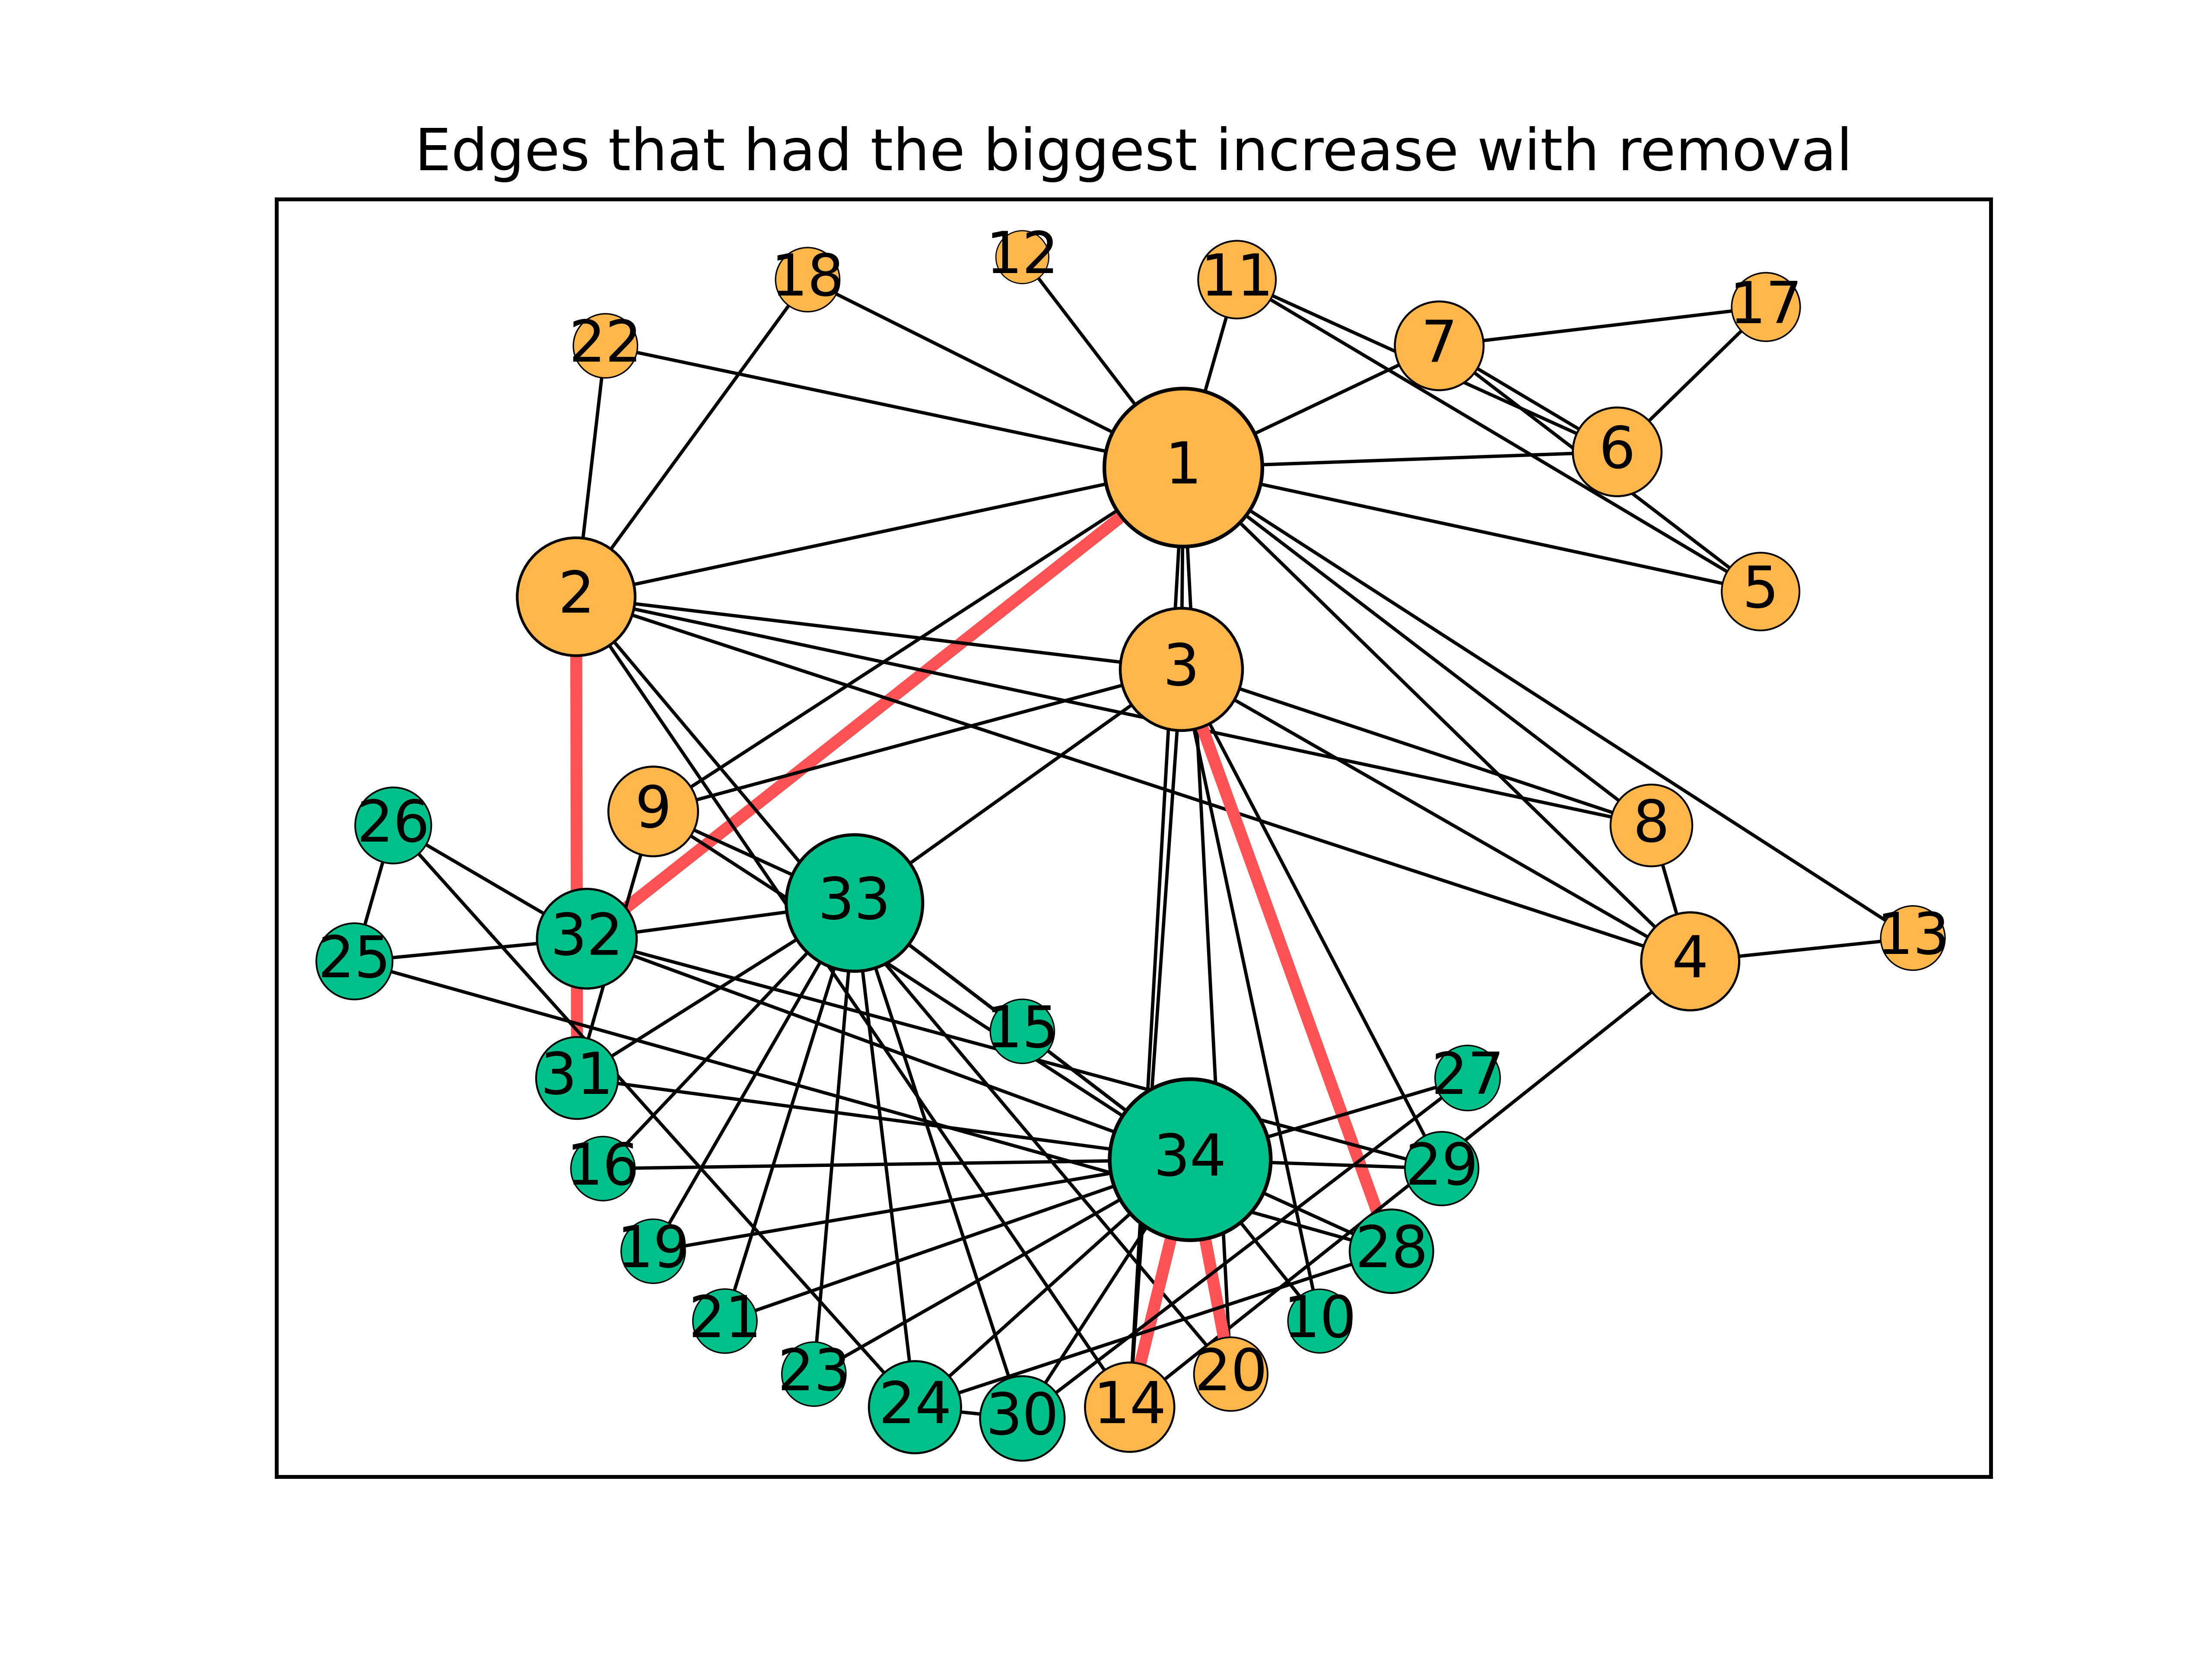
\includegraphics[width=0.65\textwidth]{Figures/karate_increase}
	\label{fig:karate_increase}
	\caption{Removing edges in Karate}
\end{figure}

\begin{figure}[H]
	\centering
	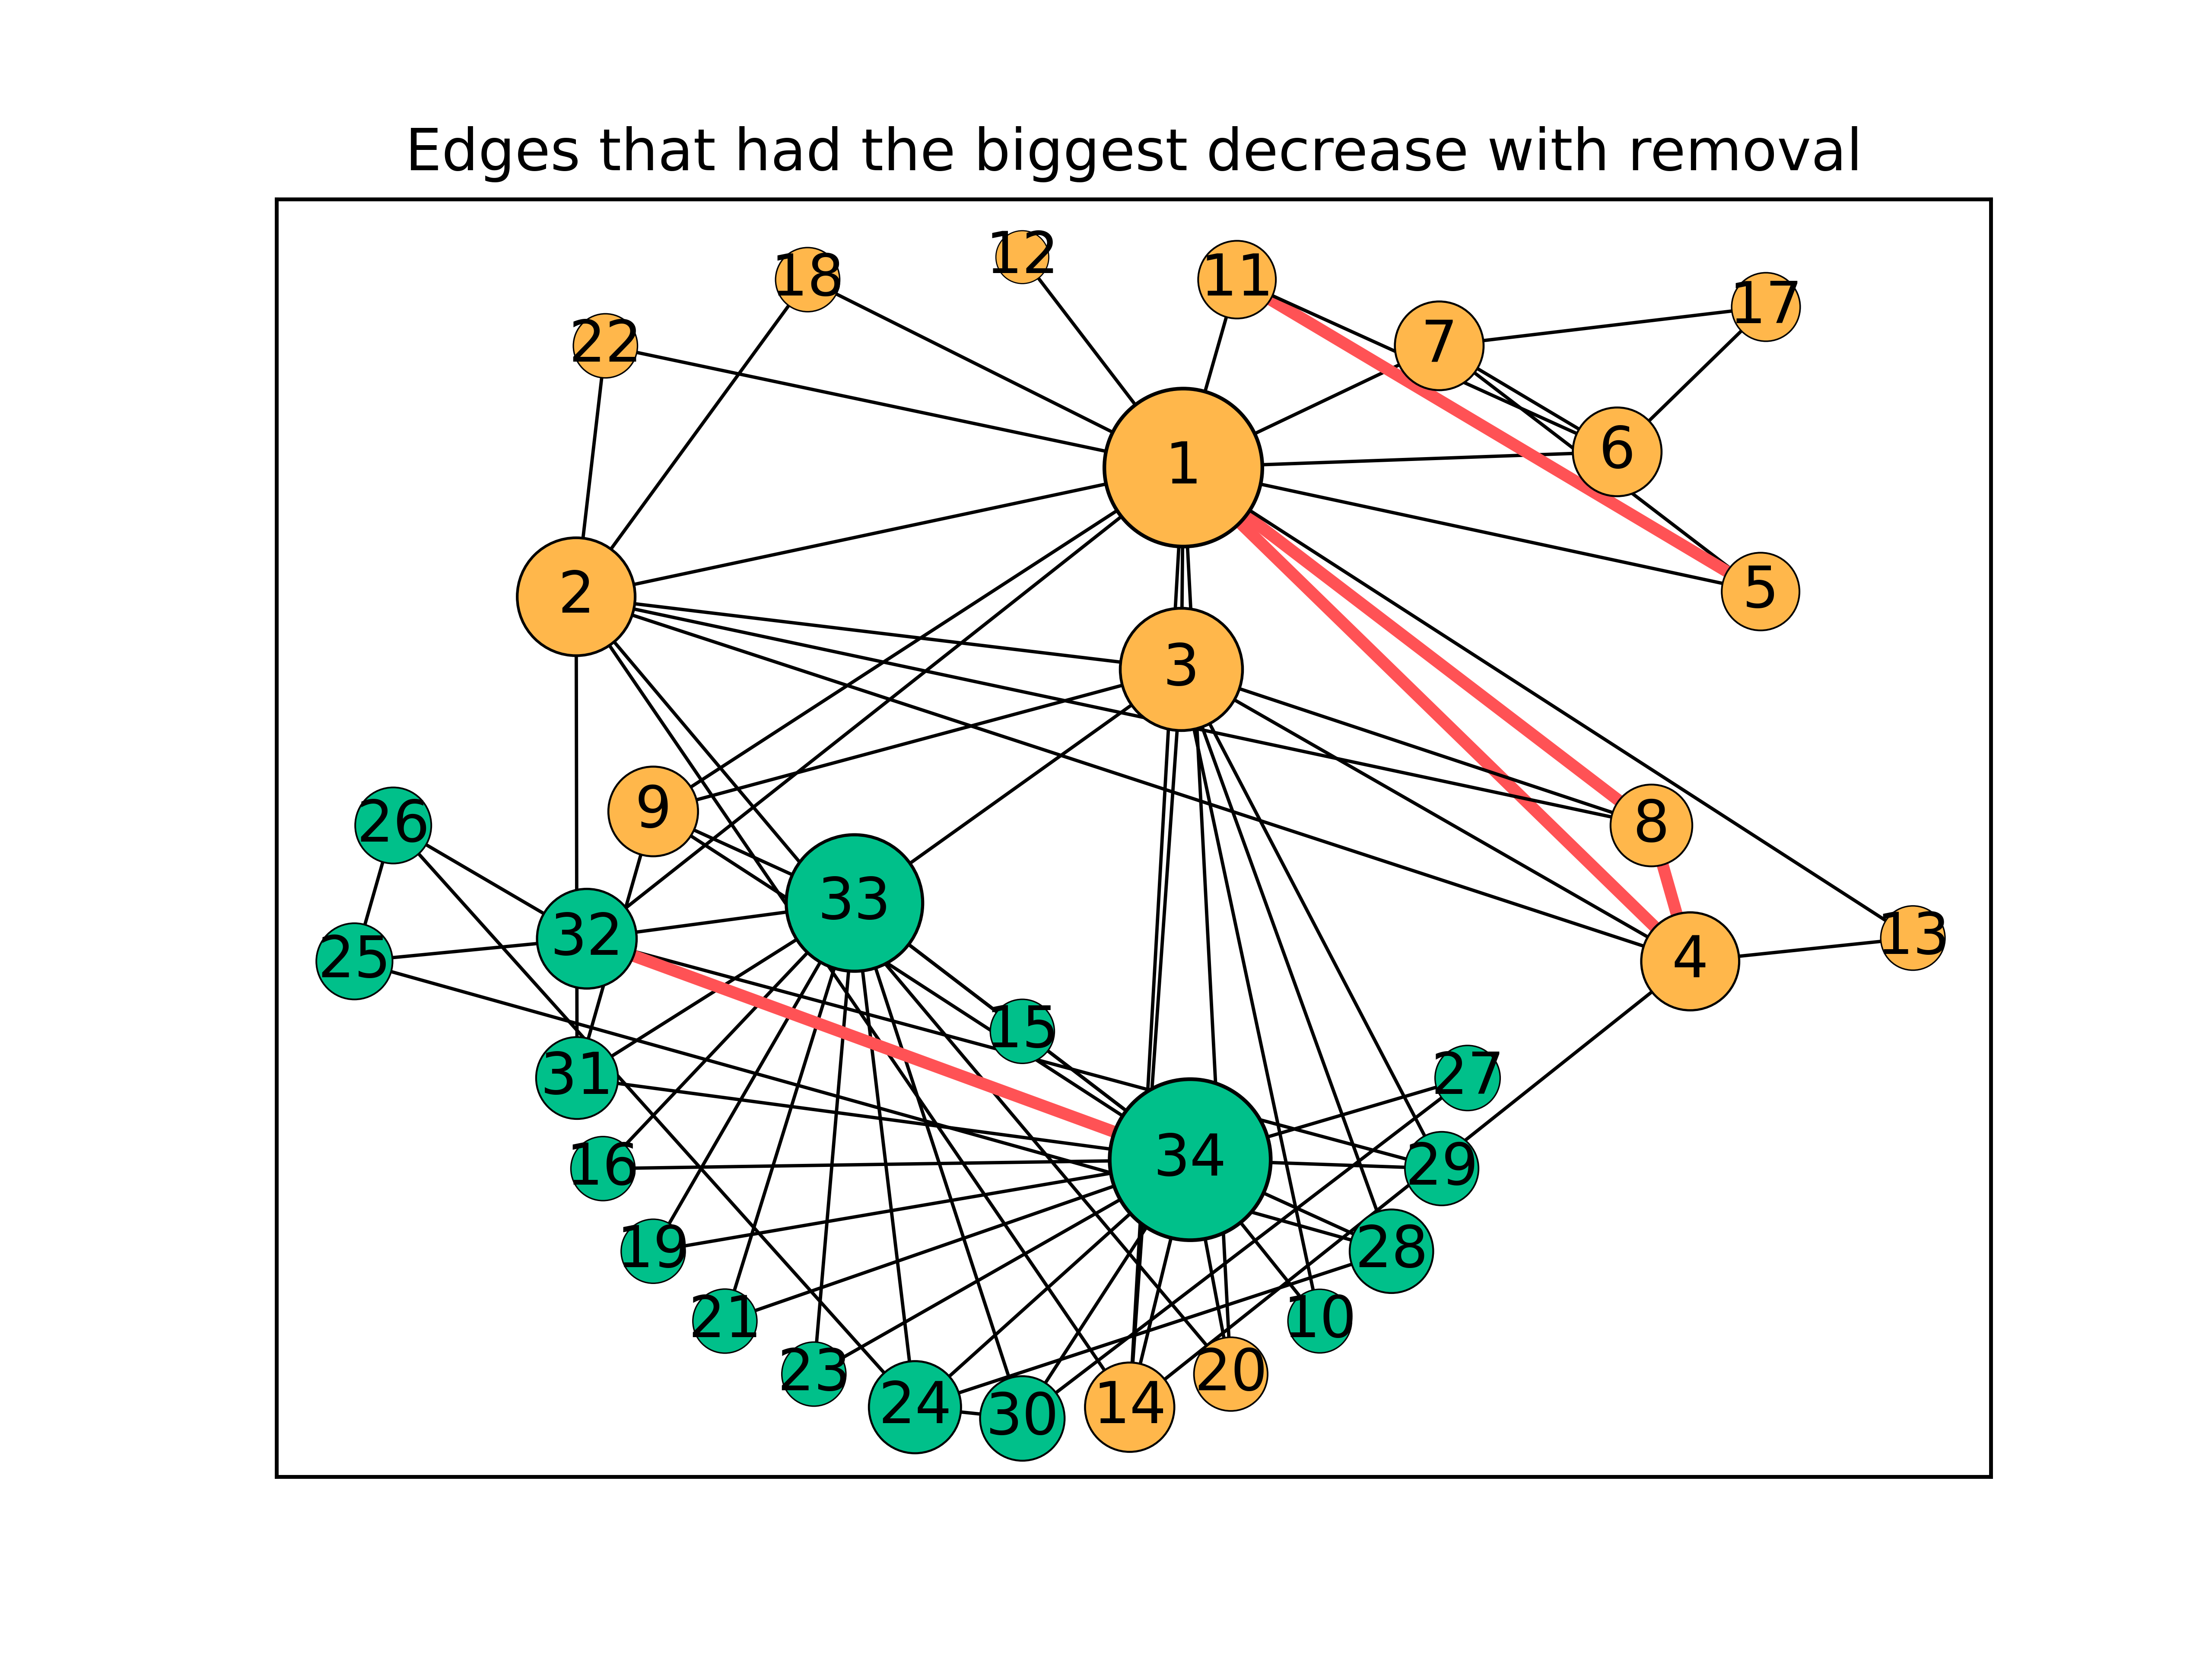
\includegraphics[width=0.65\textwidth]{Figures/karate_decrease}
	\label{fig:karate_decrease}
	\caption{Removing edges in Karate}
\end{figure}


\subsection{Edges removal in the Blogs dataset}

\begin{table}[H]
 \centering
 \caption{Edges with the biggest increase of polarization}
 \label{tab:edgesLargest}
 \begin{tabular}{| l || l | l | l | l |}
 \hline
  Edge & Betweenness Centrality & Polarization Increase & Sign & Addition\\
  \hline
  \hline
  (213, 793) & $0.00219$ & $0.00091$ & - &  0\\
  \hline
  (600, 1183) & $0.00439$ & $0.00074$ & - &  0\\
  \hline
  (523, 1375) & $0.00110$ & $0.00070$ & - &  0\\
  \hline
  (325, 1159) & $0.00110$ & $0.00069$ & - &  0\\
  \hline
  (632, 1000) & $0.00110$ & $0.00069$ & - &  0\\
  \hline
 \end{tabular}
 
 
 \caption{Edges with the biggest decrease of polarization }
 \label{tab:edgesLargest}
 \begin{tabular}{| l || l | l | l | l |}
 \hline
  Edge & Betweenness Centrality & Polarization Decrease & Sign & Addition\\
  \hline
  \hline
  (574, 1380) & $0.00014$ & $2.09620*10^{-6}$ & - &  0\\
  \hline
  (23, 1380) & $0.00021$ & $2.18102*10^{-6}$ & - &  0\\
  \hline
  (600, 1021) & $0.00024$ & $2.41460*10^{-6}$ & - &  0\\
  \hline
  (634, 1380) & $0.00010$ & $2.60119*10^{-6}$ & - &  0\\
  \hline
  (219, 1380) & $0.00014$ & $2.91467*10^{-6}$ & - &  0\\
  \hline
  \hline
 \end{tabular}
 
\end{table}

\subsection{Edges removal in the Books dataset}
\begin{table}[H]
 \centering
 \caption{Edges with the biggest increase of polarization }
 \label{tab:edgesLargest}
 \begin{tabular}{| l || l | l | l | l |}
 \hline
  Edge & Betweenness Centrality & Polarization Increase & Sign & Addition\\
  \hline
  \hline
  (0, 5) & $0.00056$ & $2.65885*10^5$ & - &  0\\
  \hline
  (7, 58) & $0.00713$ & $0.00012$ & - &  0\\
  \hline
  (5, 6) & $0.00222$ & $0.00012$ & - &  0\\
  \hline
  (6, 18) & $0.00858$ & $0.00014$ & +& -2\\
  \hline
  (0, 2) & $0.00031$ & $0.00349$ & - &  0\\
  \hline
 \end{tabular}
\end{table}

\begin{table}[H]
 \centering
 \caption{Edges with the biggest decrease of polarization}
 \label{tab:edgesLargest}
 \begin{tabular}{| l || l | l | l | l |}
 \hline
  Edge & Betweenness Centrality & Polarization Decrease & Sign & Addition\\
  \hline
  \hline
  (53, 76) & $0.06290$ & $0.01985$ & - &  0\\
  \hline
  (46, 102) & $0.04914$ & $0.01541$ & + &  -2\\
  \hline
  (19, 77) & $0.04367$ & $0.01458$ & + &  +2\\
  \hline
  (9, 51) & $0.02812$ & $0.01000$ & - &  0\\
  \hline
  (49, 72) & $0.06809$ & $0.00952$ & - &  0\\
  \hline
 \end{tabular} 
\end{table}

\subsection{Remarks about the edge removals}

We can clearly see that there is an association between the edge betweenness centrality and the decrease in polarization. Edges that contribute to a bigger decrease have larger betweenness centrality. 
\\
\\
A second thing that we see in all three datasets is that the biggest increase is coming from the removal of edges that connect opposing opinions.
\\
\\
In addition, during the experiments on the karate dataset, the removal of edge $(6, 7)$ had no effect on the polarization index. This leads to the following lemma.

\begin{lemma}
The polarization index can stay the same after an edge removal.
\end{lemma}




% Εισαγωγή της βιβλιογραφίας
\addstarredchapterc{\bibname} % minitoc
\bibliographystyle{IEEEtran}
\bibliography{/Users/leonidas/Desktop/February 21/thesis/LaTeXthesis/Template/Content/Bibliography}

% Προαιρετικά, μπορείτε να εισάγετε παραρτήματα
%\appendix 
%\chapter{Τίτλος πρώτου παραρτήματος}
\label{app:FirstAppendix}

Εδώ είναι ο χώρος του πρώτου Παραρτήματος.

\begin{table}[h]
	\centering
	\caption{Πίνακας Παραρτήματος.}
	\label{tab:AppendixTable}
	\begin{tabular}{l l l l l}
		\hline
		~ & ~ & Sample Mean & ~ & 95\% Confidence Interval \\
		\hline
		1 process & ~ & $3.640966$  & ~ & $0.100136$ \\
		4 processes & ~ & $1.053655$  & ~ & $0.037212$ \\
		8 processes & ~ & $0.610223$  & ~ & $0.023470$ \\
		16 processes & ~ & $0.357321$  & ~ & $0.014783$ \\
		32 processes & ~ & $0.227180$  & ~ & $0.016923$ \\
		\hline
	\end{tabular}
\end{table}
%\chapter{Τίτλος δεύτερου παραρτήματος}
\label{app:SecondAppendix}

\section{Τίτλος πρώτης ενότητας}
\label{sec:FirstSection}
Εδώ είναι ο χώρος της πρώτης ενότητας του δεύτερου Παραρτήματος.

\section{Τίτλος δεύτερης ενότητας}
\label{sec:SecondSection}
Εδώ είναι ο χώρος της δεύτερης ενότητας του δεύτερου Παραρτήματος.
%\chapter{Τίτλος τρίτου παραρτήματος}
\label{app:ThirdAppendix}

Εδώ είναι ο χώρος του τρίτου Παραρτήματος.

\begin{figure}[h]
	\centering
	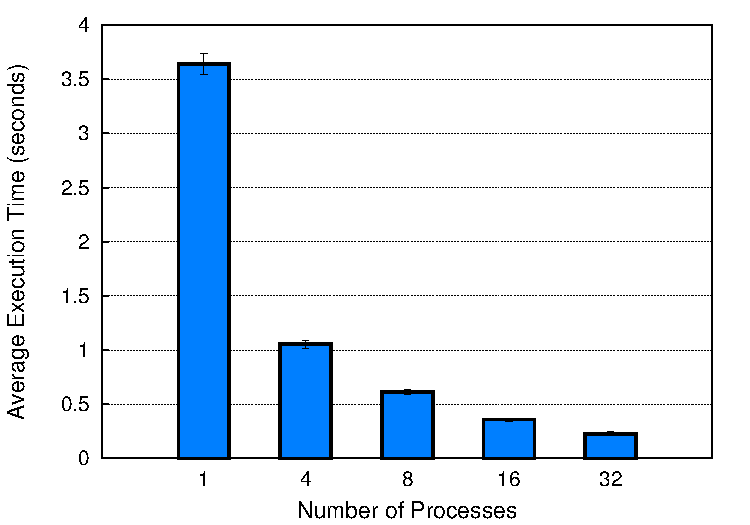
\includegraphics[width=0.65\textwidth]{Figures/MatrixMultiplication.pdf}
	\caption{Εικόνα Παραρτήματος.}
	\label{fig:AppendixFigure}
\end{figure}


% Εκτύπωση του ευρετηρίου (προαιρετικό)
%\printindex


% Σελίδες χωρίς αρίθμηση
\pagenumbering{gobble}

%\pdfbookmark[0]{\csedimosieuseis}{dimosieuseis} % hyperref
\chapter*{\csedimosieuseis}

Προαιρετικά, βάζουμε μία λίστα με τις δημοσιεύσεις του συγγραφέα. % Προαιρετικό

% Σύντομο Βιογραφικό
%\pdfbookmark[0]{\cseviografiko}{viografiko} % hyperref
\chapter*{\cseviografiko}

Ένα σύντομο βιογραφικό είναι απαραίτητο.

\end{document}




Κάθε καταχώρηση ξεκινά με τη δήλωση του τύπου της αναφοράς.
Το παραπάνω παράδειγμα αποτελεί αναφορά σε ένα άρθρο περιοδικού, επομένως η καταχώρηση ξεκινά με τη δήλωση \verb|@article|.
Στη συνέχεια αναθέτουμε ένα μοναδικό κλειδί στην καταχώρηση, π.χ. \verb|Newman2003a|, το οποίο χρησιμοποιούμε στο κείμενο της διατριβής για να αναφερθούμε σε αυτή με την εντολή \verb|\cite{Newman2003a}|.
Τέλος, συμπληρώνουμε τα πεδία του αντίστοιχου τύπου αναφοράς, μερικά από τα οποία είναι υποχρεωτικά.
Για παράδειγμα, στις καταχωρήσεις άρθρων είναι υποχρεωτική η συμπλήρωση των πεδίων \verb|author|, \verb|title|, \verb|journal|, και \verb|year|.

Η βιβλιογραφία της διατριβής στοιχειοθετείται αυτόματα μετά το τέλος των κεφαλαίων, με κάθε καταχώρηση να έχει έναν χαρακτηριστικό αριθμό.
Ο χαρακτηριστικός αριθμός της κάθε καταχώρησης εμφανίζεται μεταξύ αγκυλών στα σημεία του κειμένου της διατριβής όπου αναφερθήκαμε σε αυτή την καταχώρηση.
Για παράδειγμα, σε αυτήν την πρόταση αναφερόμαστε σε ένα άρθρο περιοδικού~\cite{Newman2003a}, σε μία εργασία συνεδρίου~\cite{DeCandia2007a}, σε μία τεχνική αναφορά~\cite{Jain1984a}, και σε ένα βιβλίο~\cite{Golumbic2004a}.










\section{Polarization decrease by removing edges}
\label{sec:polremovingdecrease}
Bellow we examine the removal of edges from a social graph and their result in polarization. We also find the edge betweenness centrality of each edge. 
\\
\\
The edge betweenness centrality is defined as the number of the shortest paths that go through an edge in a graph or network.(add cite Girvan and Newman 2002). 
\\
\\
In the tables following, Sign and Addition refer to the multiplication and the addition of the opinions of the nodes that are attached to the specific edge examined. Graphs in the books and blogs datasets, due to size, are omitted.
\\
\\

\subsection{Edges removal in the Karate dataset}

\begin{table}[H]
 \centering
 \caption{Edges with the biggest increase of polarization}
 \label{tab:edgesLargest}
 \begin{tabular}{| l || l | l | l | l |}
 \hline
  Edge & Betweenness Centrality & Polarization Increase & Sign & Addition\\
  \hline
  \hline
  (1, 32) & $0.12725$ & $0.04669$ & - &  0\\
  \hline
  (20, 34) & $0.059384$ & $0.03470$ & - &  0\\
  \hline
  (14, 34) & $0.06782$ & $0.02924$ & - &  0\\
  \hline
  (2, 31) & $0.03228$ & $0.02505$ & - &  0\\
  \hline
  (3, 28) & $0.04119$ & $0.02068$ & - &  0\\
  \hline
 \end{tabular}
  
 \caption{Edges with the biggest decrease of polarization }
 \label{tab:edgesLargest}
 \begin{tabular}{| l || l | l | l | l |}
 \hline
  Edge & Betweenness Centrality & Polarization Decrease & Sign & Addition\\
  \hline
  \hline
  (5, 11) & $0.00297$ & $5.55111*10^{-17}$ & + &  -2\\
  \hline
  (4, 8) & $0.00336$ & $3.04869*10^{-7}$ & + &  -2\\
  \hline
  (1, 4) & $0.02049$ & $1.38023*10^{-5}$ & + &  -2\\
  \hline
  (32, 34) & $0.05339$ & $1.61826*10^{-5}$ & + &  +2\\
  \hline
  (1, 8) & $0.02282$ & $1.93446*10^{-5}$ & + &  -2\\
  \hline
  \hline
 \end{tabular}
\end{table}

\begin{figure}[H]
	\centering
	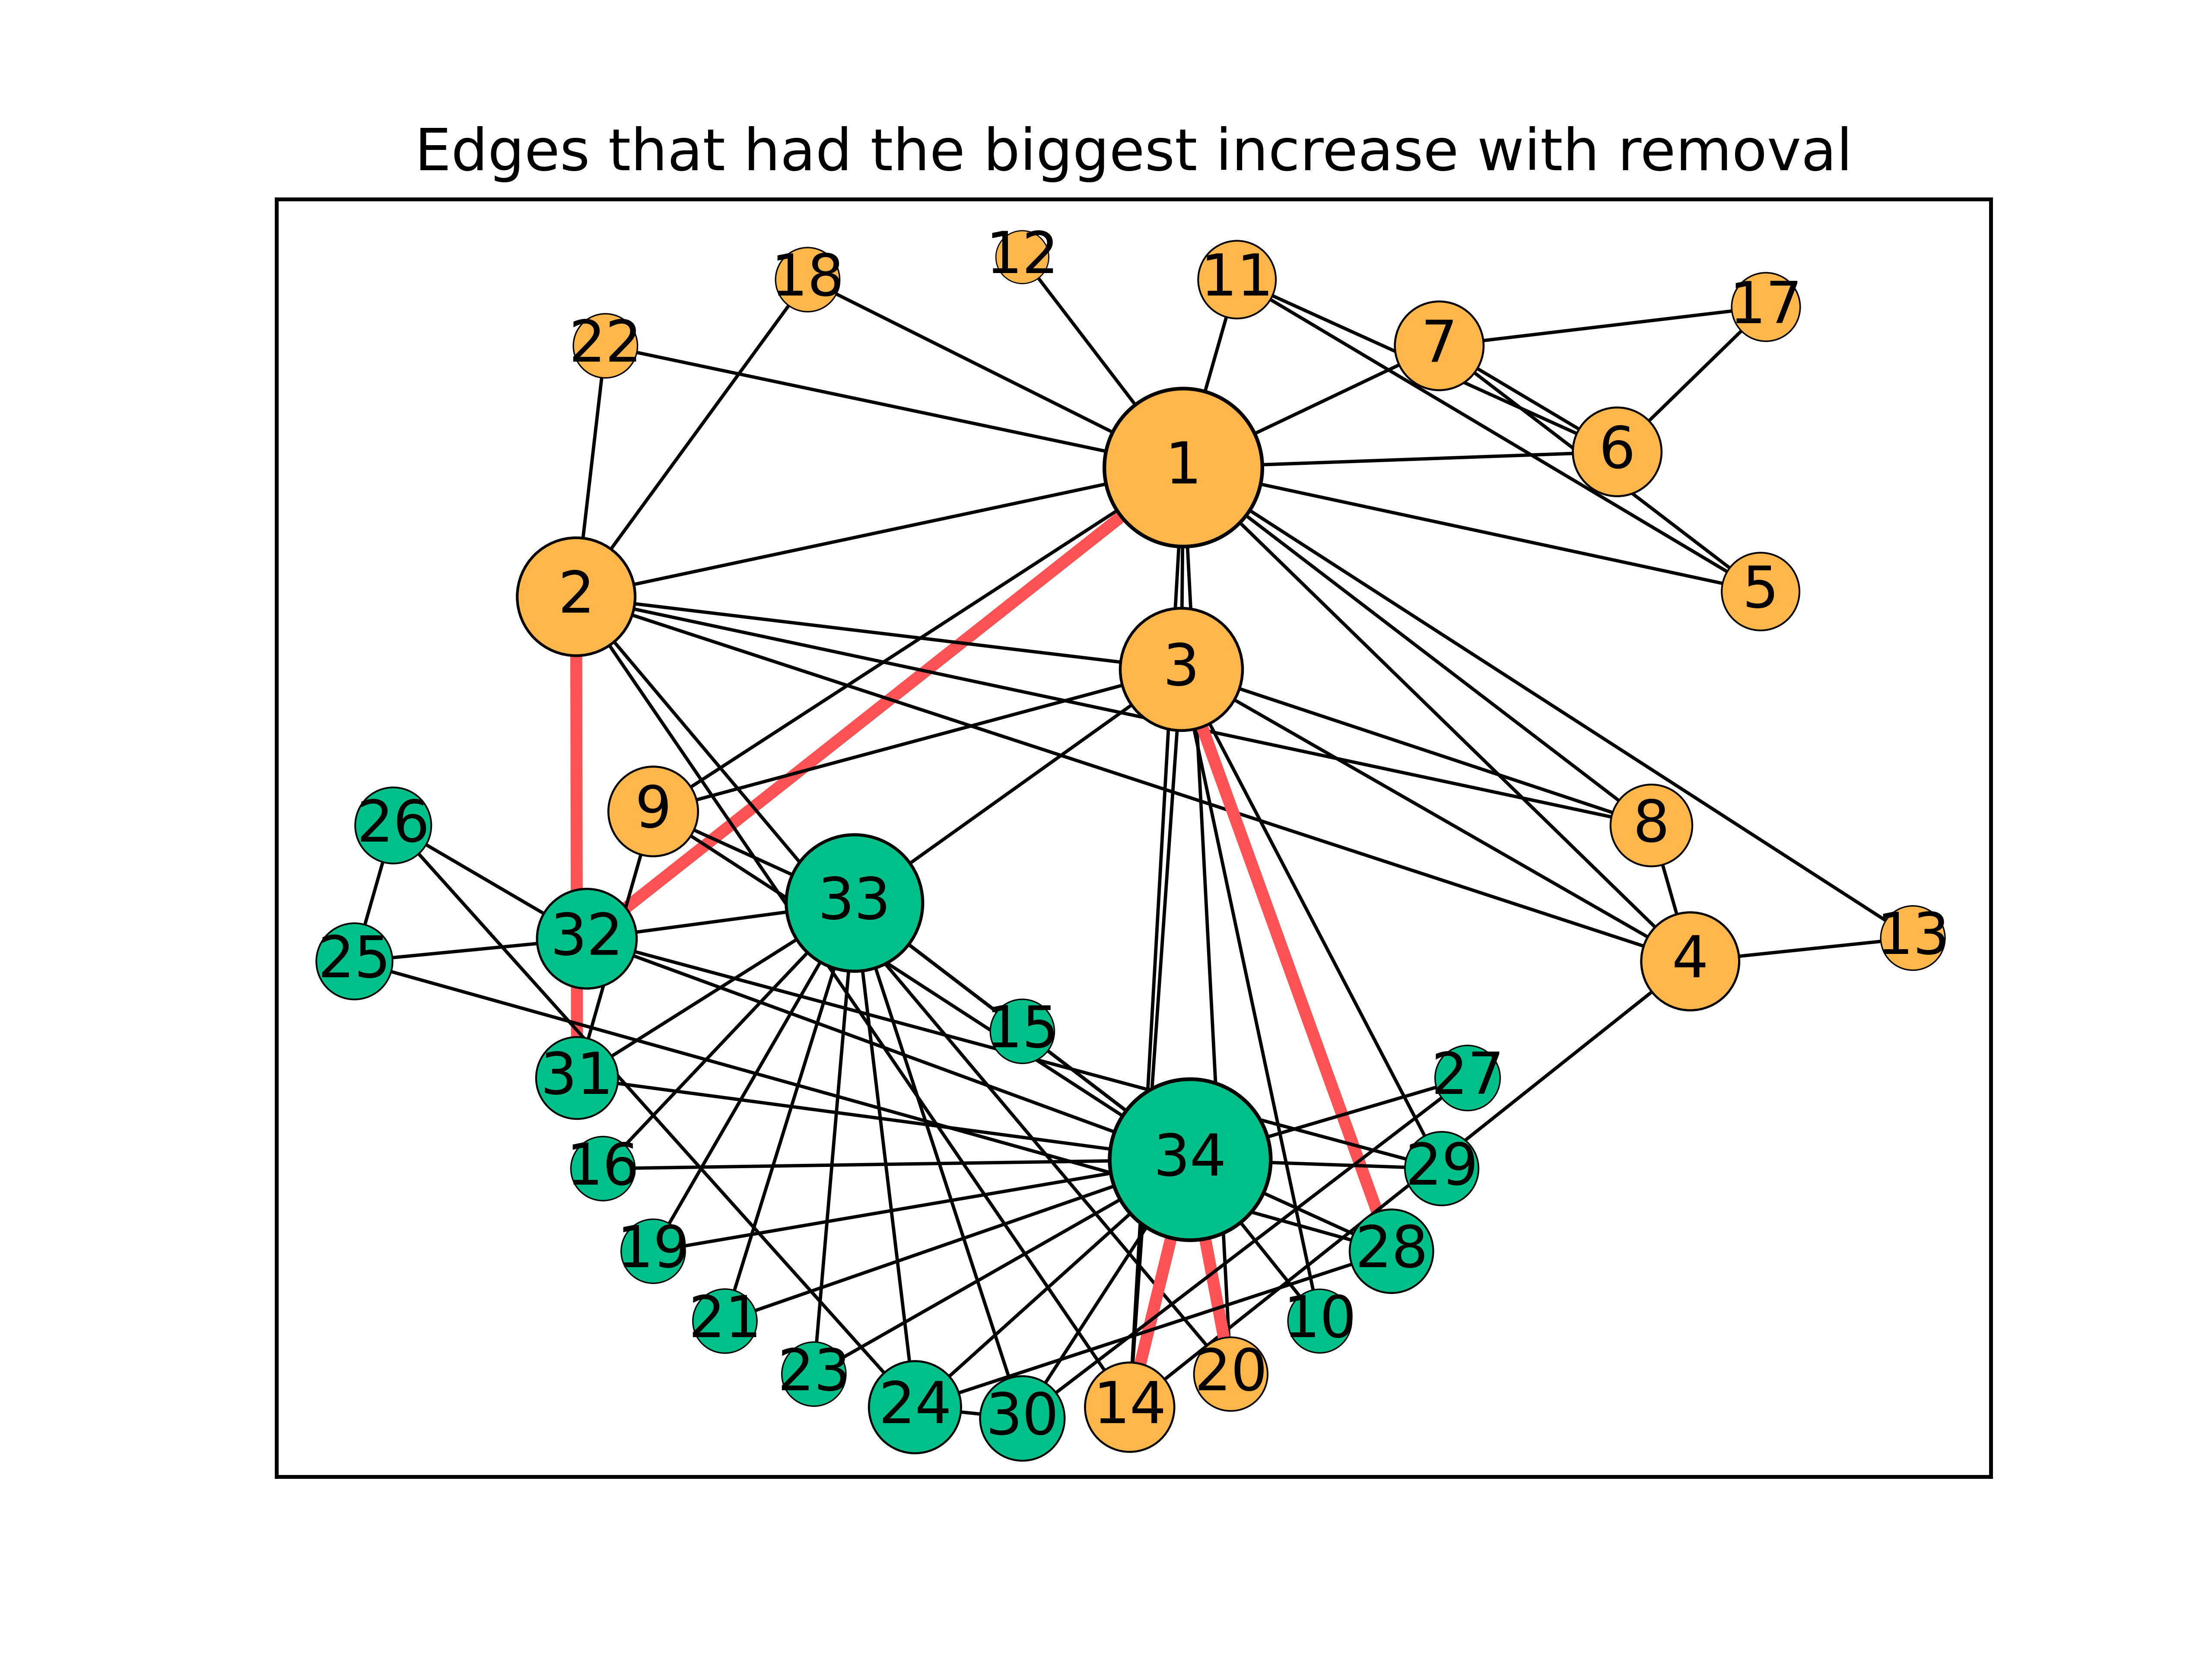
\includegraphics[width=0.65\textwidth]{Figures/karate_increase}
	\label{fig:karate_increase}
	\caption{Removing edges in Karate}
\end{figure}

\begin{figure}[H]
	\centering
	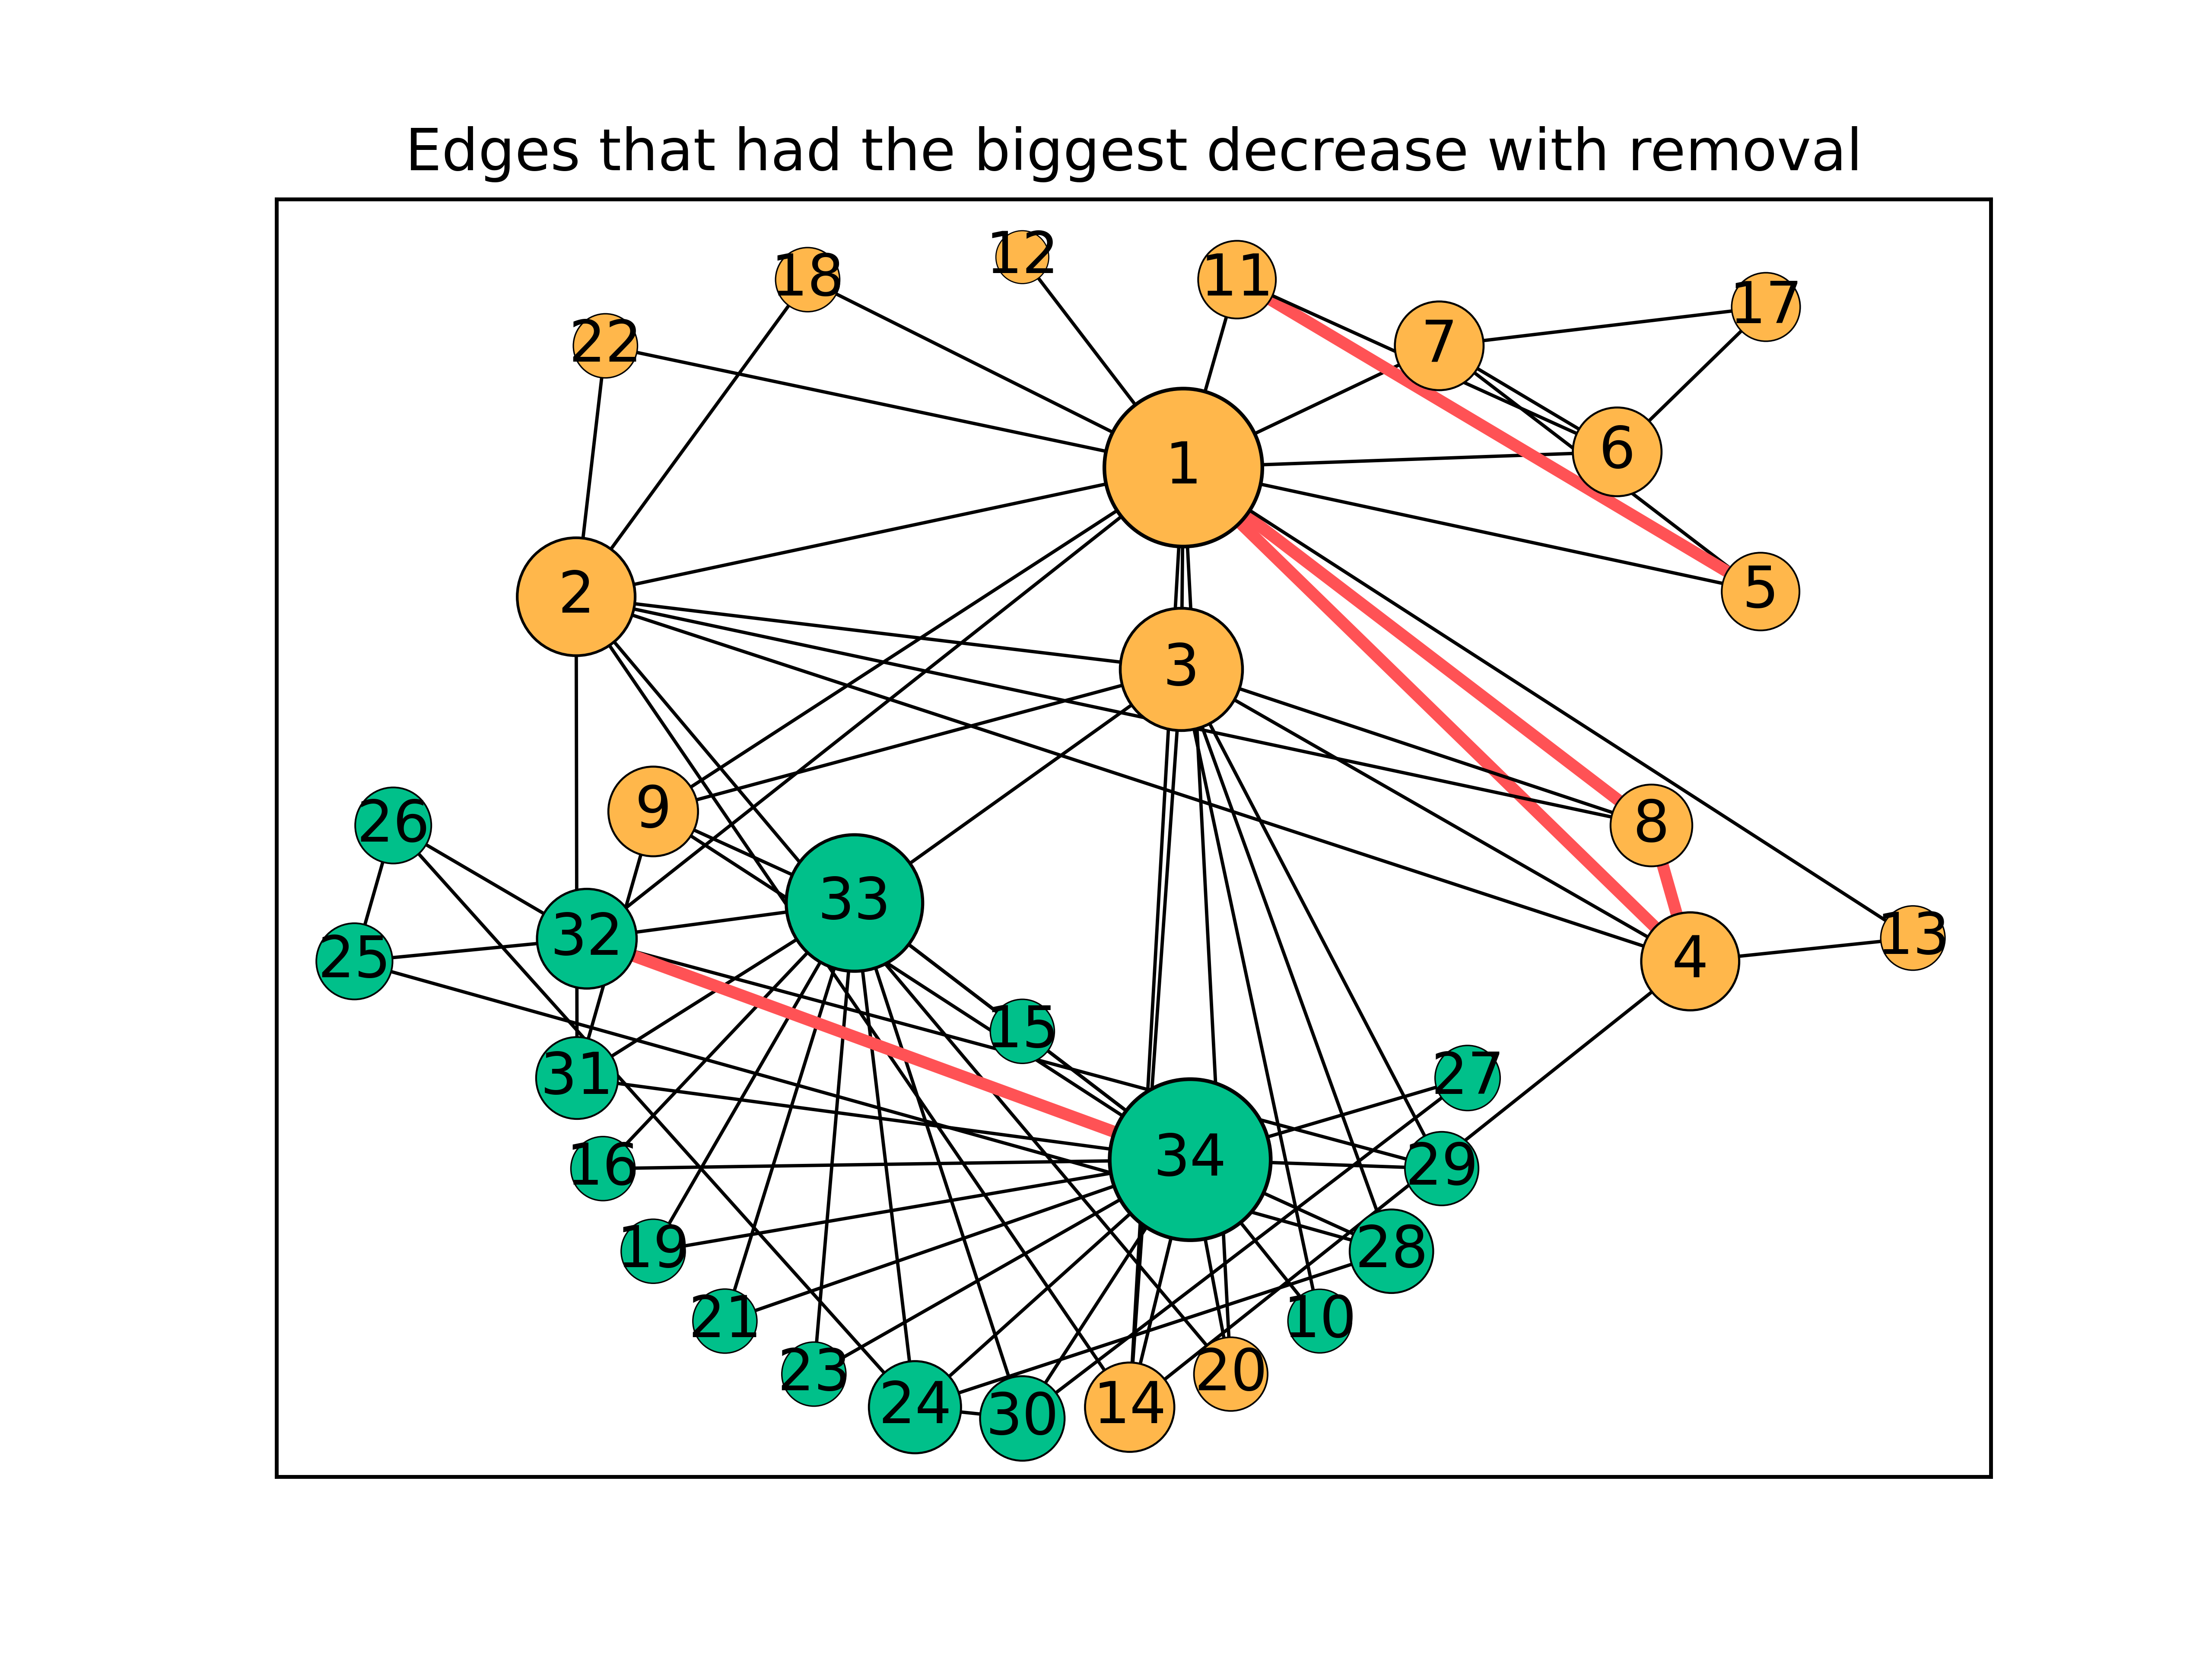
\includegraphics[width=0.65\textwidth]{Figures/karate_decrease}
	\label{fig:karate_decrease}
	\caption{Removing edges in Karate}
\end{figure}


\subsection{Edges removal in the Blogs dataset}

\begin{table}[H]
 \centering
 \caption{Edges with the biggest increase of polarization}
 \label{tab:edgesLargest}
 \begin{tabular}{| l || l | l | l | l |}
 \hline
  Edge & Betweenness Centrality & Polarization Increase & Sign & Addition\\
  \hline
  \hline
  (213, 793) & $0.00219$ & $0.00091$ & - &  0\\
  \hline
  (600, 1183) & $0.00439$ & $0.00074$ & - &  0\\
  \hline
  (523, 1375) & $0.00110$ & $0.00070$ & - &  0\\
  \hline
  (325, 1159) & $0.00110$ & $0.00069$ & - &  0\\
  \hline
  (632, 1000) & $0.00110$ & $0.00069$ & - &  0\\
  \hline
 \end{tabular}
 
 
 \caption{Edges with the biggest decrease of polarization }
 \label{tab:edgesLargest}
 \begin{tabular}{| l || l | l | l | l |}
 \hline
  Edge & Betweenness Centrality & Polarization Decrease & Sign & Addition\\
  \hline
  \hline
  (574, 1380) & $0.00014$ & $2.09620*10^{-6}$ & - &  0\\
  \hline
  (23, 1380) & $0.00021$ & $2.18102*10^{-6}$ & - &  0\\
  \hline
  (600, 1021) & $0.00024$ & $2.41460*10^{-6}$ & - &  0\\
  \hline
  (634, 1380) & $0.00010$ & $2.60119*10^{-6}$ & - &  0\\
  \hline
  (219, 1380) & $0.00014$ & $2.91467*10^{-6}$ & - &  0\\
  \hline
  \hline
 \end{tabular}
 
\end{table}

\subsection{Edges removal in the Books dataset}
\begin{table}[H]
 \centering
 \caption{Edges with the biggest increase of polarization }
 \label{tab:edgesLargest}
 \begin{tabular}{| l || l | l | l | l |}
 \hline
  Edge & Betweenness Centrality & Polarization Increase & Sign & Addition\\
  \hline
  \hline
  (0, 5) & $0.00056$ & $2.65885*10^5$ & - &  0\\
  \hline
  (7, 58) & $0.00713$ & $0.00012$ & - &  0\\
  \hline
  (5, 6) & $0.00222$ & $0.00012$ & - &  0\\
  \hline
  (6, 18) & $0.00858$ & $0.00014$ & +& -2\\
  \hline
  (0, 2) & $0.00031$ & $0.00349$ & - &  0\\
  \hline
 \end{tabular}
\end{table}

\begin{table}[H]
 \centering
 \caption{Edges with the biggest decrease of polarization}
 \label{tab:edgesLargest}
 \begin{tabular}{| l || l | l | l | l |}
 \hline
  Edge & Betweenness Centrality & Polarization Decrease & Sign & Addition\\
  \hline
  \hline
  (53, 76) & $0.06290$ & $0.01985$ & - &  0\\
  \hline
  (46, 102) & $0.04914$ & $0.01541$ & + &  -2\\
  \hline
  (19, 77) & $0.04367$ & $0.01458$ & + &  +2\\
  \hline
  (9, 51) & $0.02812$ & $0.01000$ & - &  0\\
  \hline
  (49, 72) & $0.06809$ & $0.00952$ & - &  0\\
  \hline
 \end{tabular} 
\end{table}

\subsection{Remarks about the edge removals}

We can clearly see that there is an association between the edge betweenness centrality and the decrease in polarization. Edges that contribute to a bigger decrease have larger betweenness centrality. 
\\
\\
A second thing that we see in all three datasets is that the biggest increase is coming from the removal of edges that connect opposing opinions.
\\
\\
In addition, during the experiments on the karate dataset, the removal of edge $(6, 7)$ had no effect on the polarization index. This leads to the following lemma.

\begin{lemma}
The polarization index can stay the same after an edge removal.
\end{lemma}



% Εισαγωγή της βιβλιογραφίας
\addstarredchapterc{\bibname} % minitoc
\bibliographystyle{IEEEtran}
\bibliography{/Users/leonidas/Desktop/Spring2020/thesis/LaTeXthesis/Template/Content/Bibliography}

% Προαιρετικά, μπορείτε να εισάγετε παραρτήματα
%\appendix 
%\chapter{Τίτλος πρώτου παραρτήματος}
\label{app:FirstAppendix}

Εδώ είναι ο χώρος του πρώτου Παραρτήματος.

\begin{table}[h]
	\centering
	\caption{Πίνακας Παραρτήματος.}
	\label{tab:AppendixTable}
	\begin{tabular}{l l l l l}
		\hline
		~ & ~ & Sample Mean & ~ & 95\% Confidence Interval \\
		\hline
		1 process & ~ & $3.640966$  & ~ & $0.100136$ \\
		4 processes & ~ & $1.053655$  & ~ & $0.037212$ \\
		8 processes & ~ & $0.610223$  & ~ & $0.023470$ \\
		16 processes & ~ & $0.357321$  & ~ & $0.014783$ \\
		32 processes & ~ & $0.227180$  & ~ & $0.016923$ \\
		\hline
	\end{tabular}
\end{table}
%\chapter{Τίτλος δεύτερου παραρτήματος}
\label{app:SecondAppendix}

\section{Τίτλος πρώτης ενότητας}
\label{sec:FirstSection}
Εδώ είναι ο χώρος της πρώτης ενότητας του δεύτερου Παραρτήματος.

\section{Τίτλος δεύτερης ενότητας}
\label{sec:SecondSection}
Εδώ είναι ο χώρος της δεύτερης ενότητας του δεύτερου Παραρτήματος.
%\chapter{Τίτλος τρίτου παραρτήματος}
\label{app:ThirdAppendix}

Εδώ είναι ο χώρος του τρίτου Παραρτήματος.

\begin{figure}[h]
	\centering
	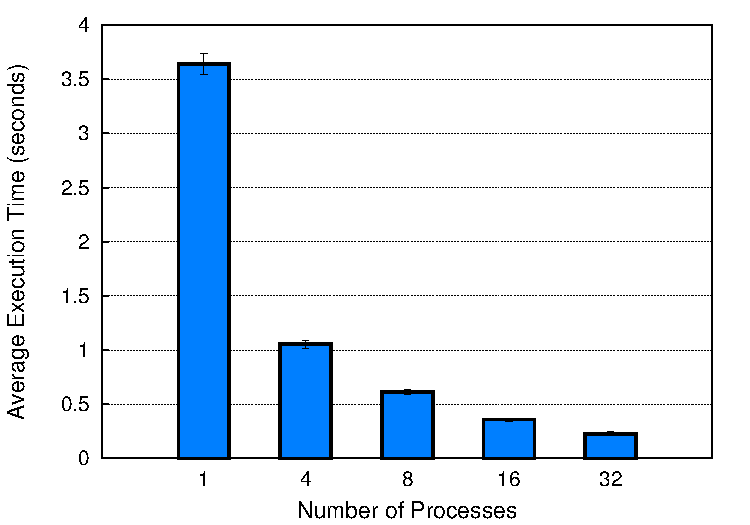
\includegraphics[width=0.65\textwidth]{Figures/MatrixMultiplication.pdf}
	\caption{Εικόνα Παραρτήματος.}
	\label{fig:AppendixFigure}
\end{figure}


% Εκτύπωση του ευρετηρίου (προαιρετικό)
%\printindex


% Σελίδες χωρίς αρίθμηση
\pagenumbering{gobble}

%\pdfbookmark[0]{\csedimosieuseis}{dimosieuseis} % hyperref
\chapter*{\csedimosieuseis}

Προαιρετικά, βάζουμε μία λίστα με τις δημοσιεύσεις του συγγραφέα. % Προαιρετικό

% Σύντομο Βιογραφικό
%\pdfbookmark[0]{\cseviografiko}{viografiko} % hyperref
\chapter*{\cseviografiko}

Ένα σύντομο βιογραφικό είναι απαραίτητο.

\end{document}
